
% Document class and paper format:
\documentclass[a4paper,12pt]{article}
\usepackage[a4paper, left=2cm, right=2cm, top=2cm, bottom=2cm]{geometry}
\pagestyle{empty}


% Language & Encoding
\usepackage[catalan]{babel}
\usepackage[utf8]{inputenc}
\usepackage[T1]{fontenc}
\def\xgem{%
    \ifmmode
        \csname normal@char\string"\endcsname l%
    \else
        \leftllkern=0pt\rightllkern=0pt\raiselldim=0pt
        \setbox0\hbox{l}\setbox1\hbox{l\/}\setbox2\hbox{.}%
        \advance\raiselldim by \the\fontdimen5\the\font
        \advance\raiselldim by -\ht2
        \leftllkern=-.25\wd0%
        \advance\leftllkern by \wd1
        \advance\leftllkern by -\wd0
        \rightllkern=-.25\wd0%
        \advance\rightllkern by -\wd1
        \advance\rightllkern by \wd0
        \allowhyphens\discretionary{-}{}%
        {\kern\leftllkern\raise\raiselldim\hbox{.}%
        \kern\rightllkern}\allowhyphens
    \fi
}
\def\Xgem{%
    \ifmmode
        \csname normal@char\string"\endcsname L%
    \else
        \leftllkern=0pt\rightllkern=0pt\raiselldim=0pt
        \setbox0\hbox{L}\setbox1\hbox{L\/}\setbox2\hbox{.}%
        \advance\raiselldim by .5\ht0
        \advance\raiselldim by -.5\ht2
        \leftllkern=-.125\wd0%
        \advance\leftllkern by \wd1
        \advance\leftllkern by -\wd0
        \rightllkern=-\wd0%
        \divide\rightllkern by 6
        \advance\rightllkern by -\wd1
        \advance\rightllkern by \wd0
        \allowhyphens\discretionary{-}{}%
        {\kern\leftllkern\raise\raiselldim\hbox{.}%
        \kern\rightllkern}\allowhyphens
    \fi
}
\DeclareTextCommand{\textperiodcentered}{T1}[1]{%
    \ifnum\spacefactor=998
        \Xgem
    \else
        \xgem
    \fi#1}


% Paragraph formating
\usepackage{parskip}
\setlength{\parindent}{0pt}
\frenchspacing


% Sans serif font:
\usepackage[protrusion=true,expansion=true,final]{microtype}
\usepackage{moresize}
\usepackage{paratype}
\renewcommand{\familydefault}{\sfdefault}
%\usepackage{sansmath}
%\sansmath


% Include Diagrams:
\usepackage{xcolor}
\usepackage{amssymb} % for \bigstar
\usepackage{rotating}
\usepackage{tikz}
\usetikzlibrary{calc}
\usepackage{pdfpages}


% Adjustements for MMACA's Logo:
\setlength{\fboxsep}{5pt}
\setlength{\fboxrule}{0.75pt}


% \today's formatting:
\usepackage[yyyymmdd]{datetime}
%\renewcommand{\dateseparator}{}


% Hyperlink's format:
\usepackage{hyperref}
\hypersetup {
    hidelinks,
    pagebackref  = true,
    pdfauthor    = {Carlos Luna Mota},
    pdfsubject   = {Spira Mirabilis},
    pdftitle     = {Spira Mirabilis},
    pdfkeywords  = {spira, mirabilis, logarithmic, spirals, proportions, MMACA},
    pdfcreator   = {LaTeX},
    pdfproducer  = {pdflatex}
}
\urlstyle{same}

%%% DOCUMENT %%%%%%%%%%%%%%%%%%%%%%%%%%%%%%%%%%%%%%%%%%%%%%%%%%%%%%%%%%%%%%%%%%%

\begin{document}

    %%% FRONTPAGE %%%%%%%%%%%%%%%%%%%%%%%%%%%%%%%%%%%%%%%%%%%%%%%%%%%%%%%%%%%%%%

    \begin{center}

        \phantom{.}
        \bigskip

        {\HUGE \bf Spira Mirabilis}

        \bigskip  

        \centering{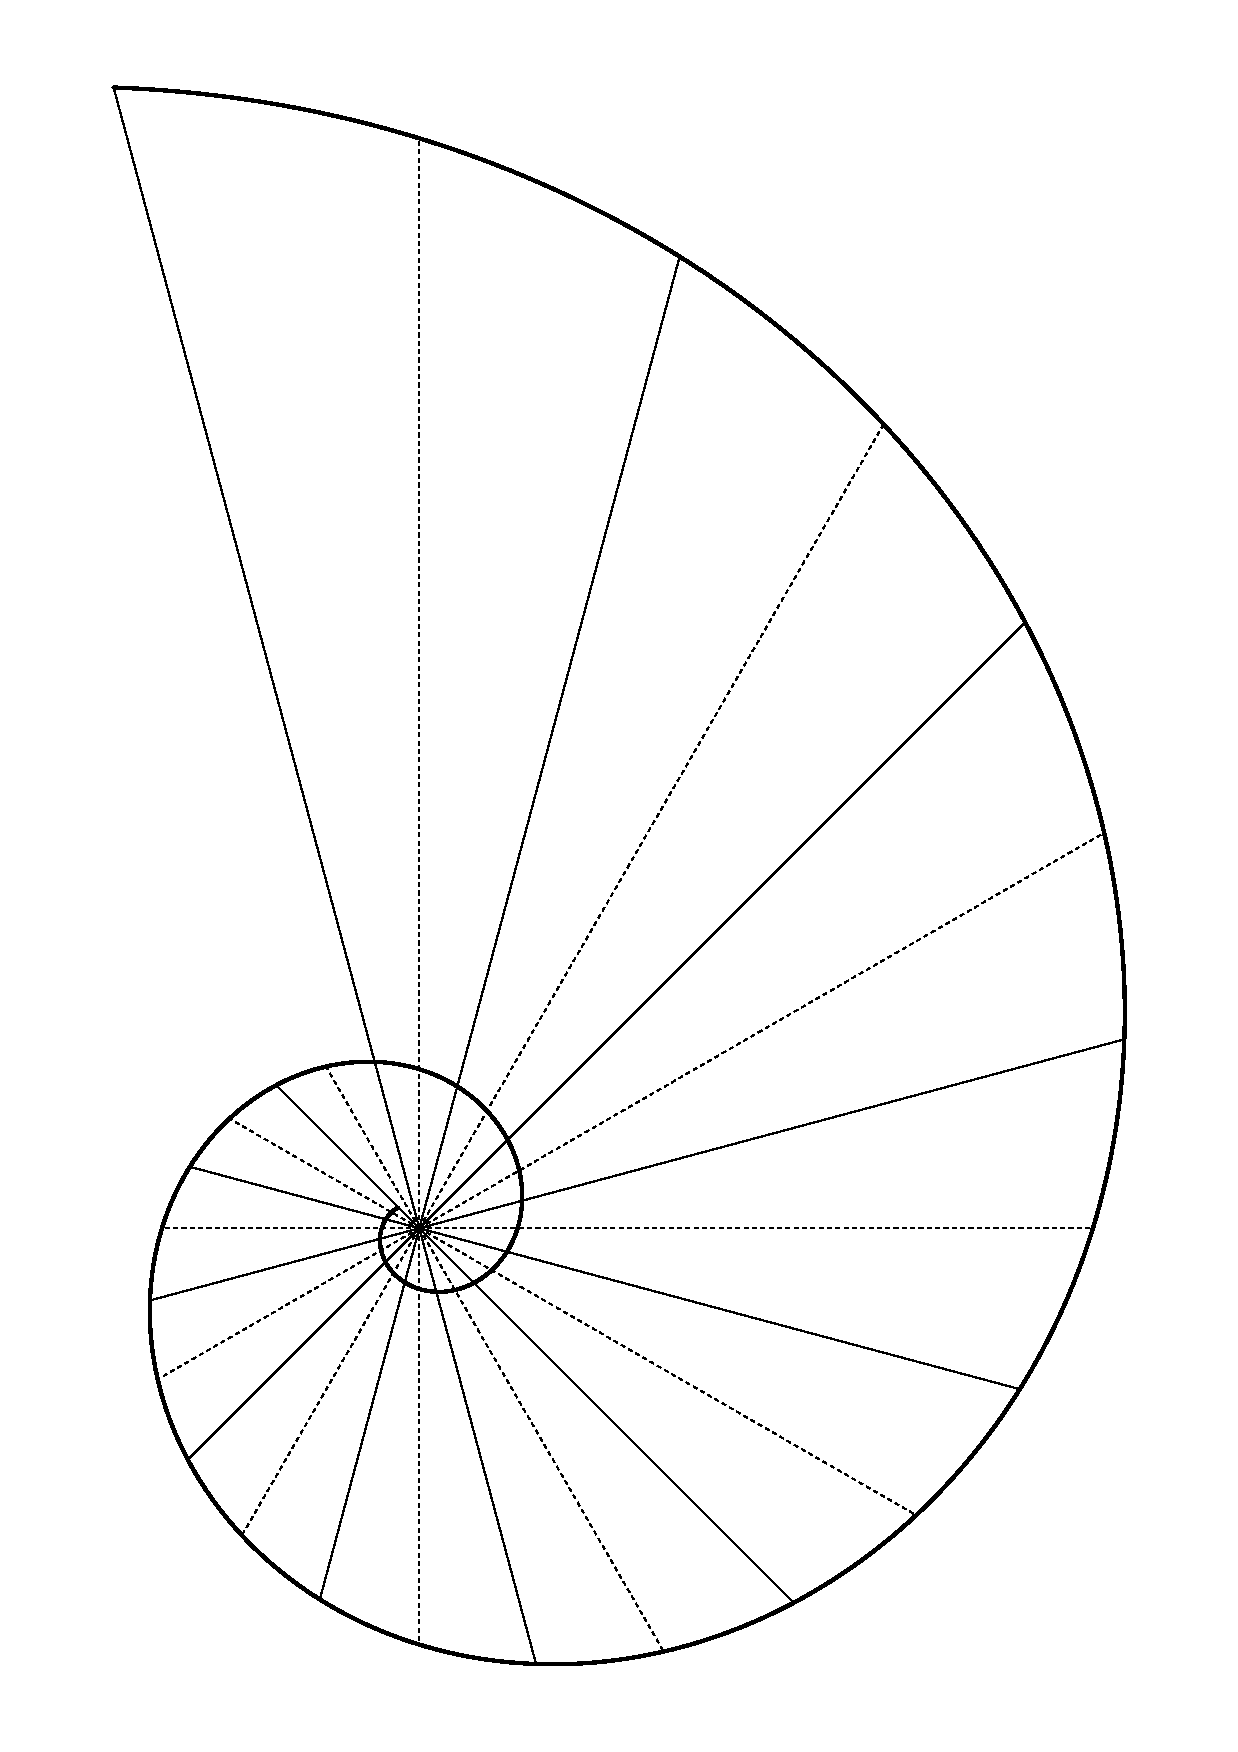
\includegraphics[scale=0.7071]{./pictures/Example_00}}
        
        \bigskip 

        \href{https://mmaca.cat/}{\Huge \fcolorbox{white}{black}{\color{white}\textbf{mmaca}}}
    \end{center}

    \newpage

    %%% CREDITS %%%%%%%%%%%%%%%%%%%%%%%%%%%%%%%%%%%%%%%%%%%%%%%%%%%%%%%%%%%%%%%%

    \phantom{.}
    \vspace{40em}

    \textbf{Spira Mirabilis} is a teaching aid developed\\at the \textbf{Catalan Museum of Mathematics}.\\\href{https://mmaca.cat/}{https://mmaca.cat/}\\[0.25ex]

    Feel free to print this document for teaching purposes.\\[1ex]

    \begin{tabular}{rl}
        \hspace{-0.6em}\textbf{License:} & \hspace{-1em} \href{https://creativecommons.org/licenses/by-nc-sa/4.0/}{CC BY-NC-SA 4.0}\\
        \hspace{-0.6em}\textbf{Author:}  & \hspace{-1em} \href{https://github.com/CarlosLunaMota}{Carlos Luna Mota}\\
        \hspace{-0.6em}\textbf{Version:} & \hspace{-1em} \today\\
    \end{tabular}

    \newpage

    %%% INTRODUCTION %%%%%%%%%%%%%%%%%%%%%%%%%%%%%%%%%%%%%%%%%%%%%%%%%%%%%%%%%%%

    \phantom{.}
    \vspace{31em}

    {\huge \bf Spira Mirabilis}

    {\large \bigskip \bigskip

    Logarithmic spirals are a family of self-similar spiral curves that are characterized by their radius growing in geometric progression as they rotate.

    Albrecht Dürer described the logarithmic spirals in 1525, but it was Jacob Bernoulli who called them \textbf{Spira Mirabilis}, \emph{«marvelous spirals»}, in 1692, because he was fascinated by their unique mathematical properties.

    In this document, we use the notation \emph{«$\lambda \, / \, \alpha$ spiral»} to refer to the particular logarithmic spiral whose radius gets multiplied by $\lambda$ after rotating an angle $\alpha$.

    For example, the radius of the \emph{«$2 \, / \, 90^{\circ}$ spiral»} gets multiplied by $2$ every $90^{\circ}$, which means that it will be 16 times longer after a full turn.

    Below you can find some usage examples for these curves and a curated set of printable templates that are free to use for educational purposes.
    }

    \newpage

    %%% EXAMPLES %%%%%%%%%%%%%%%%%%%%%%%%%%%%%%%%%%%%%%%%%%%%%%%%%%%%%%%%%%%%%%%

    \phantom{.}
    \vspace{26em}

    {\huge \bf Spira Mirabilis examples}

    \bigskip

    {\large Read the red dots as the input and the blue dot as the output of each exercise}

    \newpage

    %%%%%%%%%%%%%%%%%%%%%%%%%%%%%%%%%%%%%%%%%%%%%%%%%%%%%%%%%%%%%%%%%%%%%%%%%%%%

    \begin{center}
    
        \large

        Divide a segment into thirds using the $3 \, / \, 360^{\circ}$ spiral

        \bigskip \bigskip \bigskip
    
        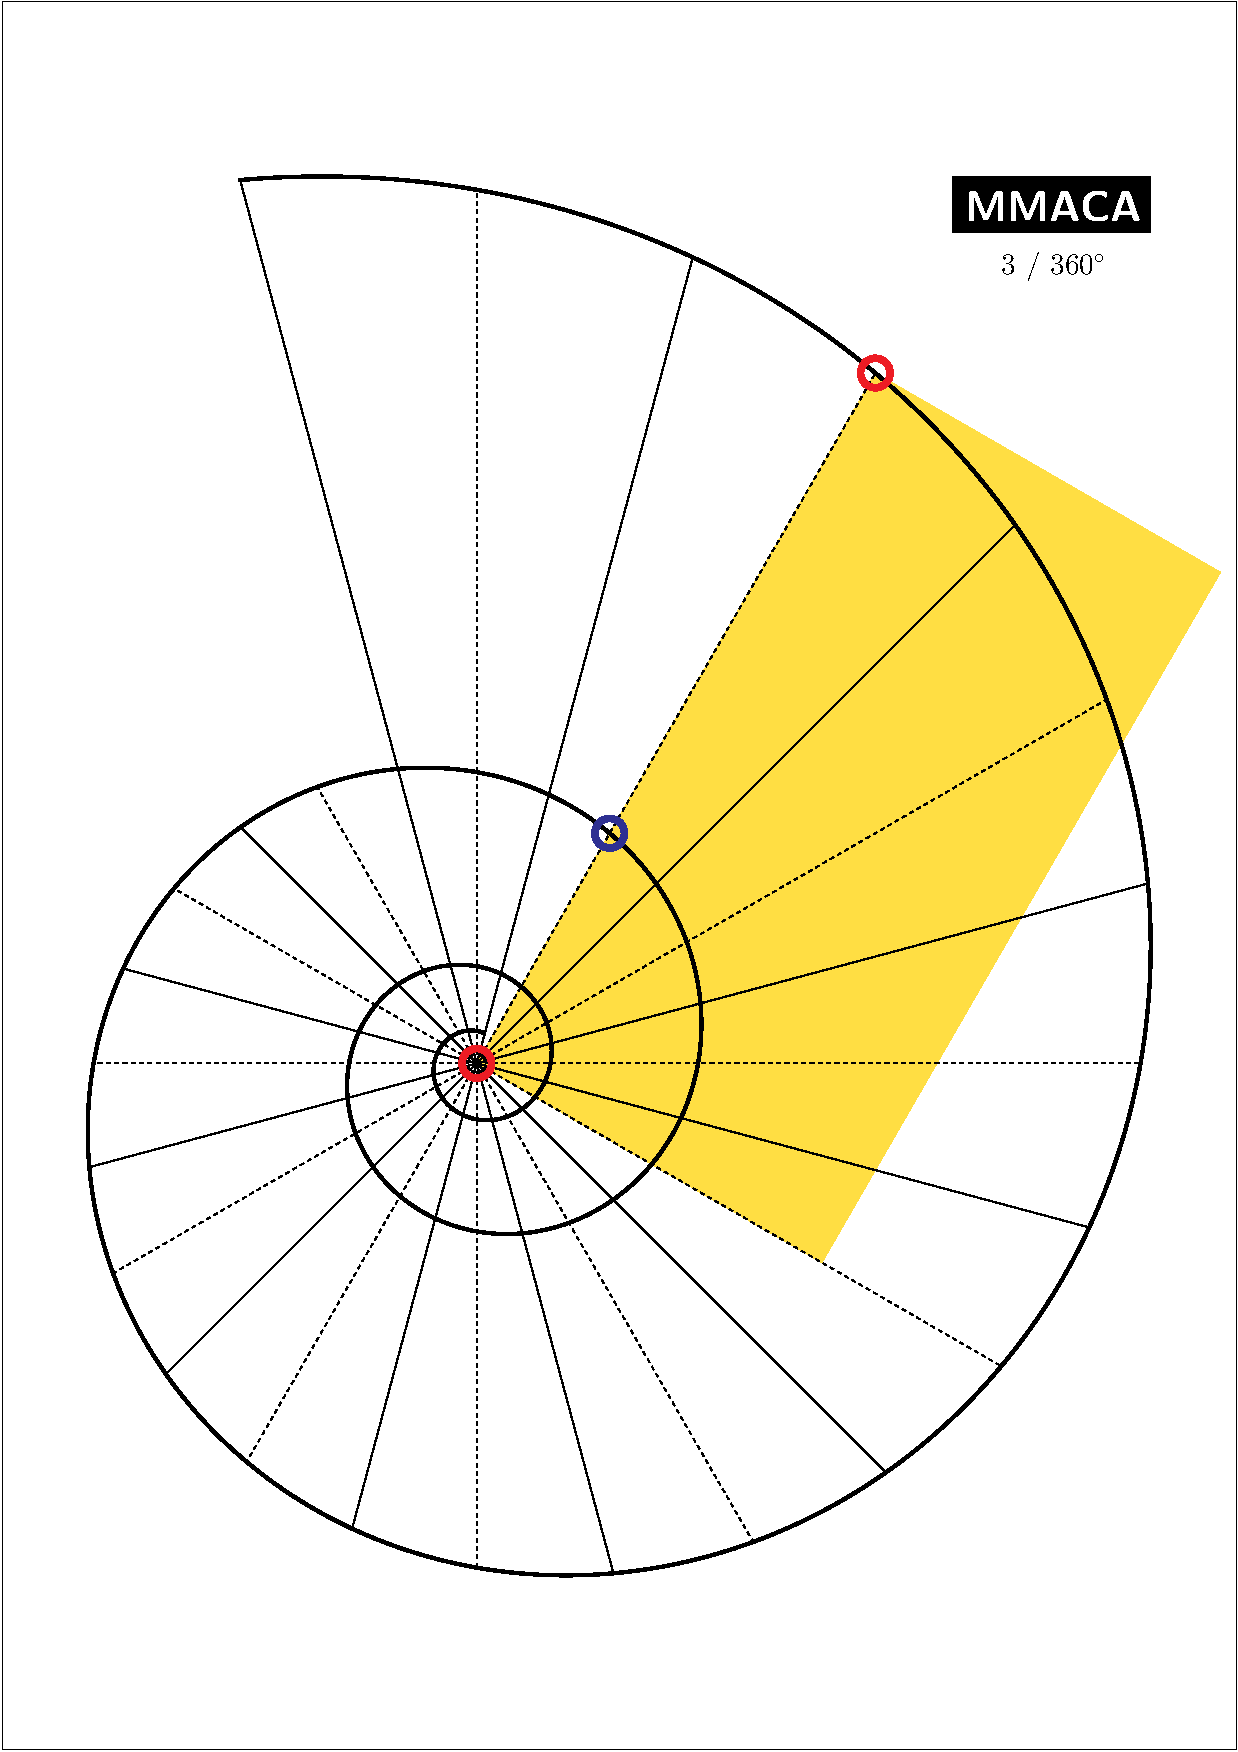
\includegraphics[scale=0.7071]{./pictures/Example_03}

    \end{center}

    \newpage

    %%%%%%%%%%%%%%%%%%%%%%%%%%%%%%%%%%%%%%%%%%%%%%%%%%%%%%%%%%%%%%%%%%%%%%%%%%%%

    \begin{center}
    
        \large

        Divide a segment into thirds using the $4 \, / \, 360^{\circ}$ spiral

        \bigskip \bigskip \bigskip
    
        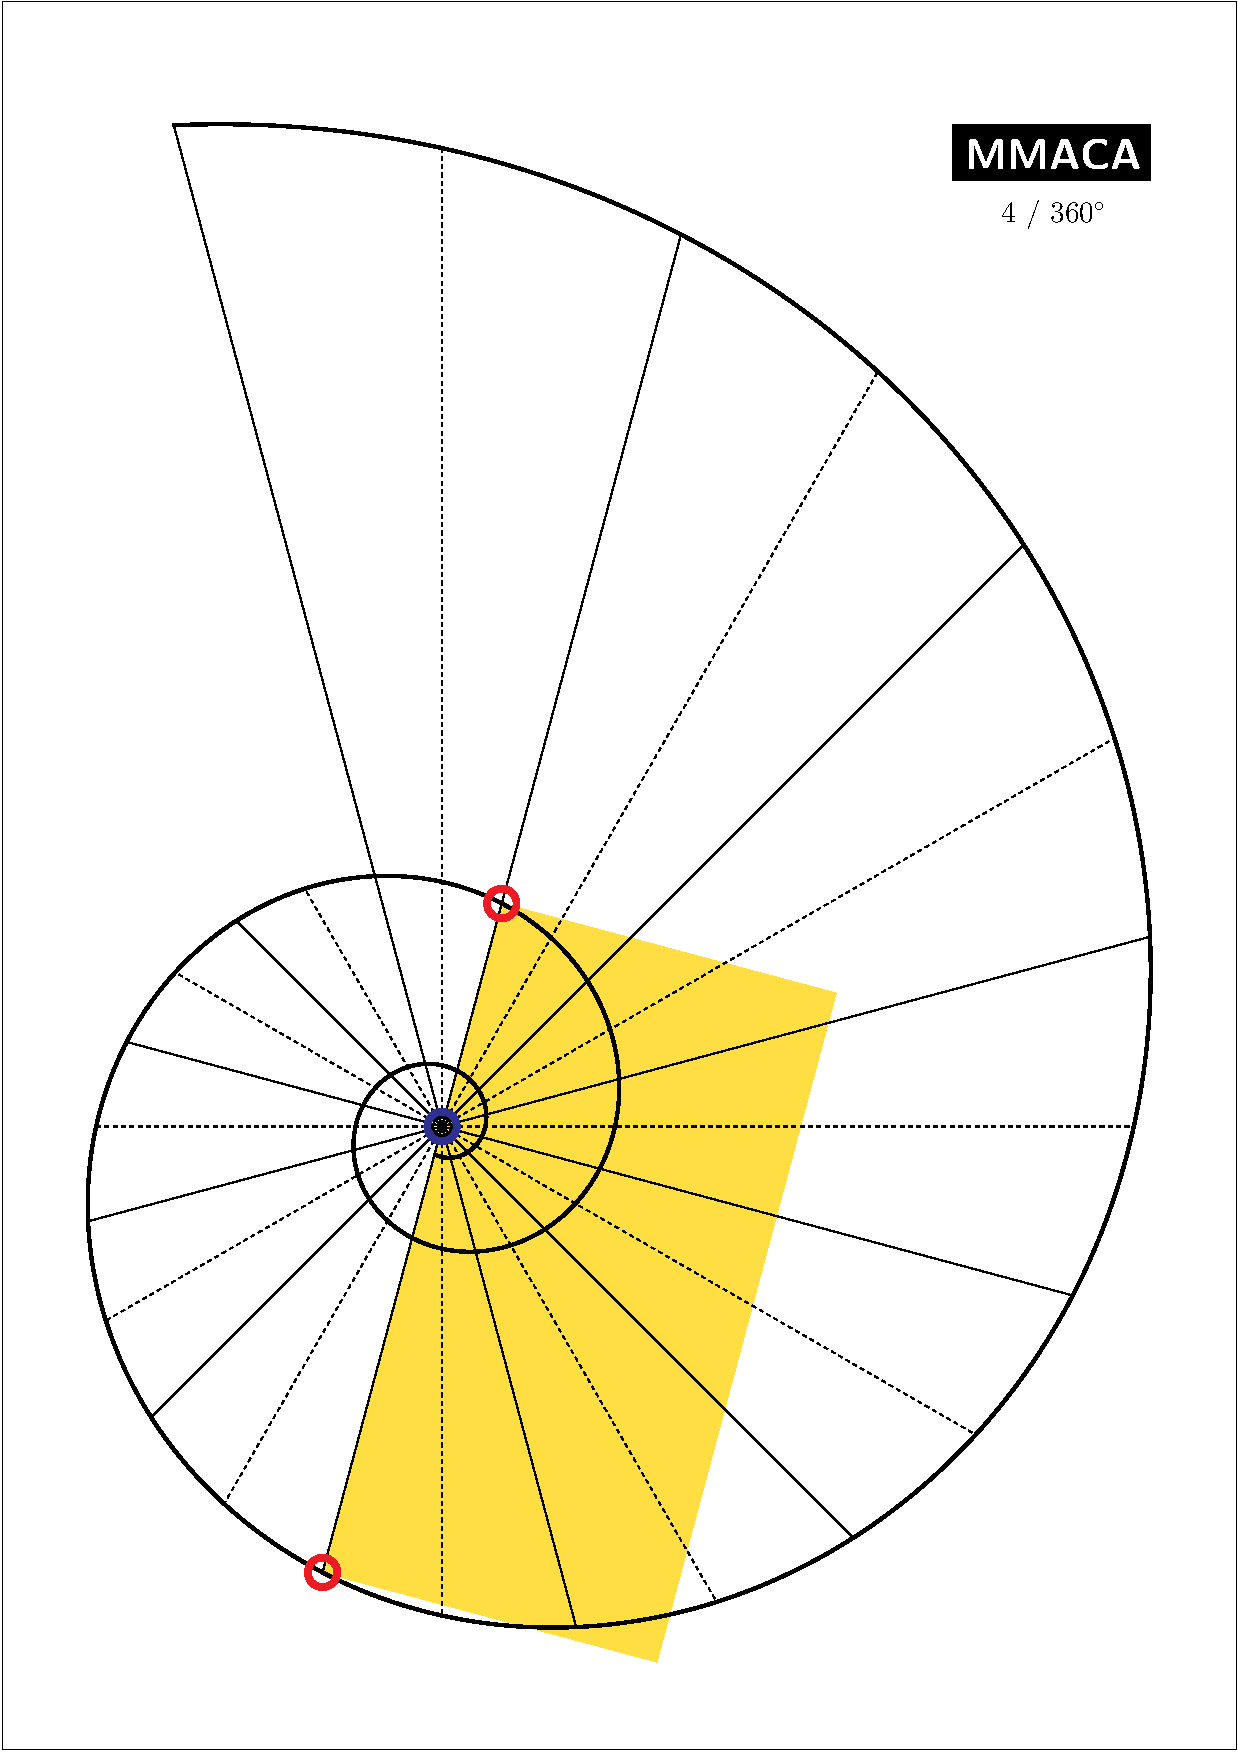
\includegraphics[scale=0.7071]{./pictures/Example_04}

    \end{center}

    \newpage

    %%%%%%%%%%%%%%%%%%%%%%%%%%%%%%%%%%%%%%%%%%%%%%%%%%%%%%%%%%%%%%%%%%%%%%%%%%%%

    \begin{center}
    
        \large

        Divide a segment by 8 using the $2 \, / \, 360^{\circ}$ spiral

        \bigskip \bigskip \bigskip
    
        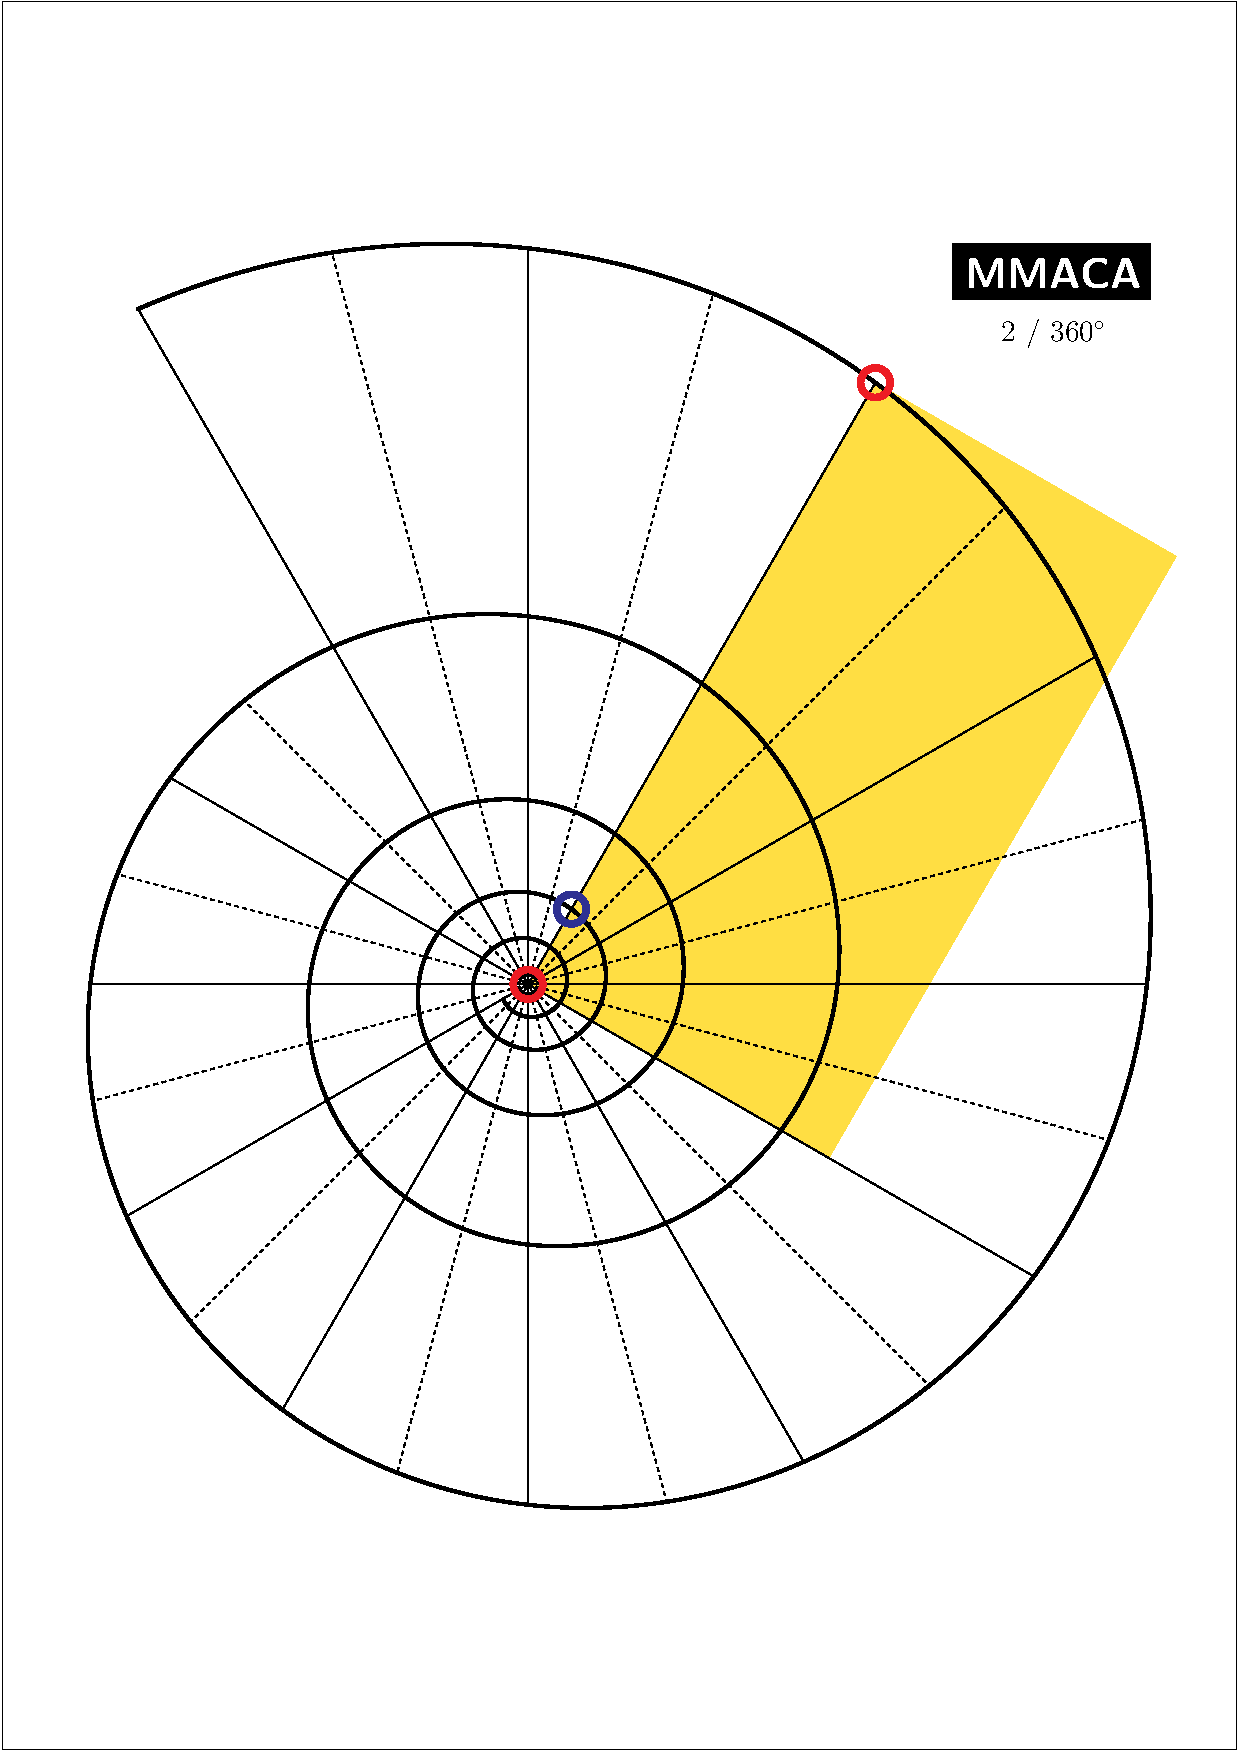
\includegraphics[scale=0.7071]{./pictures/Example_12}

    \end{center}

    \newpage

    %%%%%%%%%%%%%%%%%%%%%%%%%%%%%%%%%%%%%%%%%%%%%%%%%%%%%%%%%%%%%%%%%%%%%%%%%%%%

    \begin{center}
    
        \large

        Divide a segment by 9 using the $3 \, / \, 360^{\circ}$ spiral

        \bigskip \bigskip \bigskip
    
        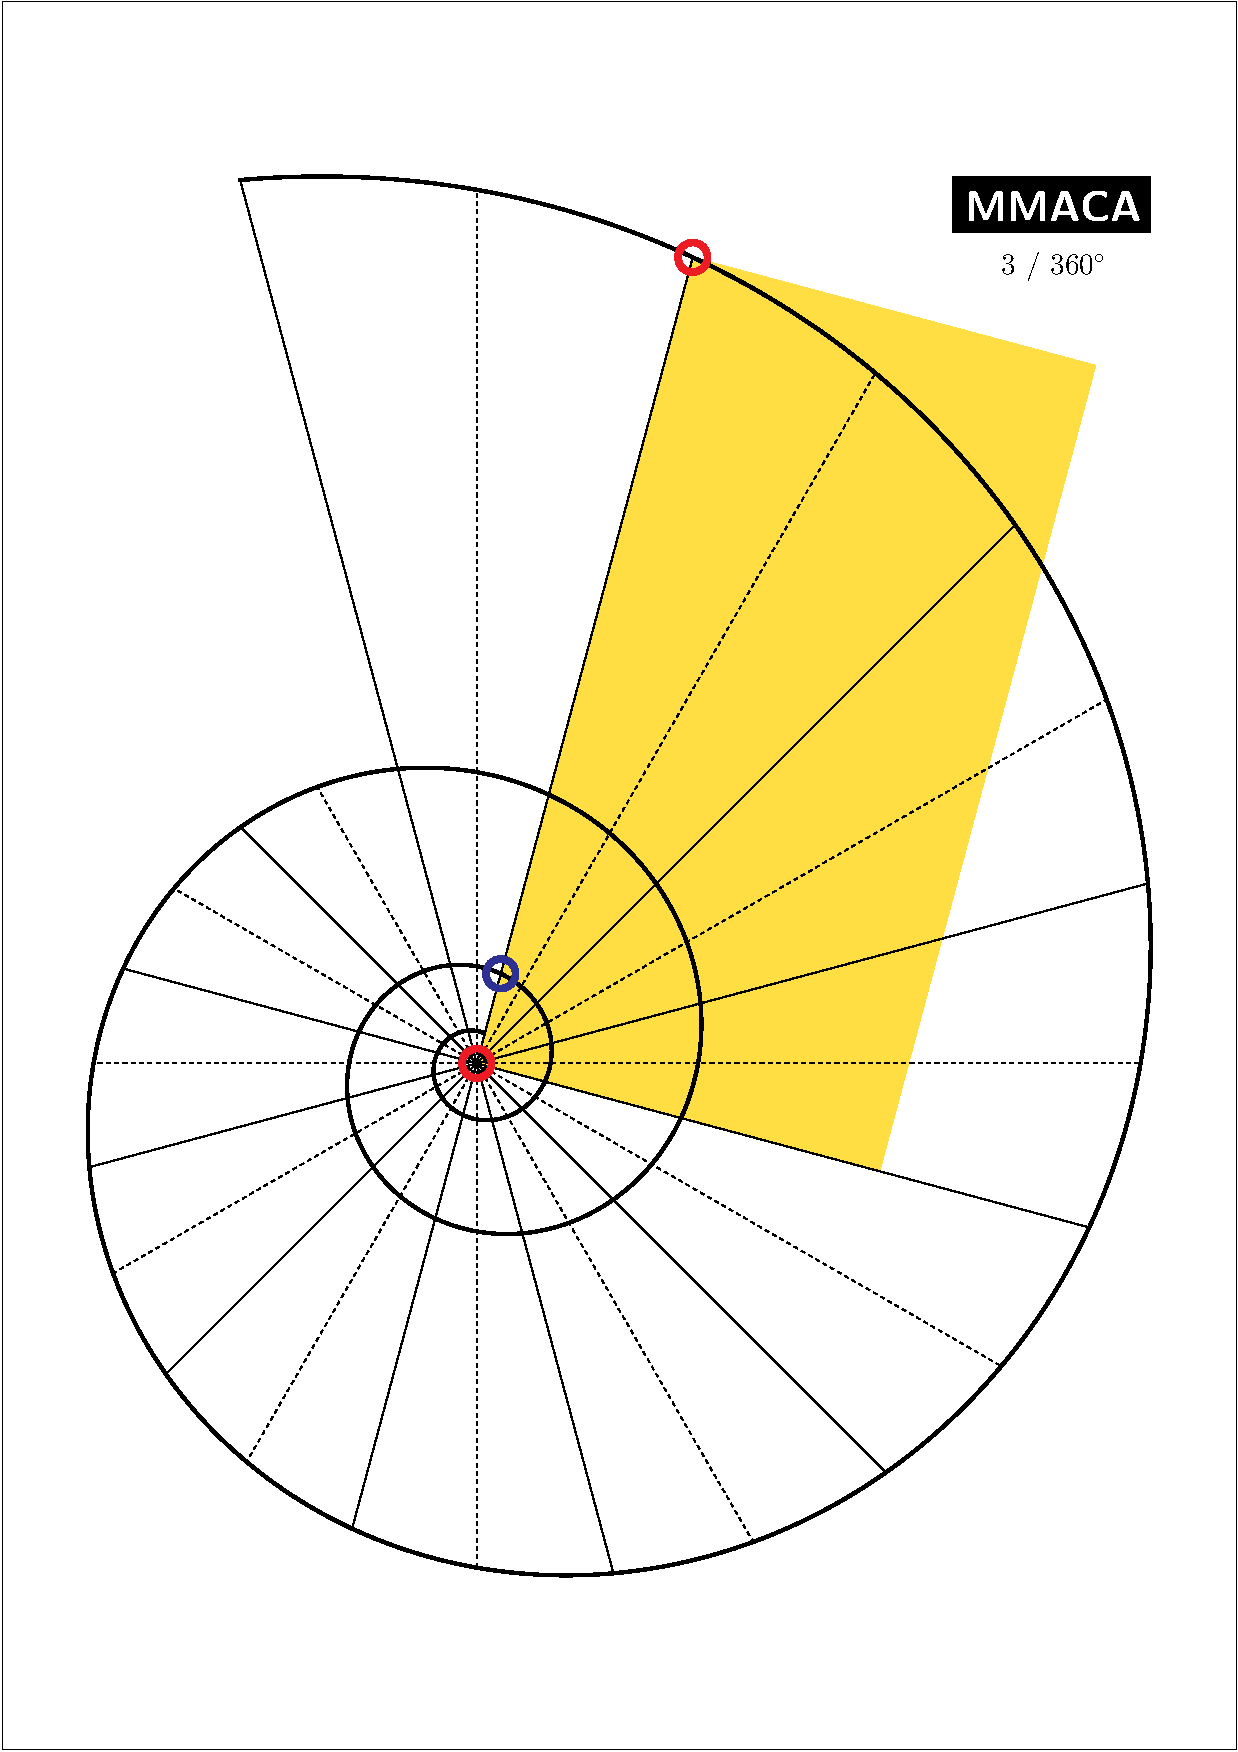
\includegraphics[scale=0.7071]{./pictures/Example_13}

    \end{center}

    \newpage

    %%%%%%%%%%%%%%%%%%%%%%%%%%%%%%%%%%%%%%%%%%%%%%%%%%%%%%%%%%%%%%%%%%%%%%%%%%%%

    \begin{center}
    
        \large

        Deduce the ratio of the sides of an A7 sheet of paper using the $\sqrt{2} \, / \, 90^{\circ}$ spiral

        \bigskip \bigskip \bigskip
    
        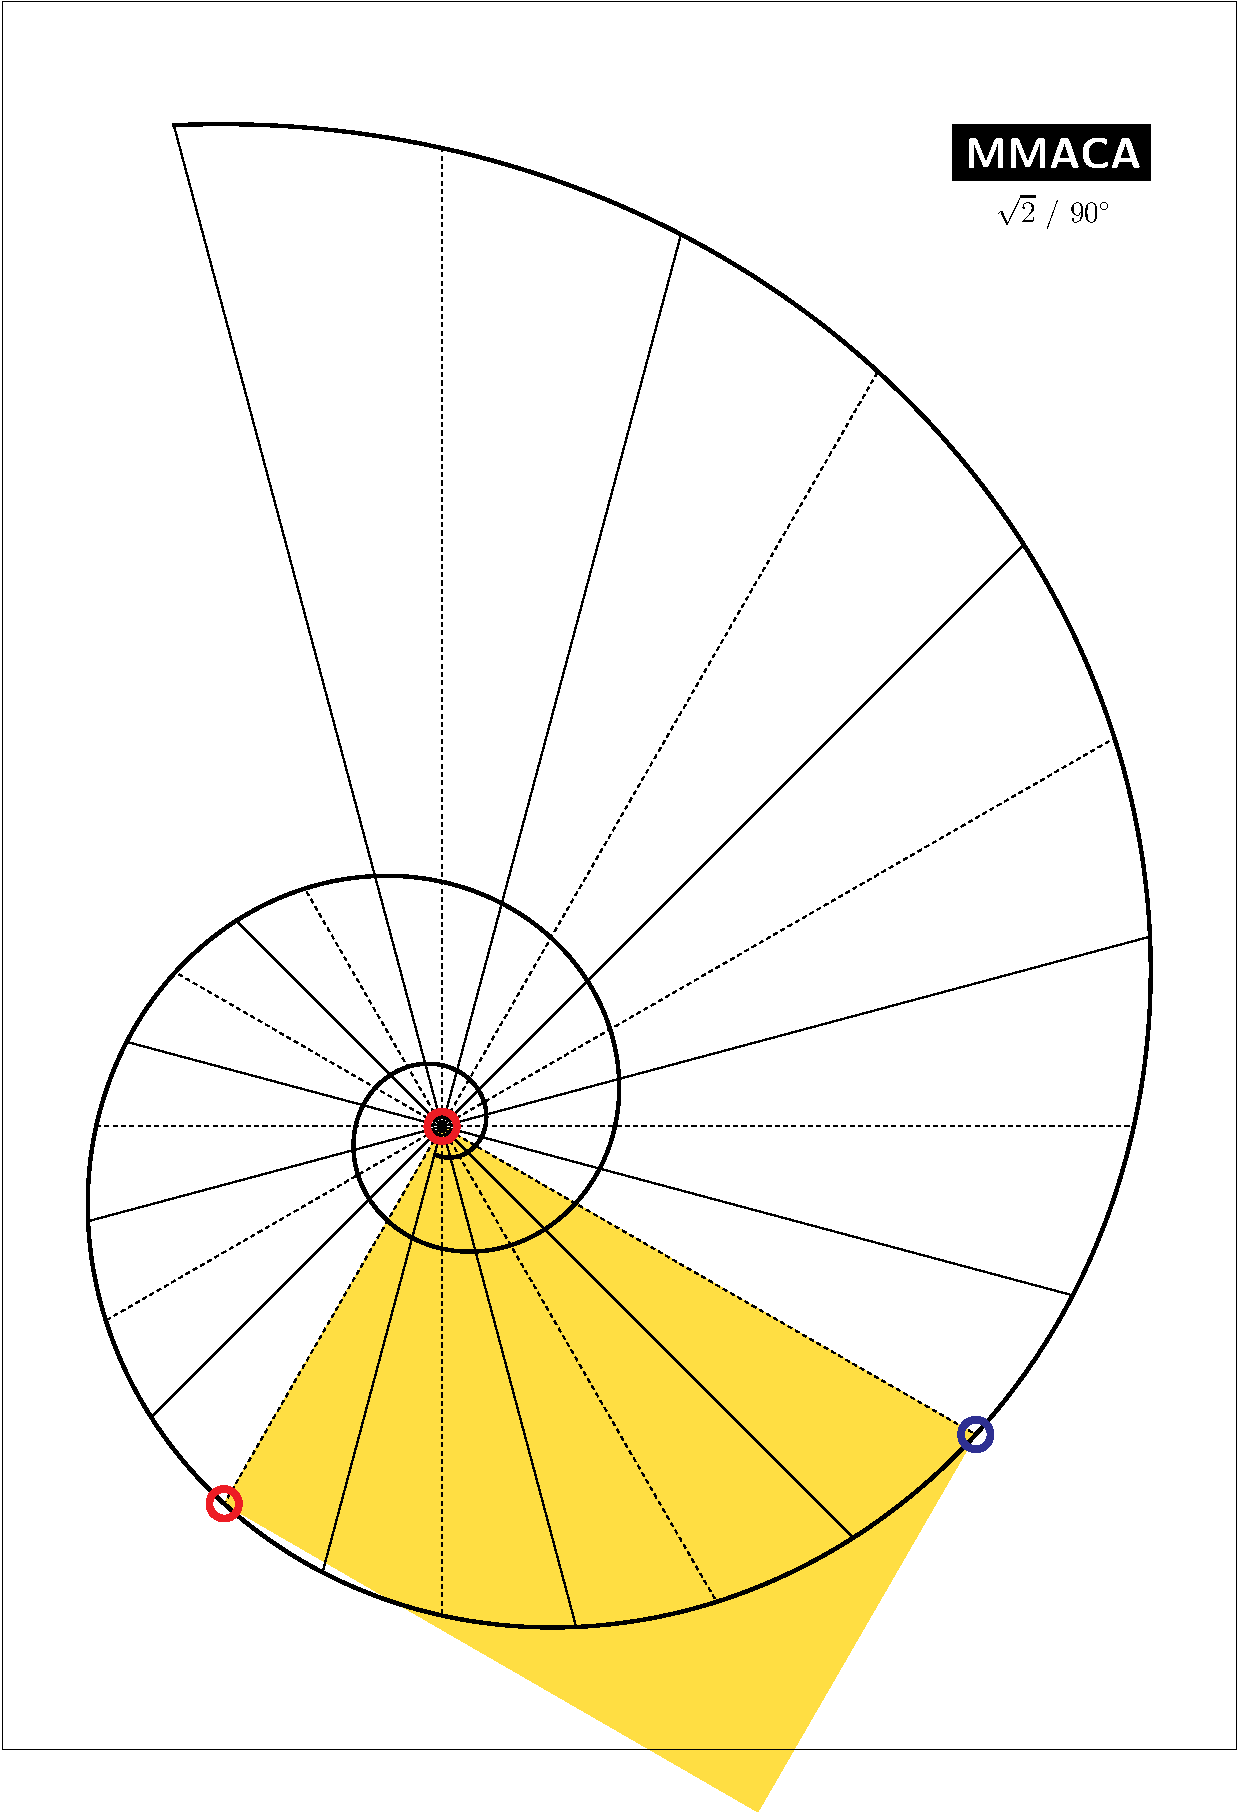
\includegraphics[scale=0.7071]{./pictures/Example_02}

    \end{center}

    \newpage

    %%%%%%%%%%%%%%%%%%%%%%%%%%%%%%%%%%%%%%%%%%%%%%%%%%%%%%%%%%%%%%%%%%%%%%%%%%%%

    \begin{center}
    
        \large

        Deduce the ratio of the sides of an A7 sheet of paper using the $\sqrt{2} \, / \, 270^{\circ}$ spiral

        \bigskip \bigskip \bigskip \bigskip
    
        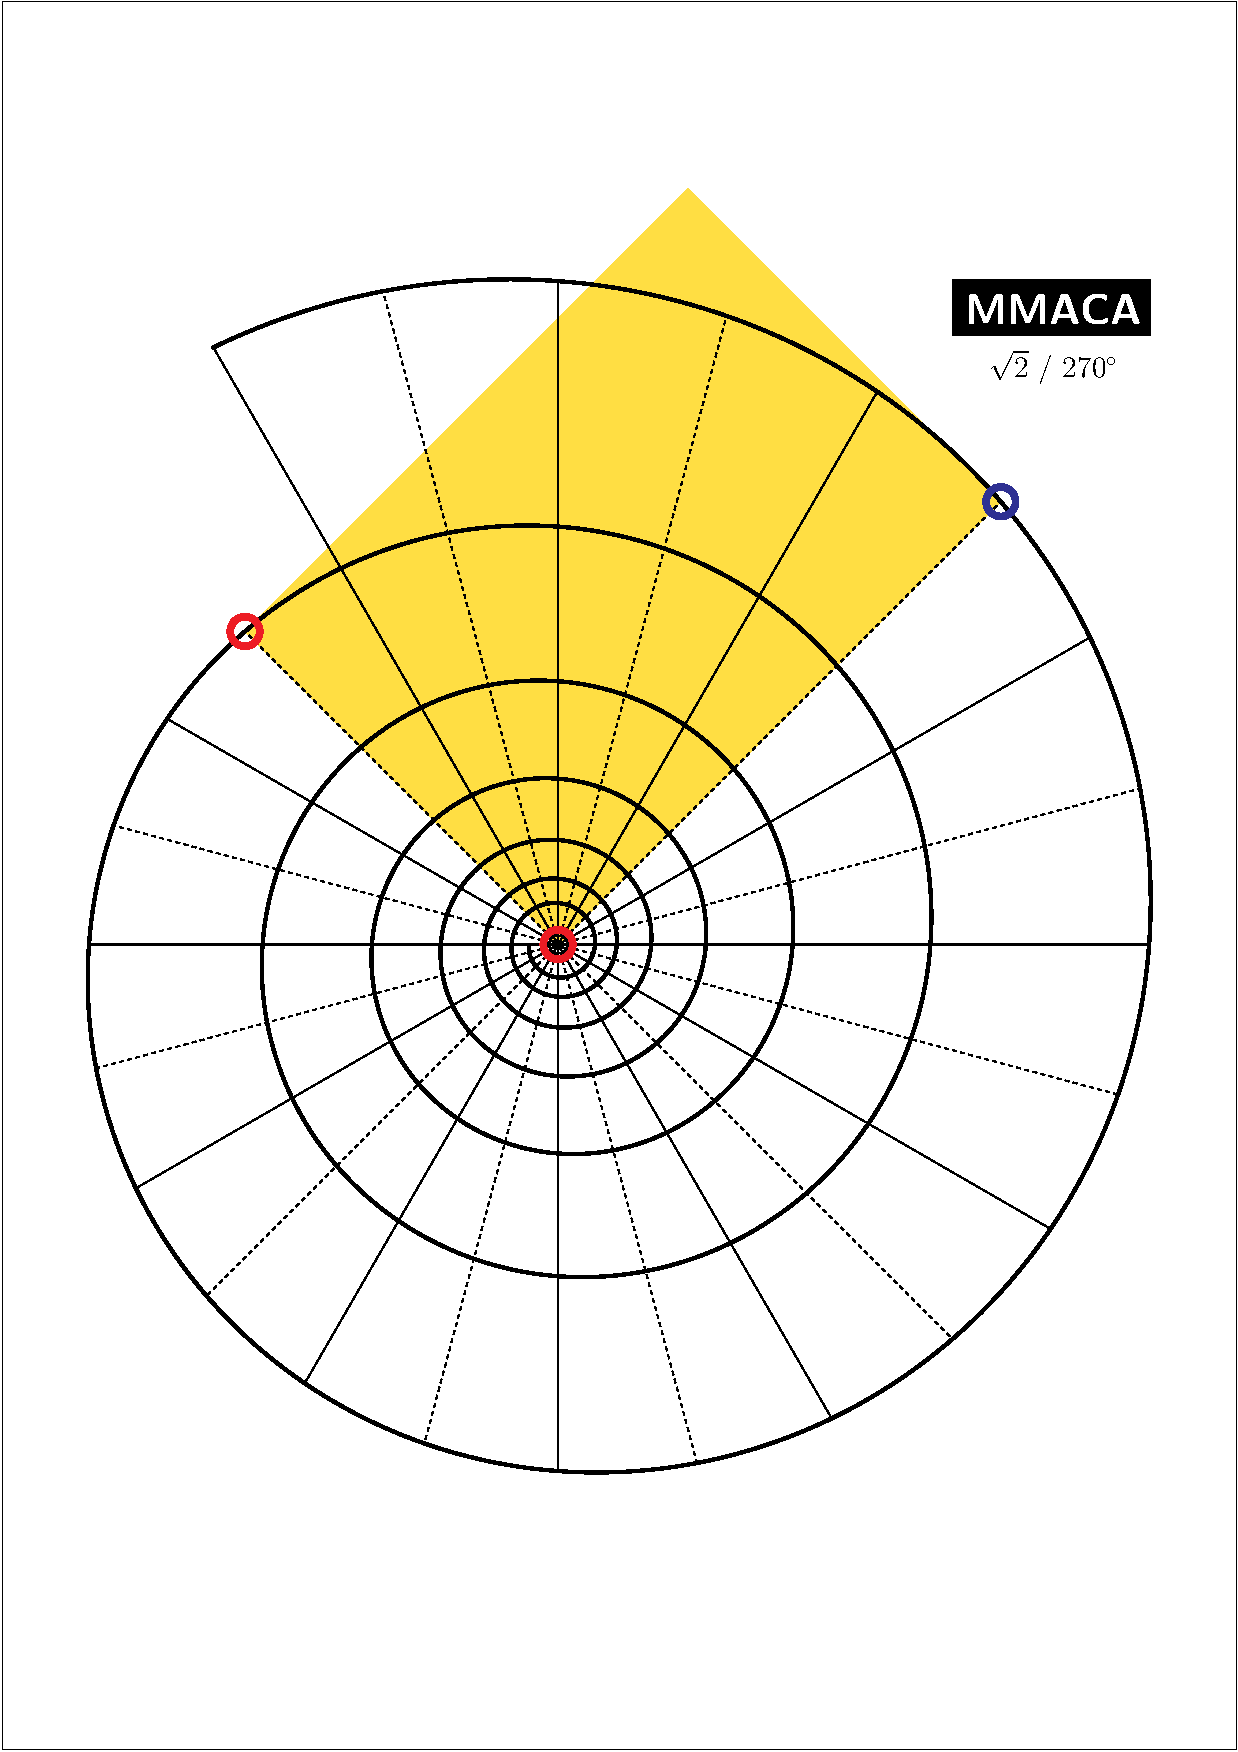
\includegraphics[scale=0.7071]{./pictures/Example_01}

    \end{center}

    \newpage

    %%%%%%%%%%%%%%%%%%%%%%%%%%%%%%%%%%%%%%%%%%%%%%%%%%%%%%%%%%%%%%%%%%%%%%%%%%%%

    \begin{center}
    
        \large

        Create a rectangle of $1\!:\!\sqrt{2}\;$ side ratio using the $4 \, / \, 360^{\circ}$ spiral

        \bigskip \bigskip \bigskip
    
        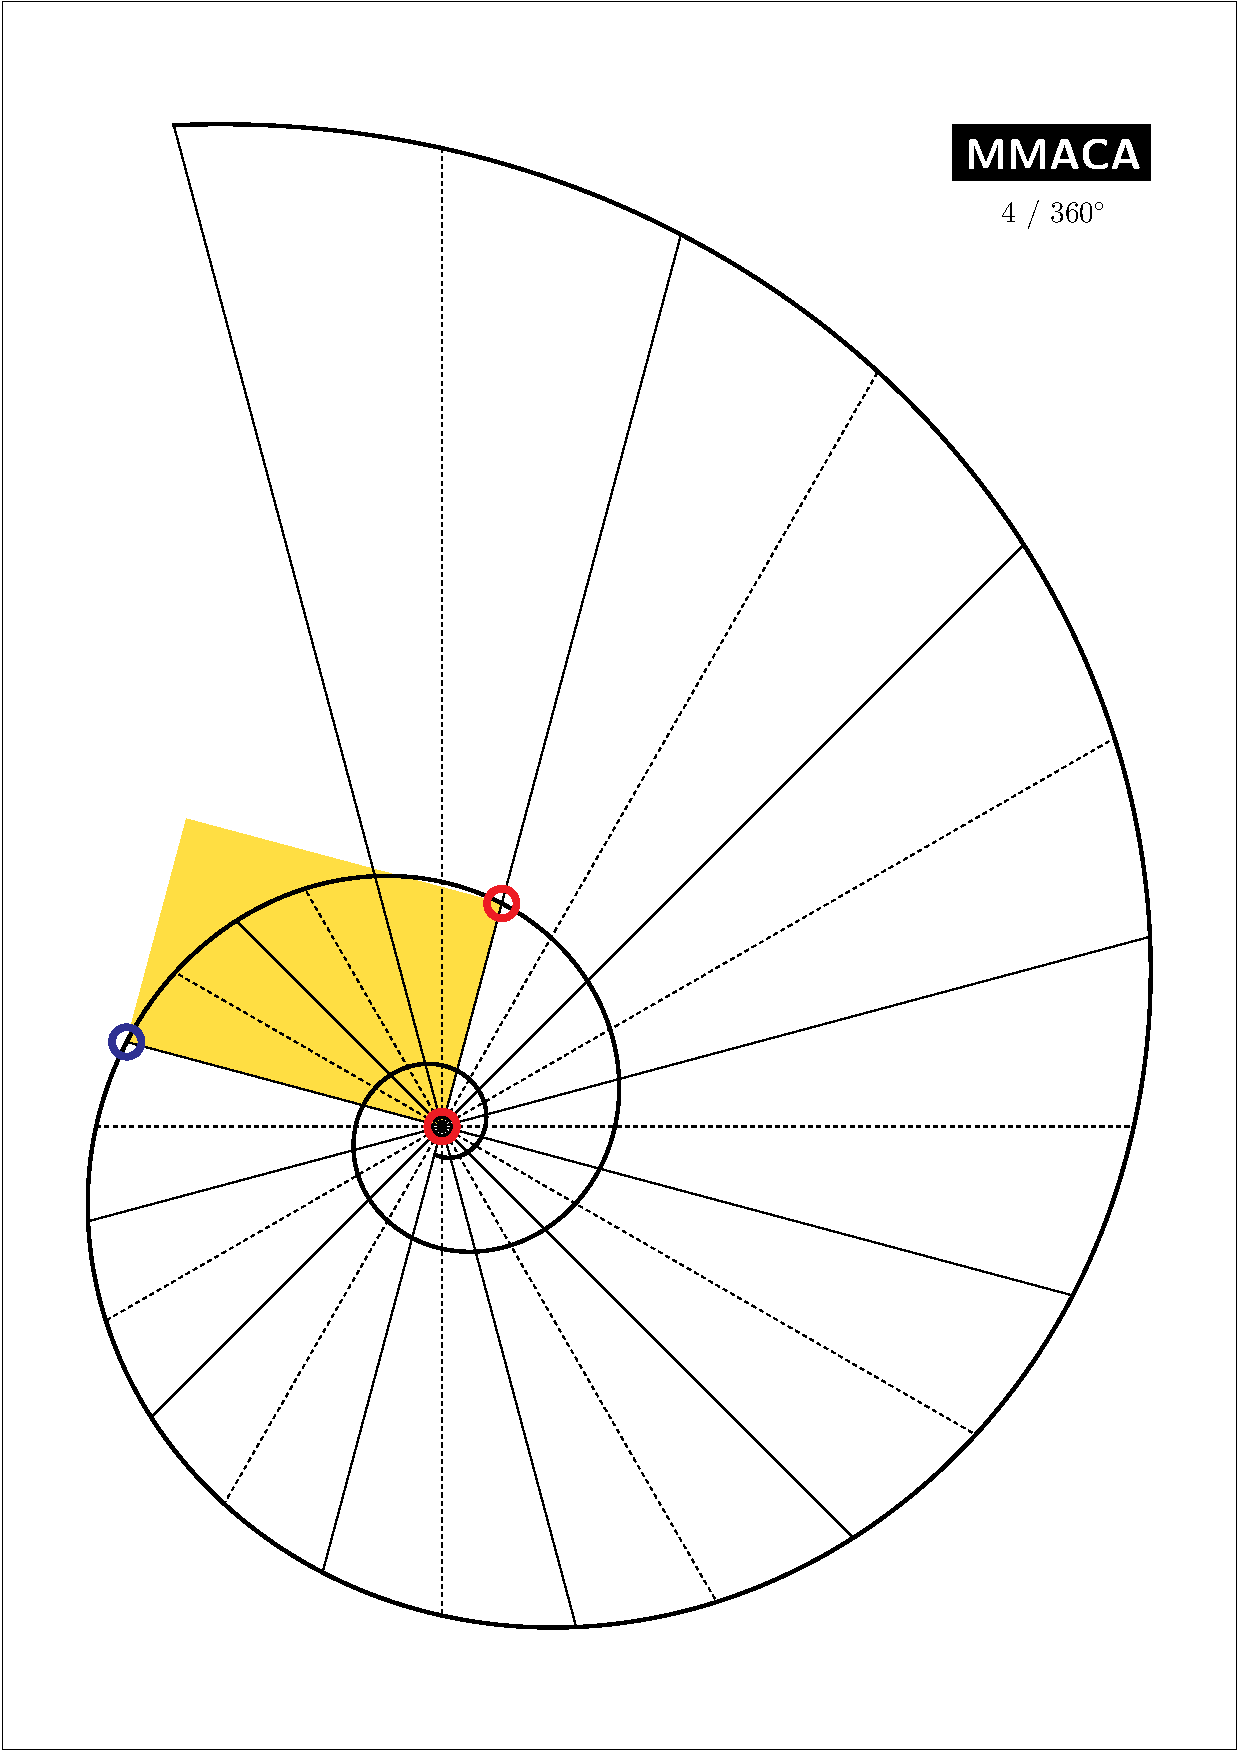
\includegraphics[scale=0.7071]{./pictures/Example_05}

    \end{center}

    \newpage

    %%%%%%%%%%%%%%%%%%%%%%%%%%%%%%%%%%%%%%%%%%%%%%%%%%%%%%%%%%%%%%%%%%%%%%%%%%%%

    \begin{center}
    
        \large

        Determine the side / diagonal length ratio of a square using the $2 \, / \, 90^{\circ}$ spiral

        \bigskip \bigskip \bigskip
    
        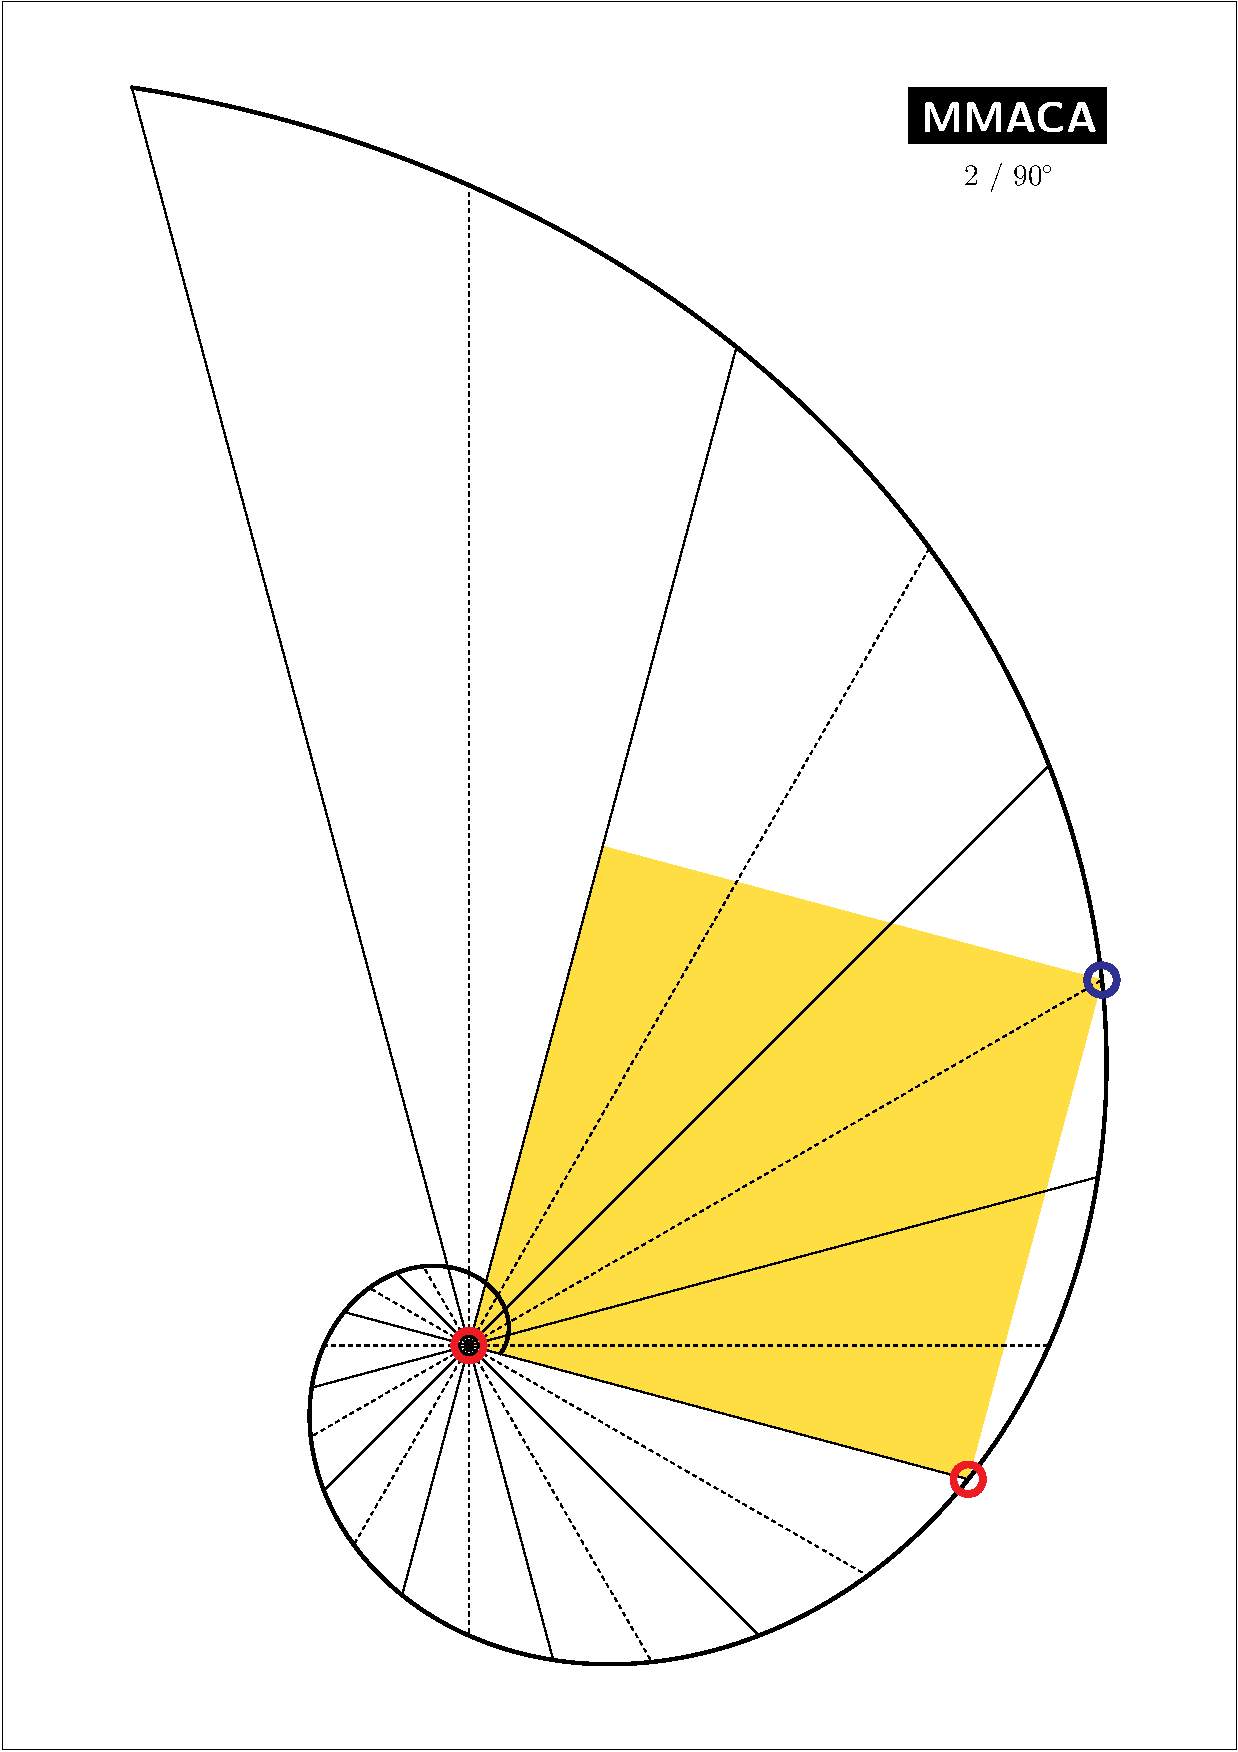
\includegraphics[scale=0.7071]{./pictures/Example_07}

    \end{center}

    \newpage

    %%%%%%%%%%%%%%%%%%%%%%%%%%%%%%%%%%%%%%%%%%%%%%%%%%%%%%%%%%%%%%%%%%%%%%%%%%%%

    \begin{center}
    
        \large

        Determine leg length ratio of a $30^{\circ}$\,-\,$60^{\circ}$\,-\,$90^{\circ}$ triangle using the $\sqrt{3} \, / \, 270^{\circ}$ spiral

        \bigskip \bigskip \bigskip
    
        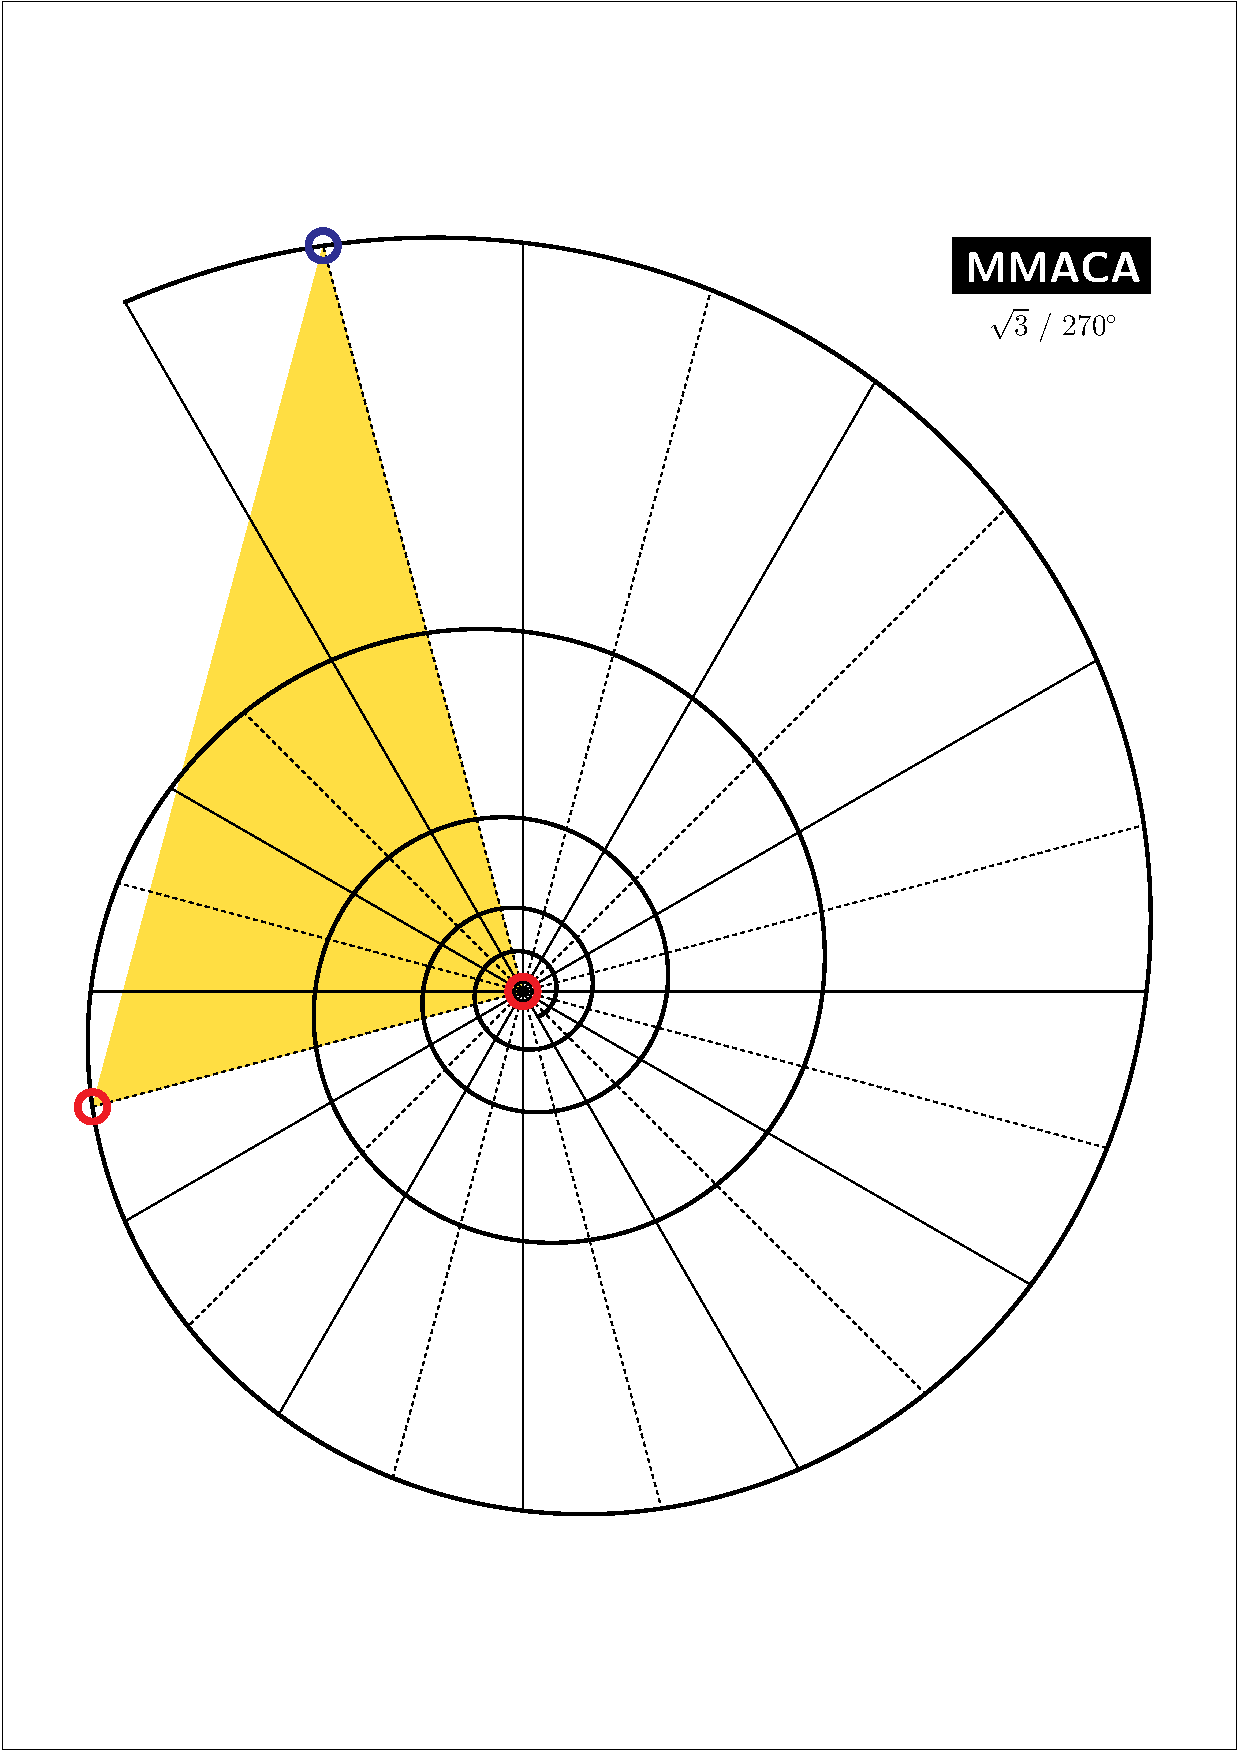
\includegraphics[scale=0.7071]{./pictures/Example_06}

    \end{center}

    \newpage

    %%%%%%%%%%%%%%%%%%%%%%%%%%%%%%%%%%%%%%%%%%%%%%%%%%%%%%%%%%%%%%%%%%%%%%%%%%%%

    \begin{center}
    
        \large

        Verify that credit cards are usually golden rectangles using the $\phi \, / \, 270^{\circ}$ spiral

        \bigskip \bigskip \bigskip
    
        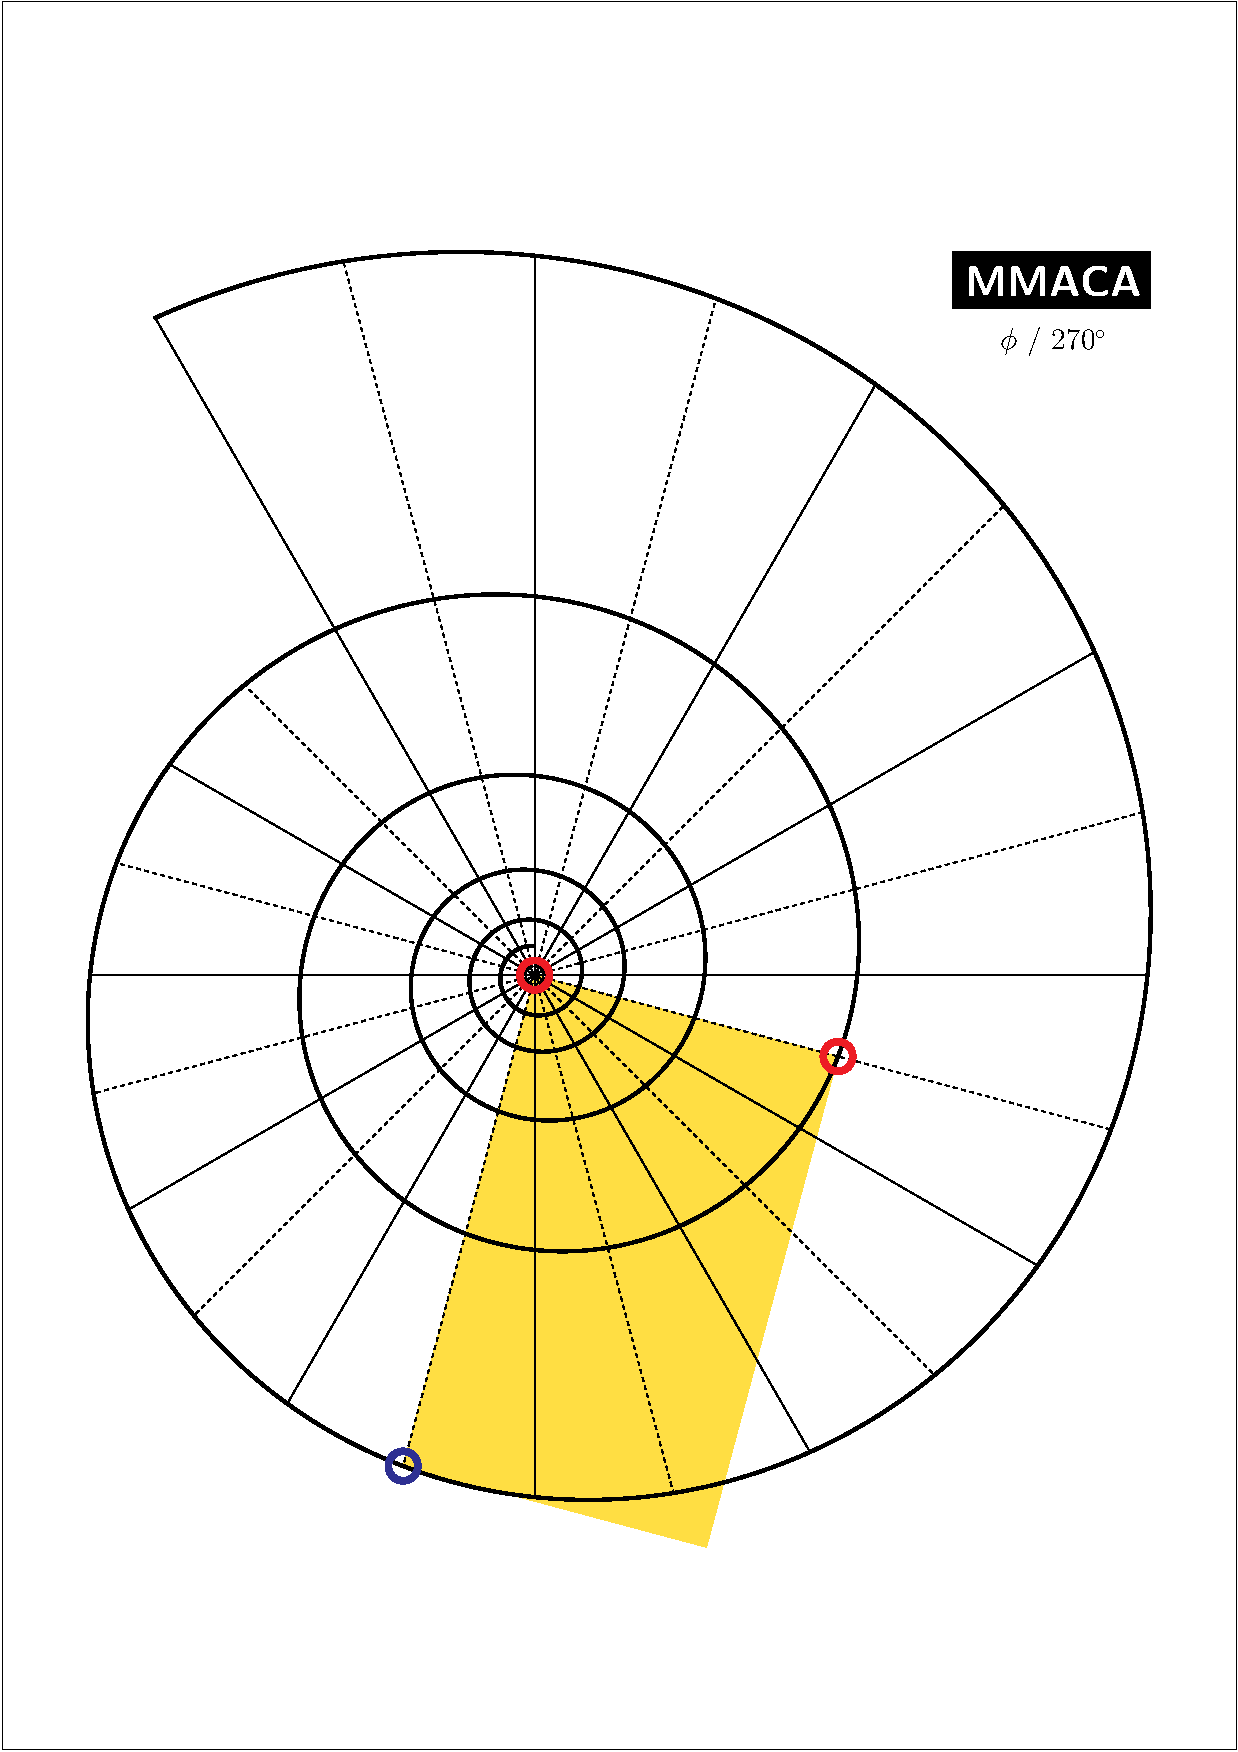
\includegraphics[scale=0.7071]{./pictures/Example_08}

    \end{center}

    \newpage

    %%%%%%%%%%%%%%%%%%%%%%%%%%%%%%%%%%%%%%%%%%%%%%%%%%%%%%%%%%%%%%%%%%%%%%%%%%%%

    \begin{center}
    
        \large

        Divide a segment by the golden ratio using the $\phi \, / \, 360^{\circ}$ spiral

        \bigskip \bigskip \bigskip
    
        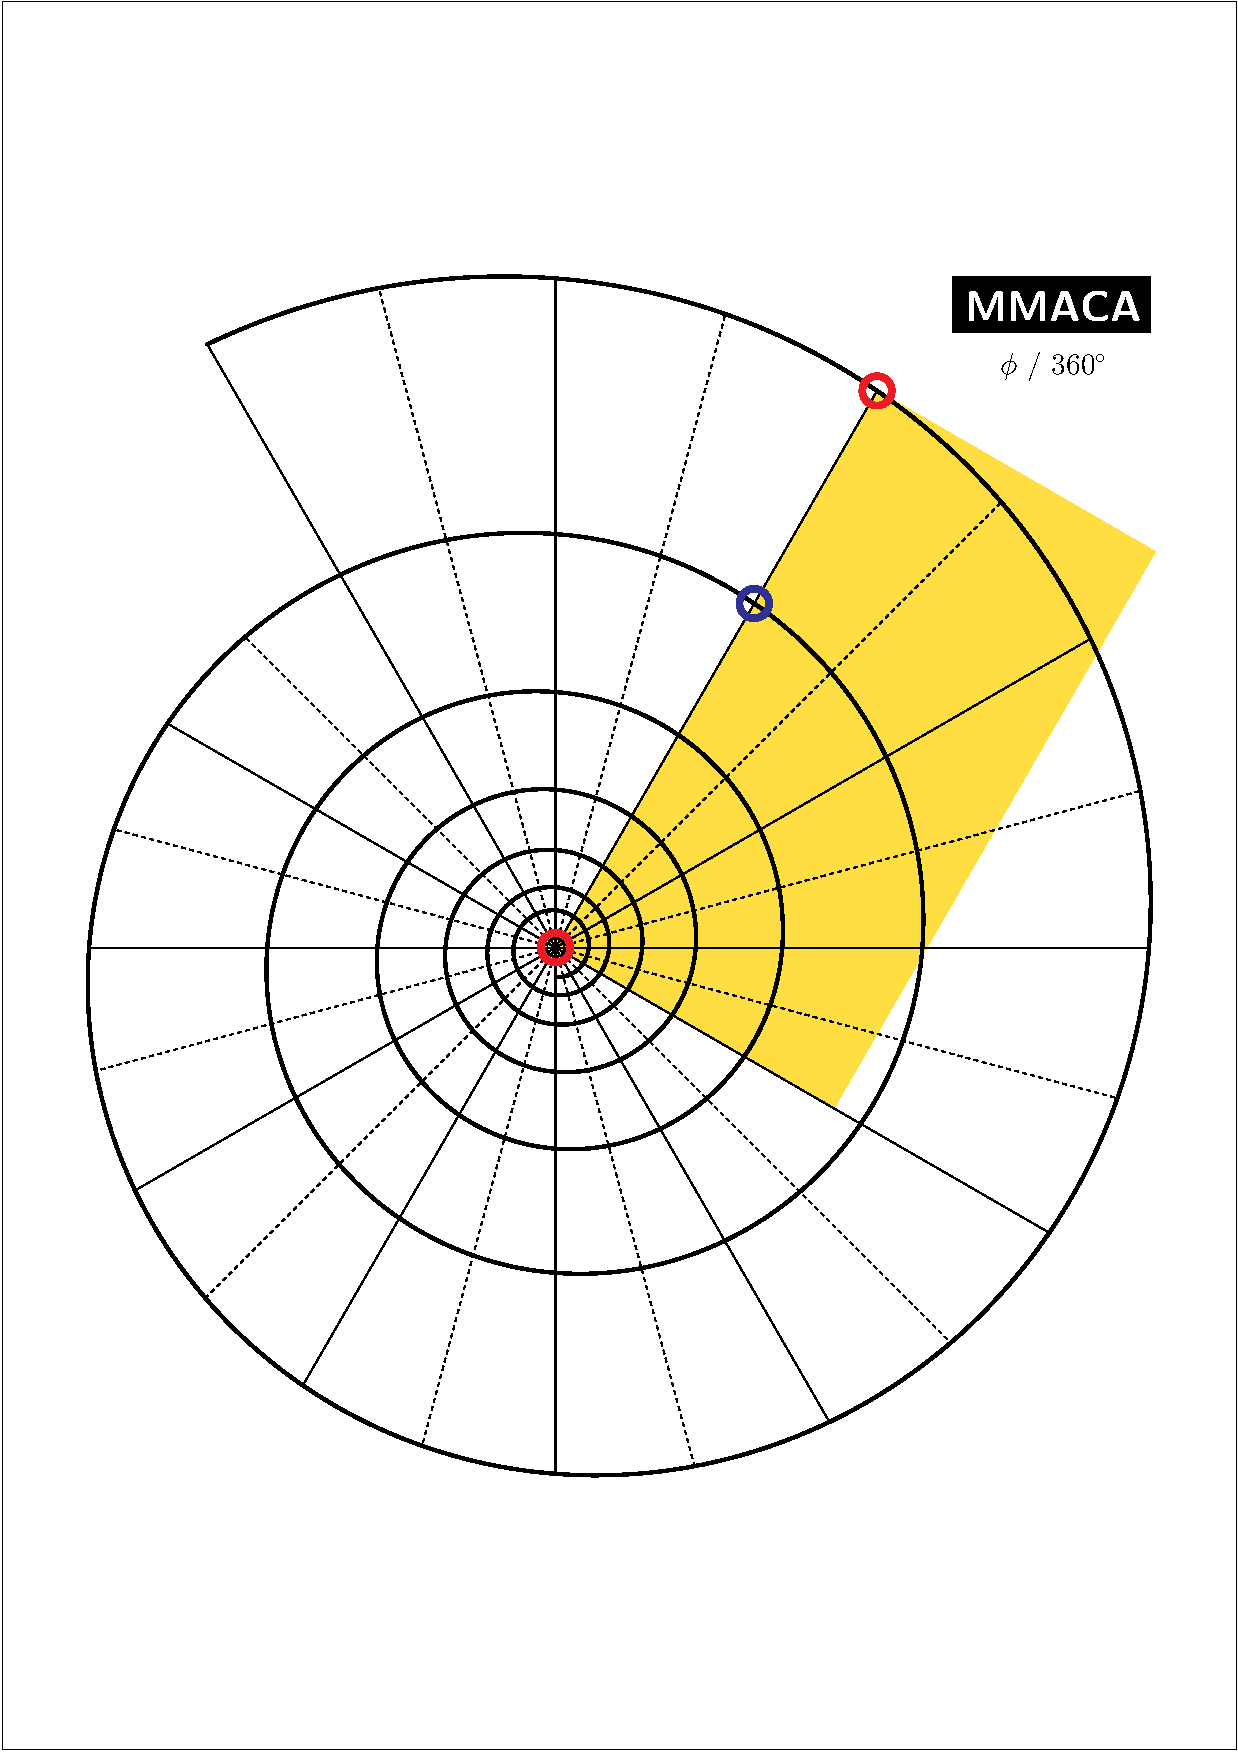
\includegraphics[scale=0.7071]{./pictures/Example_09}

    \end{center}

    \newpage

    %%%%%%%%%%%%%%%%%%%%%%%%%%%%%%%%%%%%%%%%%%%%%%%%%%%%%%%%%%%%%%%%%%%%%%%%%%%%

    \begin{center}
    
        \large

        Divide a segment by the golden ratio using the $\phi \, / \, 180^{\circ}$ spiral

        \bigskip \bigskip \bigskip
    
        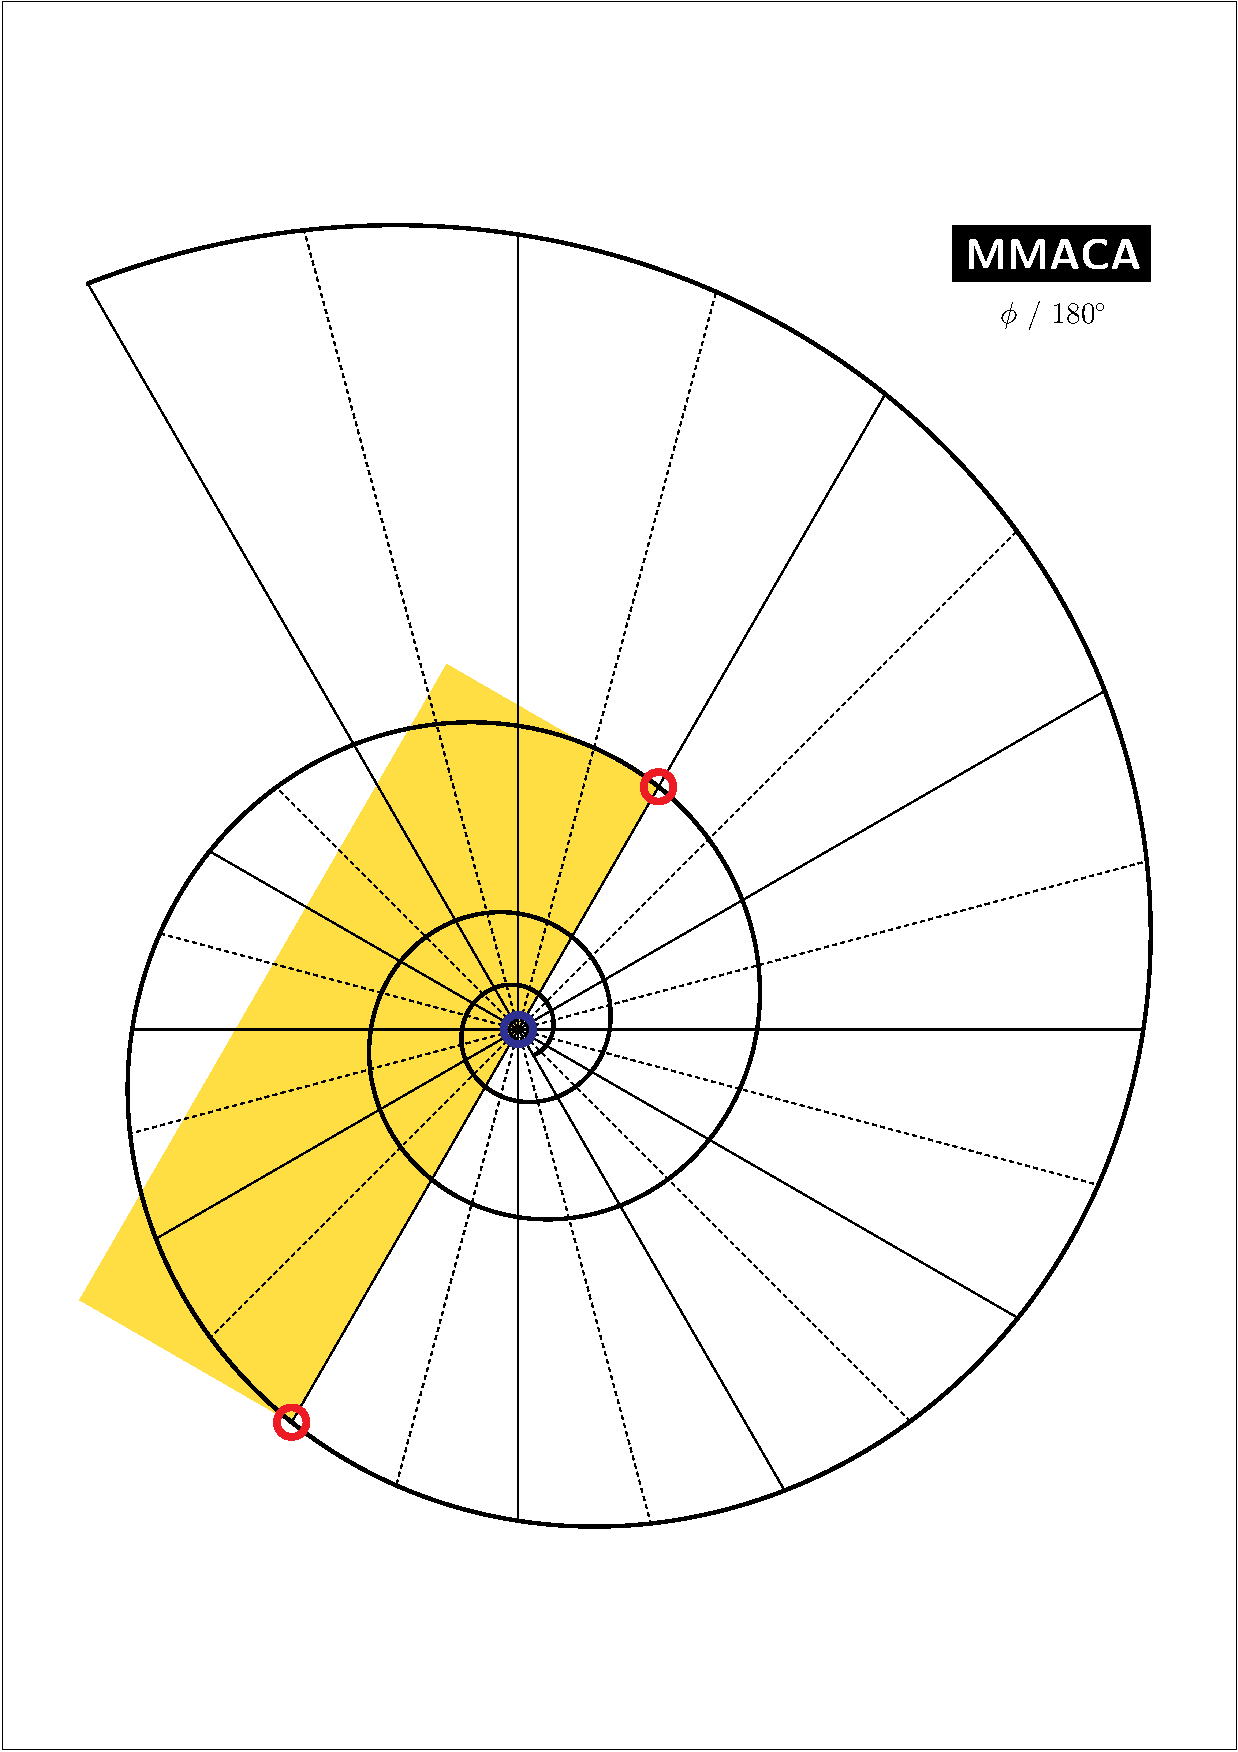
\includegraphics[scale=0.7071]{./pictures/Example_10}

    \end{center}

    \newpage

    %%%%%%%%%%%%%%%%%%%%%%%%%%%%%%%%%%%%%%%%%%%%%%%%%%%%%%%%%%%%%%%%%%%%%%%%%%%%

    \begin{center}
    
        \large

        Verify that the Fibonacci spiral is a good approximation of the $\phi \, / \, 90^{\circ}$ spiral

        \bigskip \bigskip \bigskip
    
        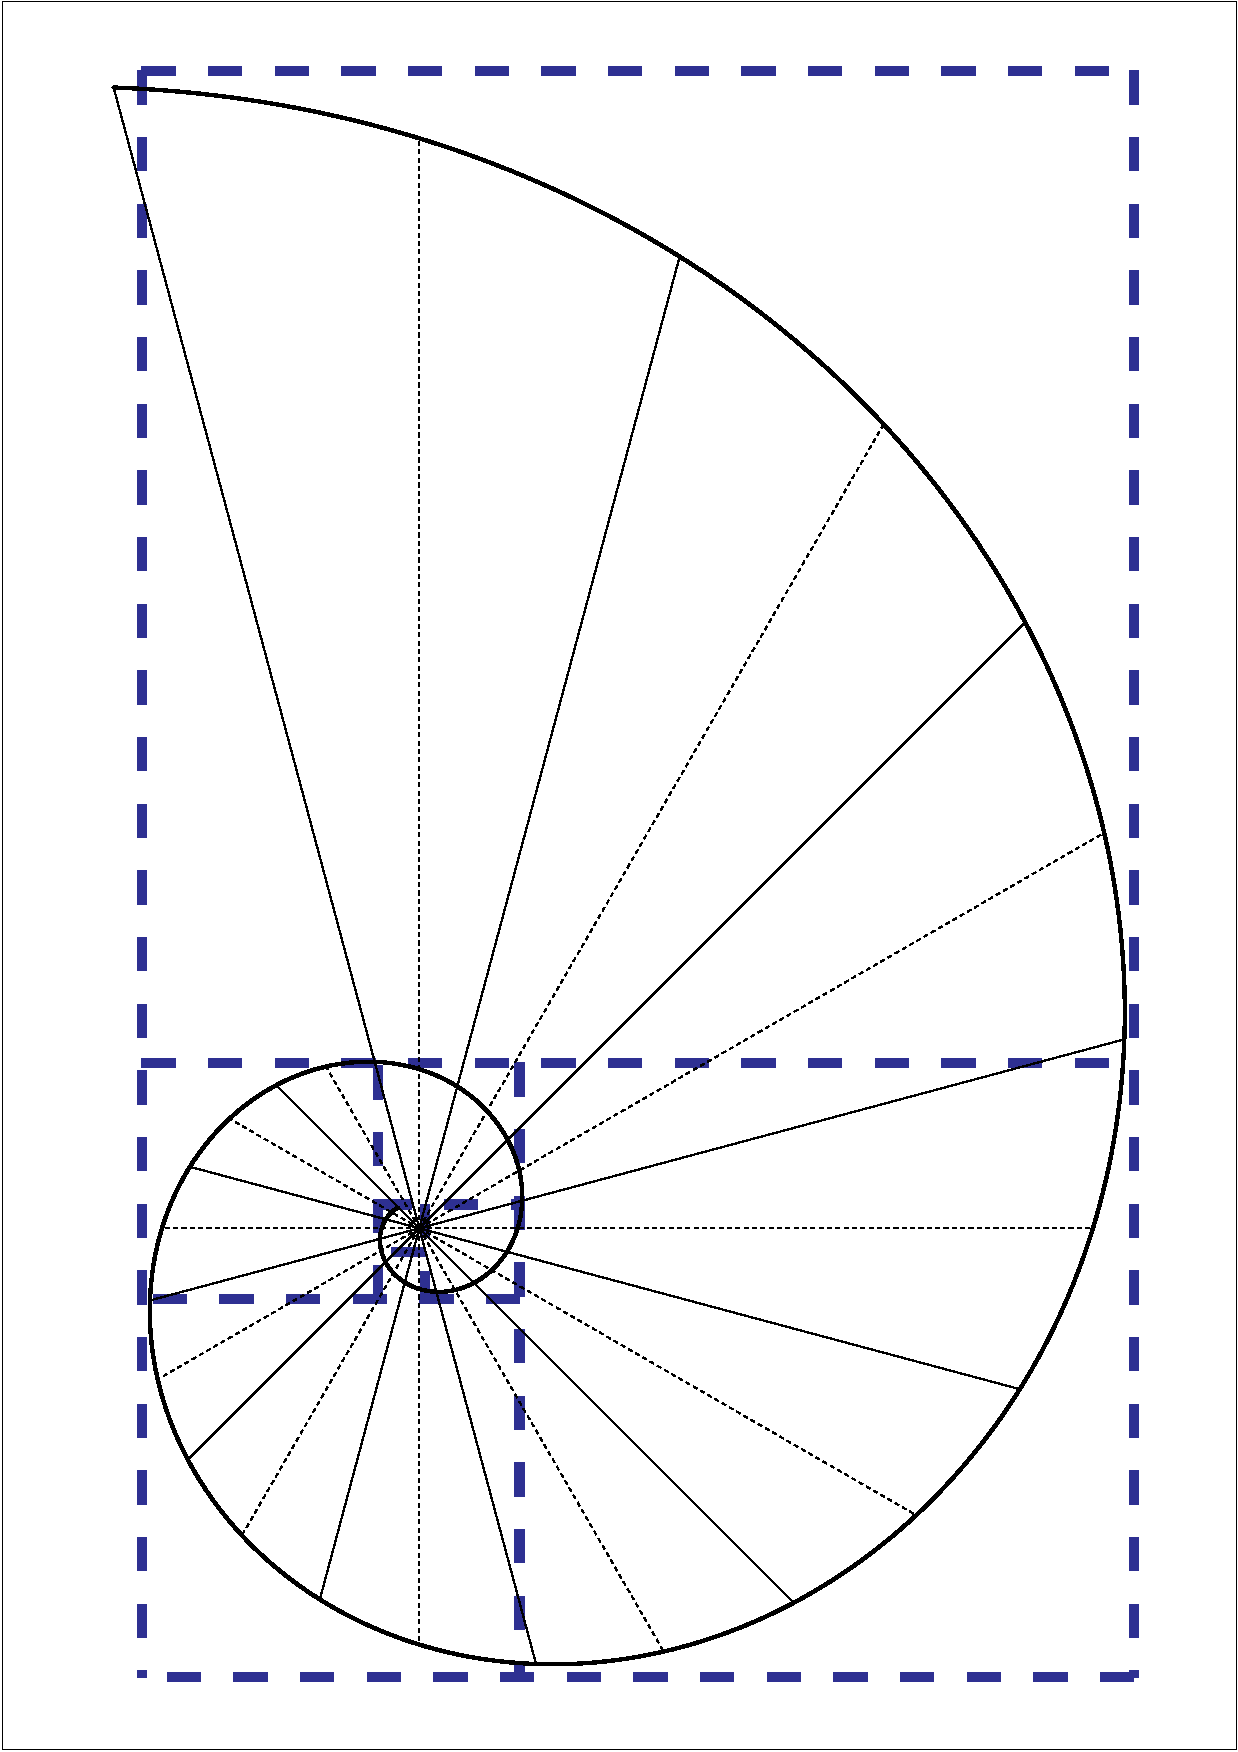
\includegraphics[scale=0.7071]{./pictures/Example_11b}

    \end{center}

    \newpage

    %%%%%%%%%%%%%%%%%%%%%%%%%%%%%%%%%%%%%%%%%%%%%%%%%%%%%%%%%%%%%%%%%%%%%%%%%%%%

    \begin{center}
    
        \large

        Explain why the $4 \, / \, 360^{\circ}$, the $2 \, / \, 180^{\circ}$ and the $\sqrt{2} \, / \, 90^{\circ}$ spirals are equal

        \bigskip \bigskip \bigskip
    
        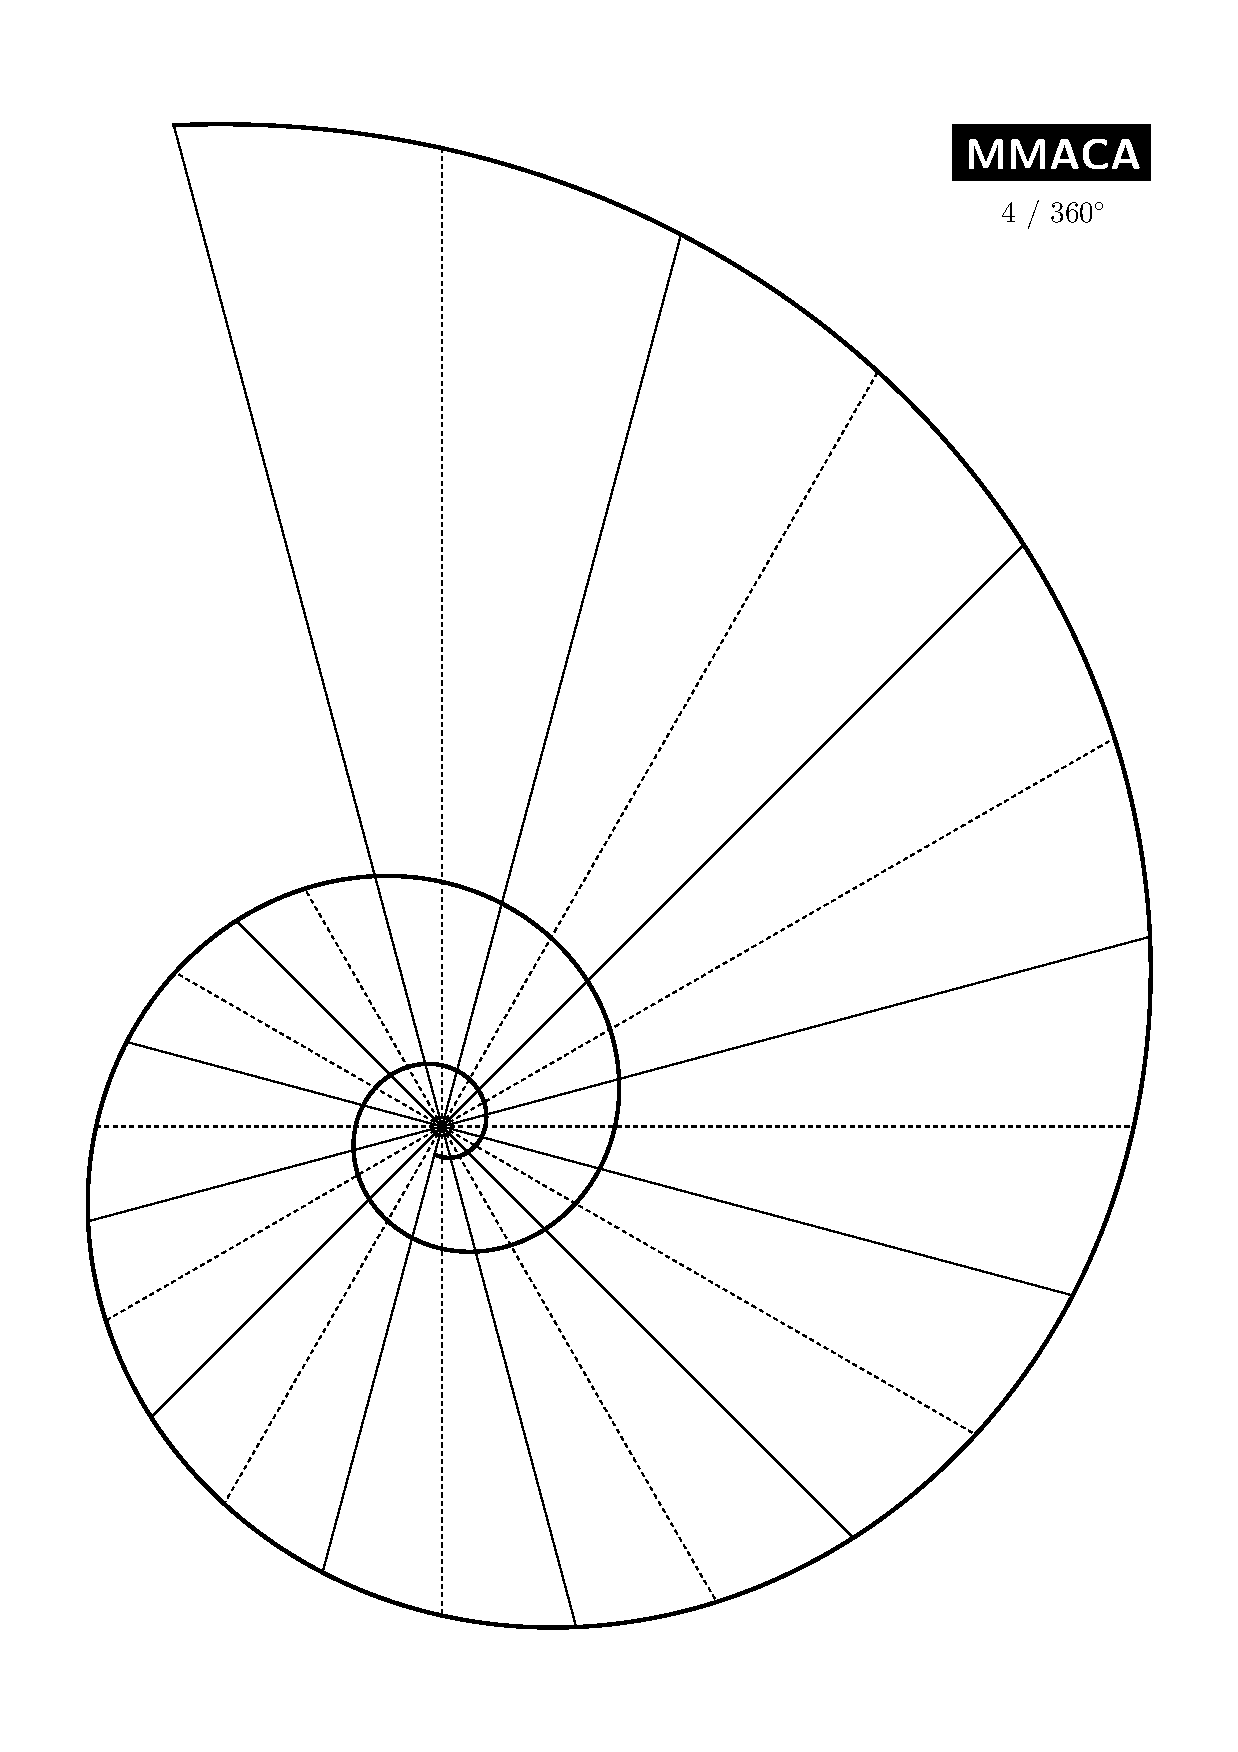
\includegraphics[scale=0.3535]{./pictures/Spiral_4_360}
        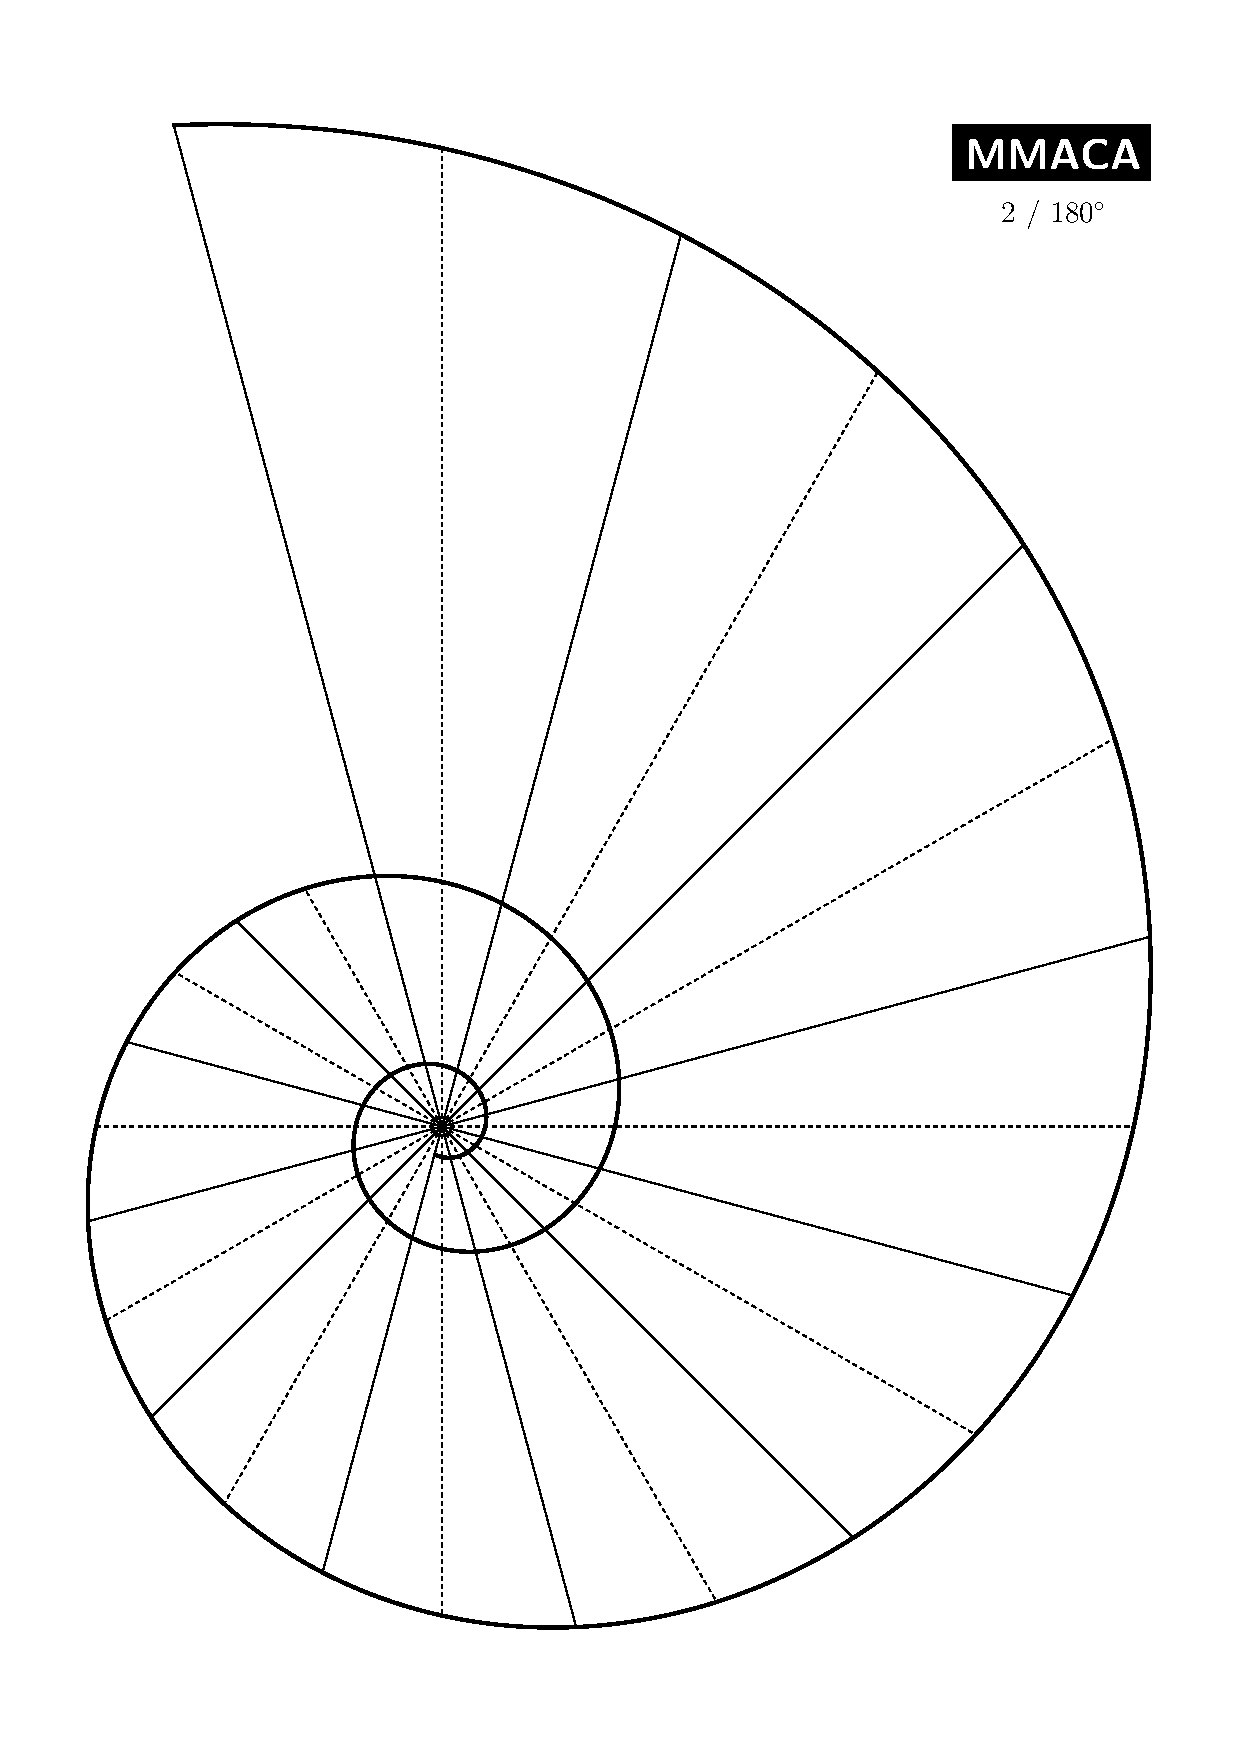
\includegraphics[scale=0.3535]{./pictures/Spiral_2_180}
        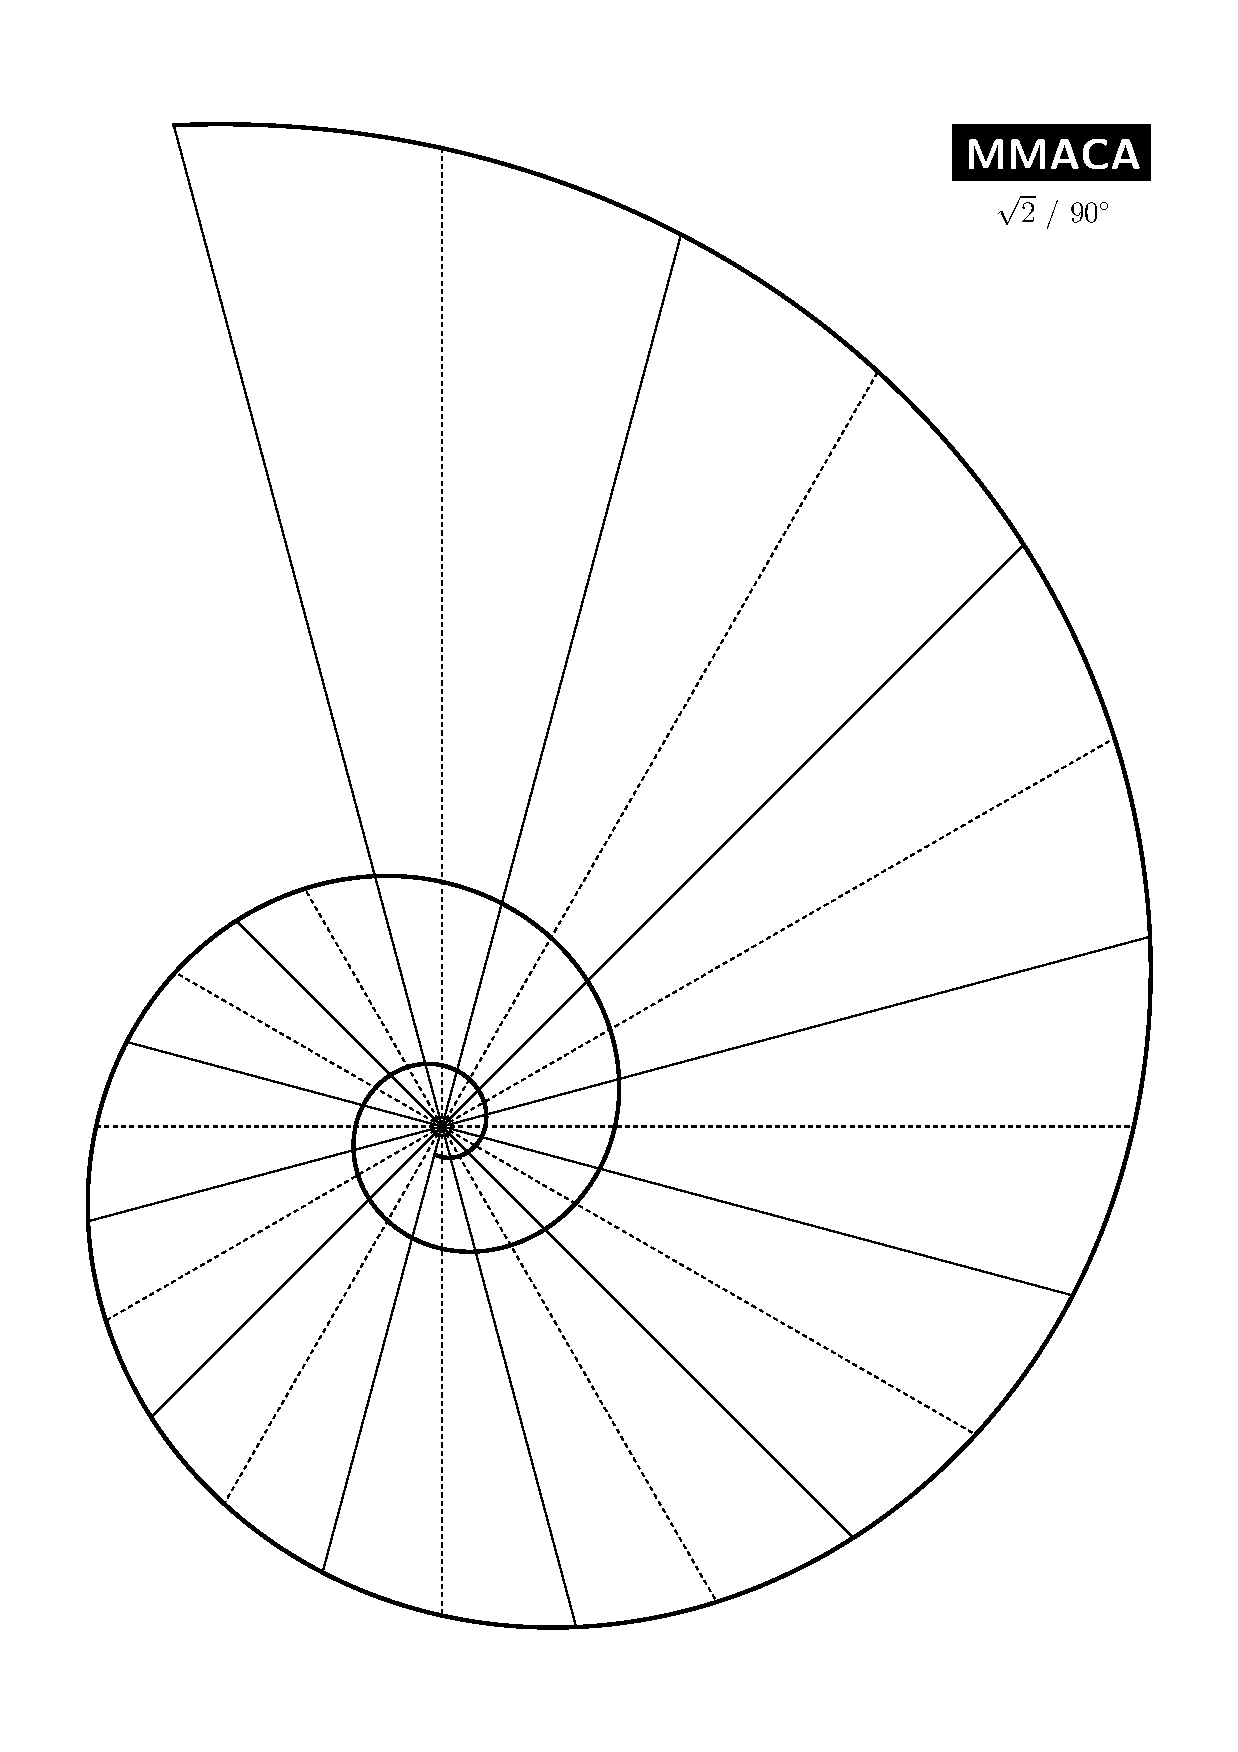
\includegraphics[scale=0.3535]{./pictures/Spiral_Root2_090}

        \bigskip \bigskip

        Determine the multiplicative constant $\lambda$ associated with each of the 24 angles



    \end{center}

    \newpage

    %%%%%%%%%%%%%%%%%%%%%%%%%%%%%%%%%%%%%%%%%%%%%%%%%%%%%%%%%%%%%%%%%%%%%%%%%%%%

    \begin{center}
    
        \large

        Explain how the $2 \, / \, 270^{\circ}$ spiral can be used to solve the «Delian problem»

        \bigskip \bigskip \bigskip
    
        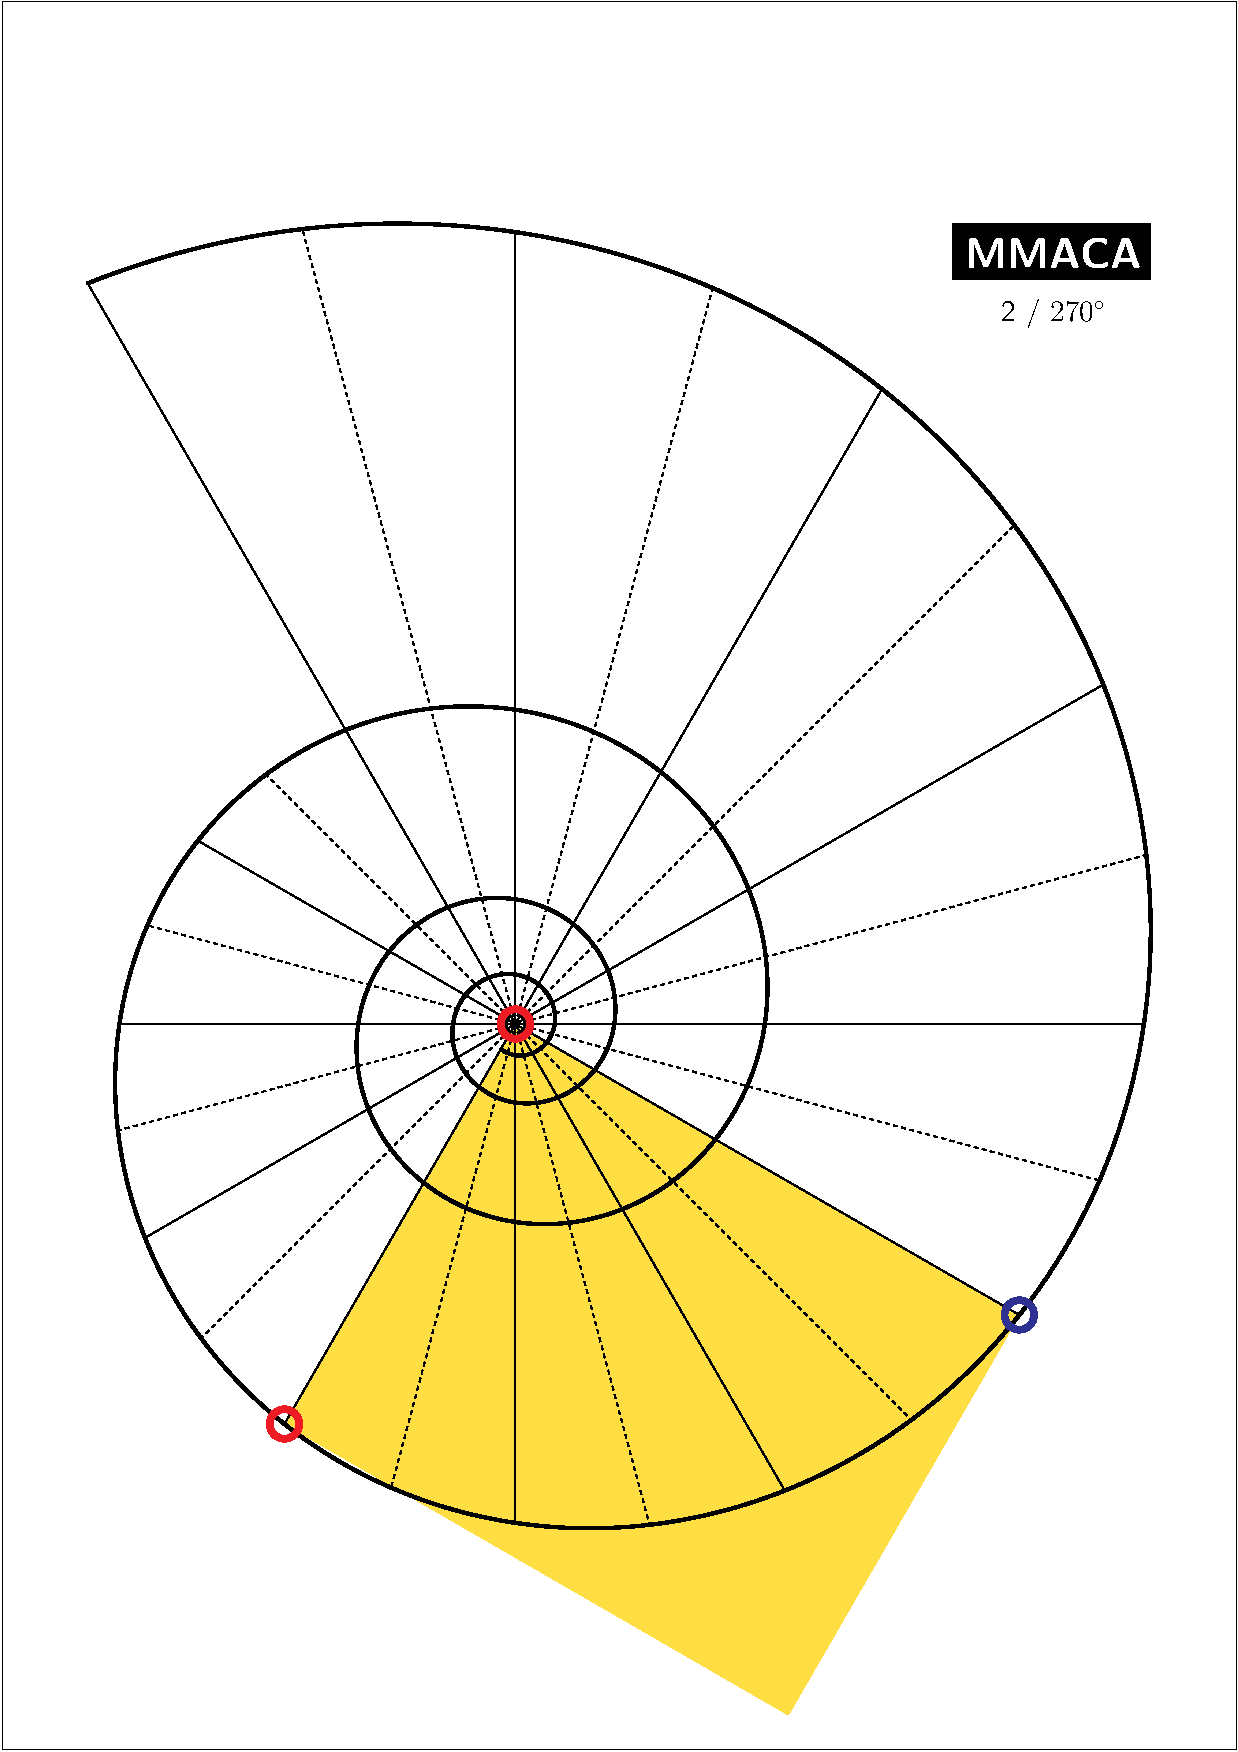
\includegraphics[scale=0.7071]{./pictures/Example_15}

    \end{center}

    \newpage

    %%%%%%%%%%%%%%%%%%%%%%%%%%%%%%%%%%%%%%%%%%%%%%%%%%%%%%%%%%%%%%%%%%%%%%%%%%%%

    \phantom{.}
    \vspace{26em}

    {\huge \bf Spira Mirabilis templates}

    \bigskip

    {\large A curated set of printable templates for educational purposes}

    \newpage

    %%% TEMPLATES %%%%%%%%%%%%%%%%%%%%%%%%%%%%%%%%%%%%%%%%%%%%%%%%%%%%%%%%%%%%%%

    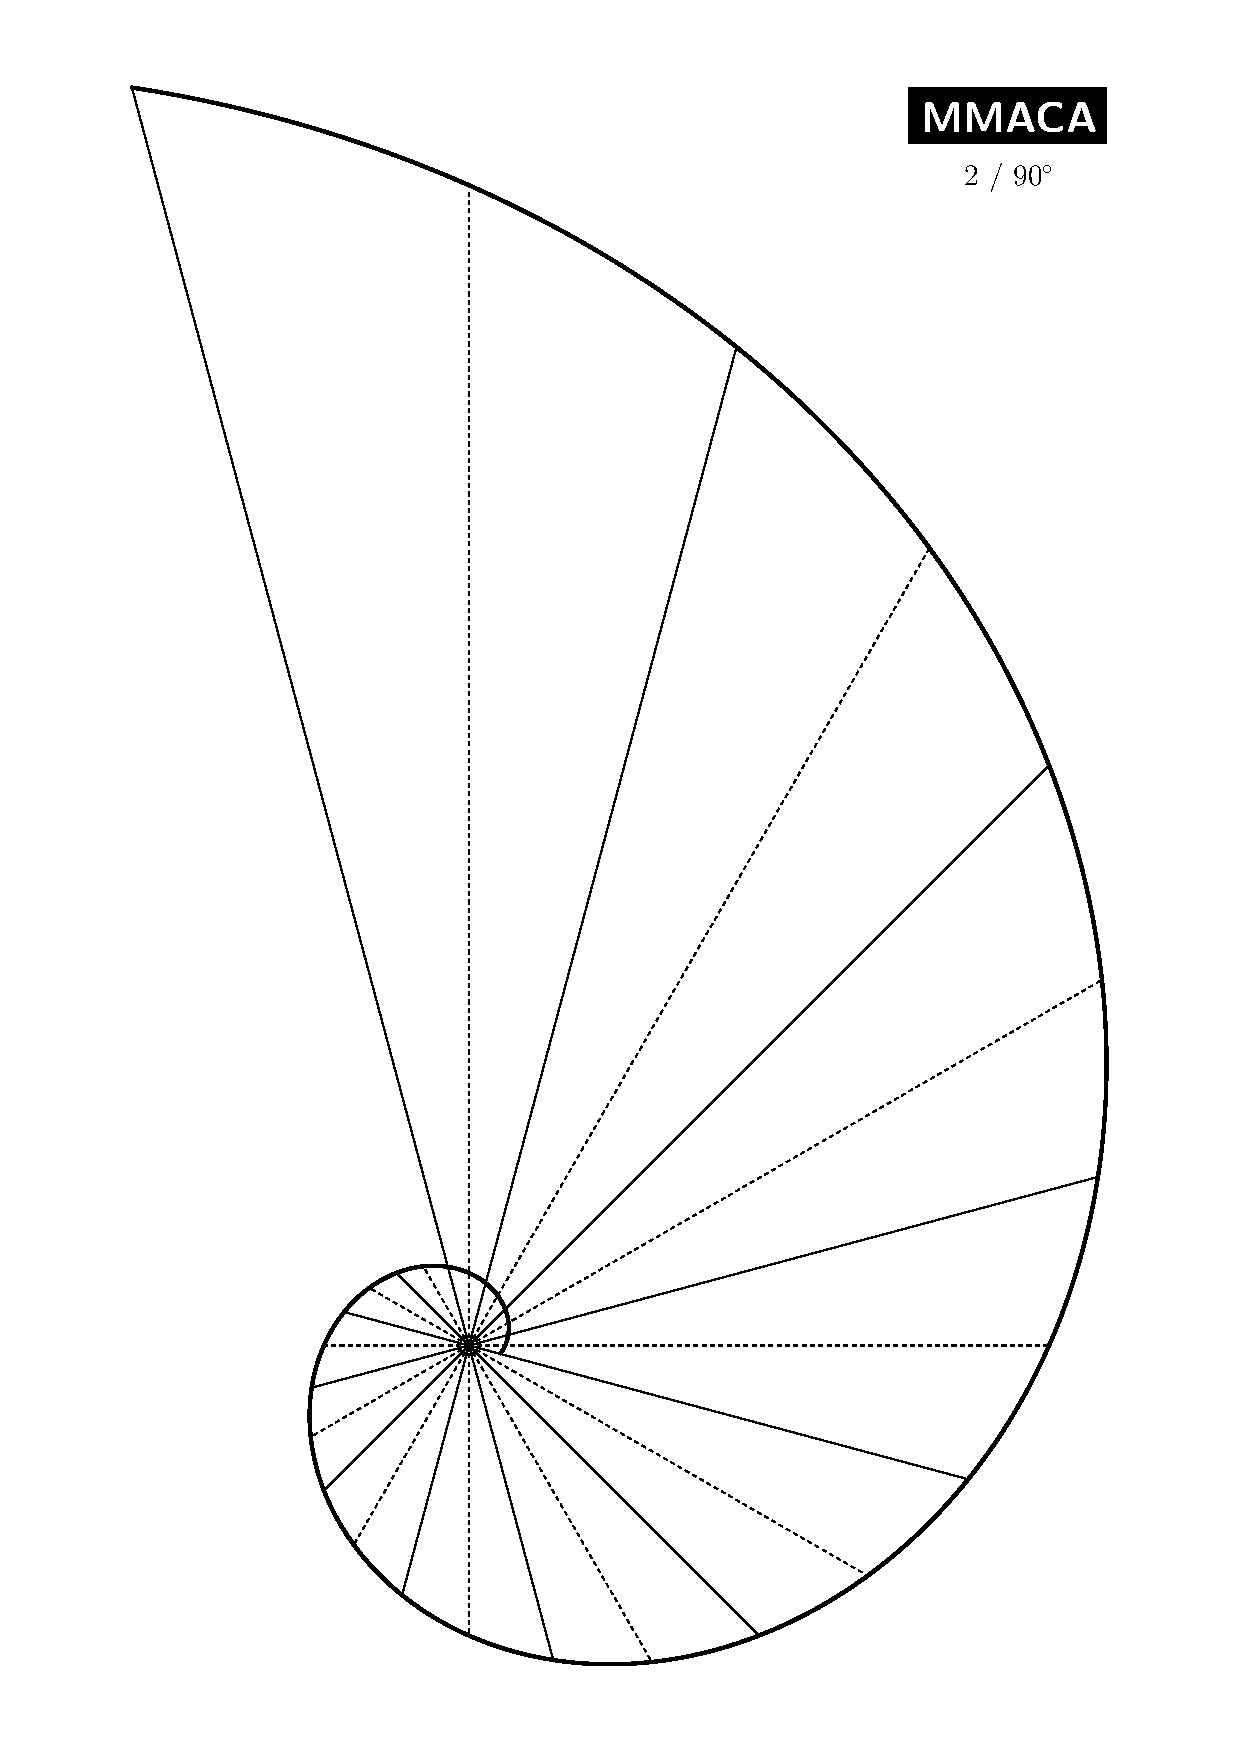
\includepdf{./pictures/Spiral_2_090}
    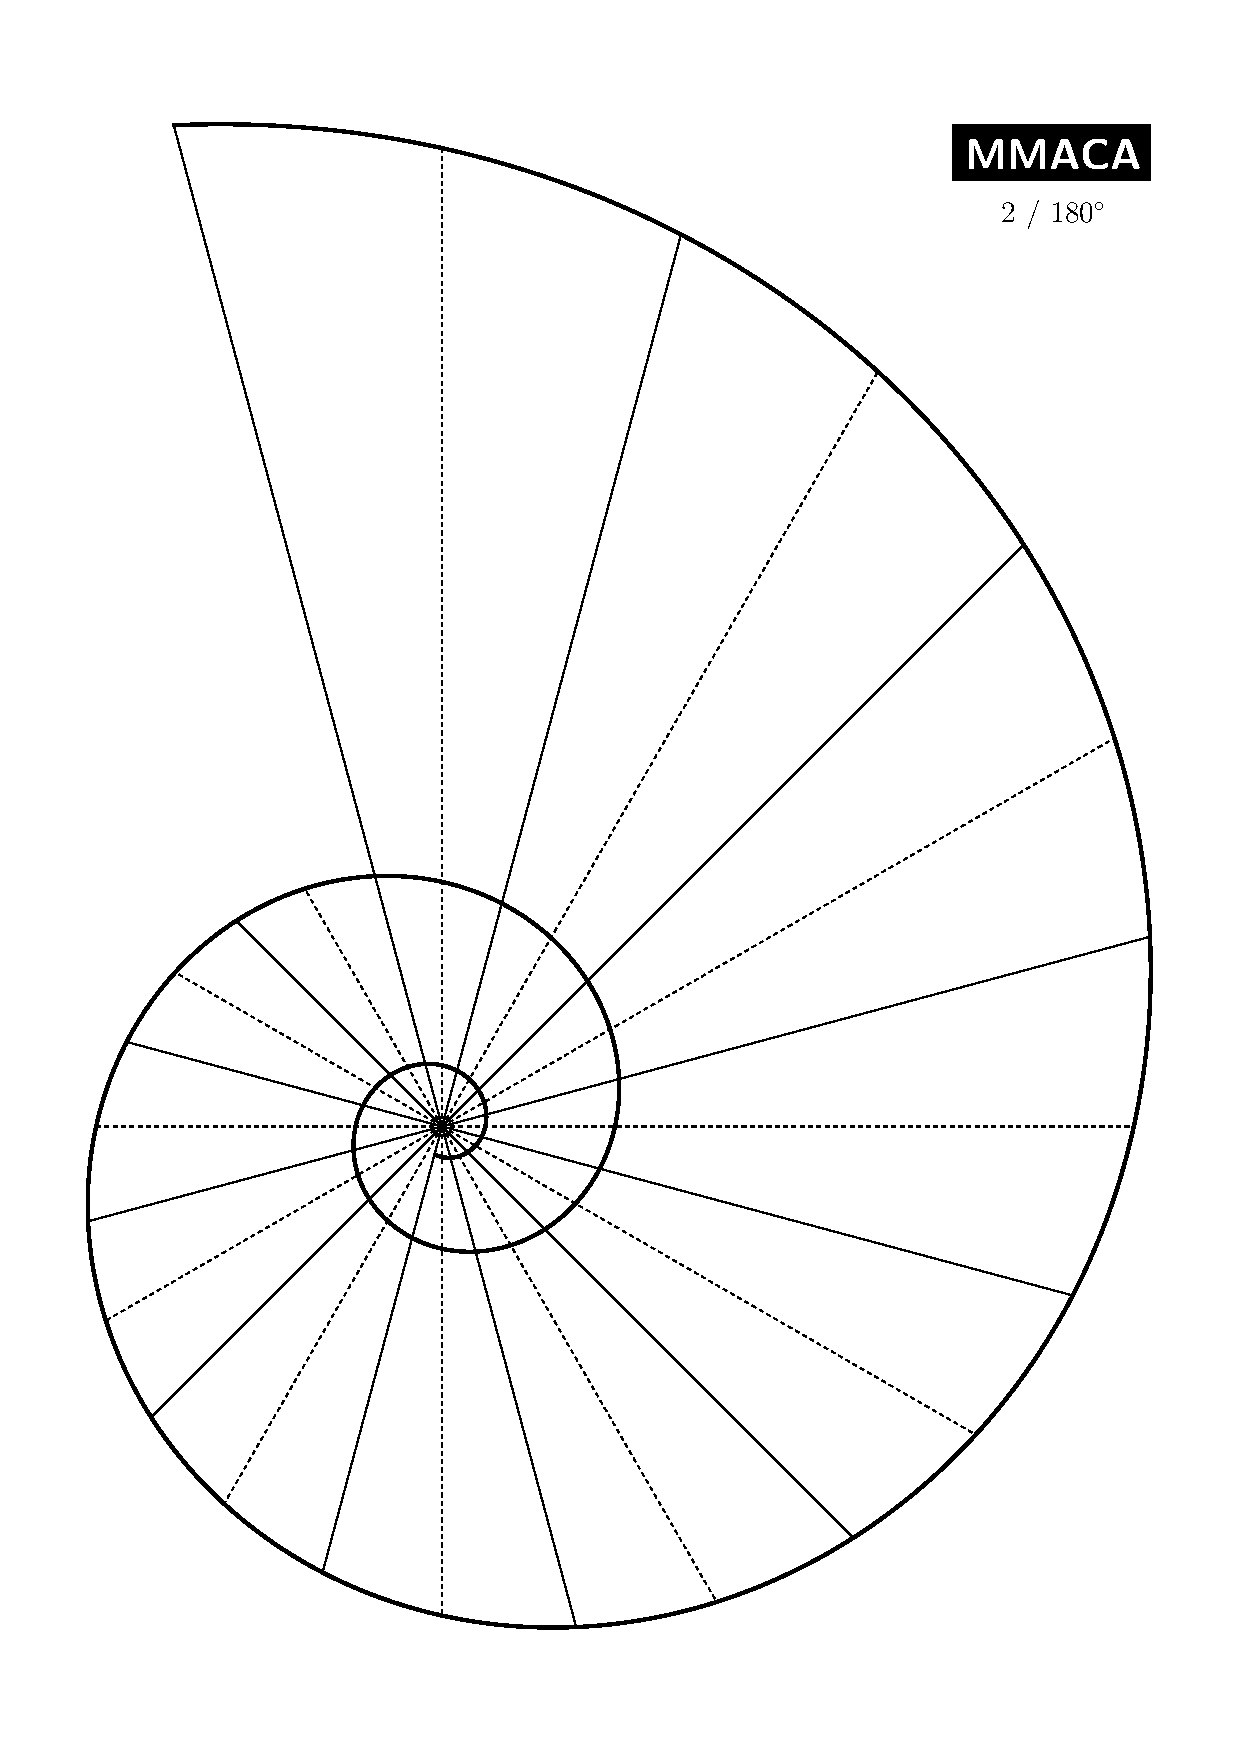
\includepdf{./pictures/Spiral_2_180}
    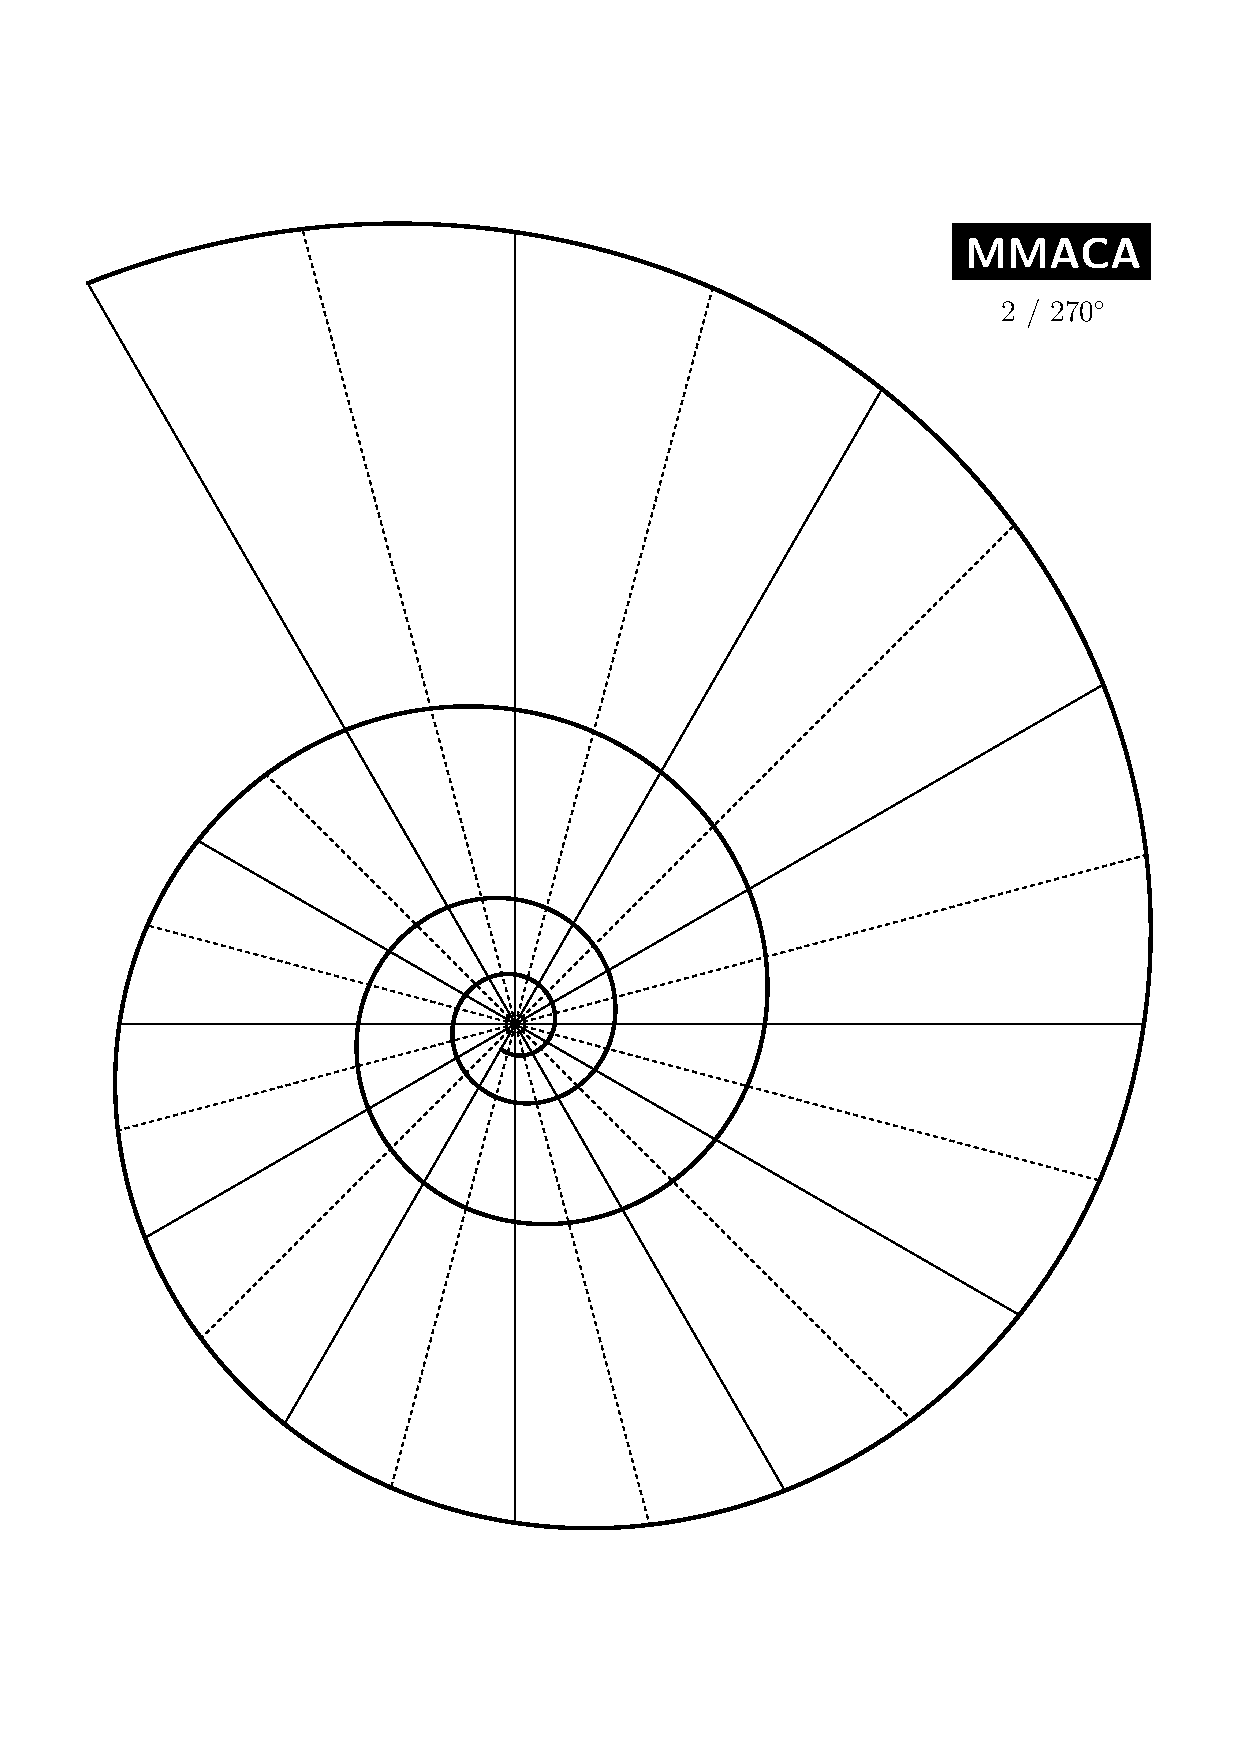
\includepdf{./pictures/Spiral_2_270}
    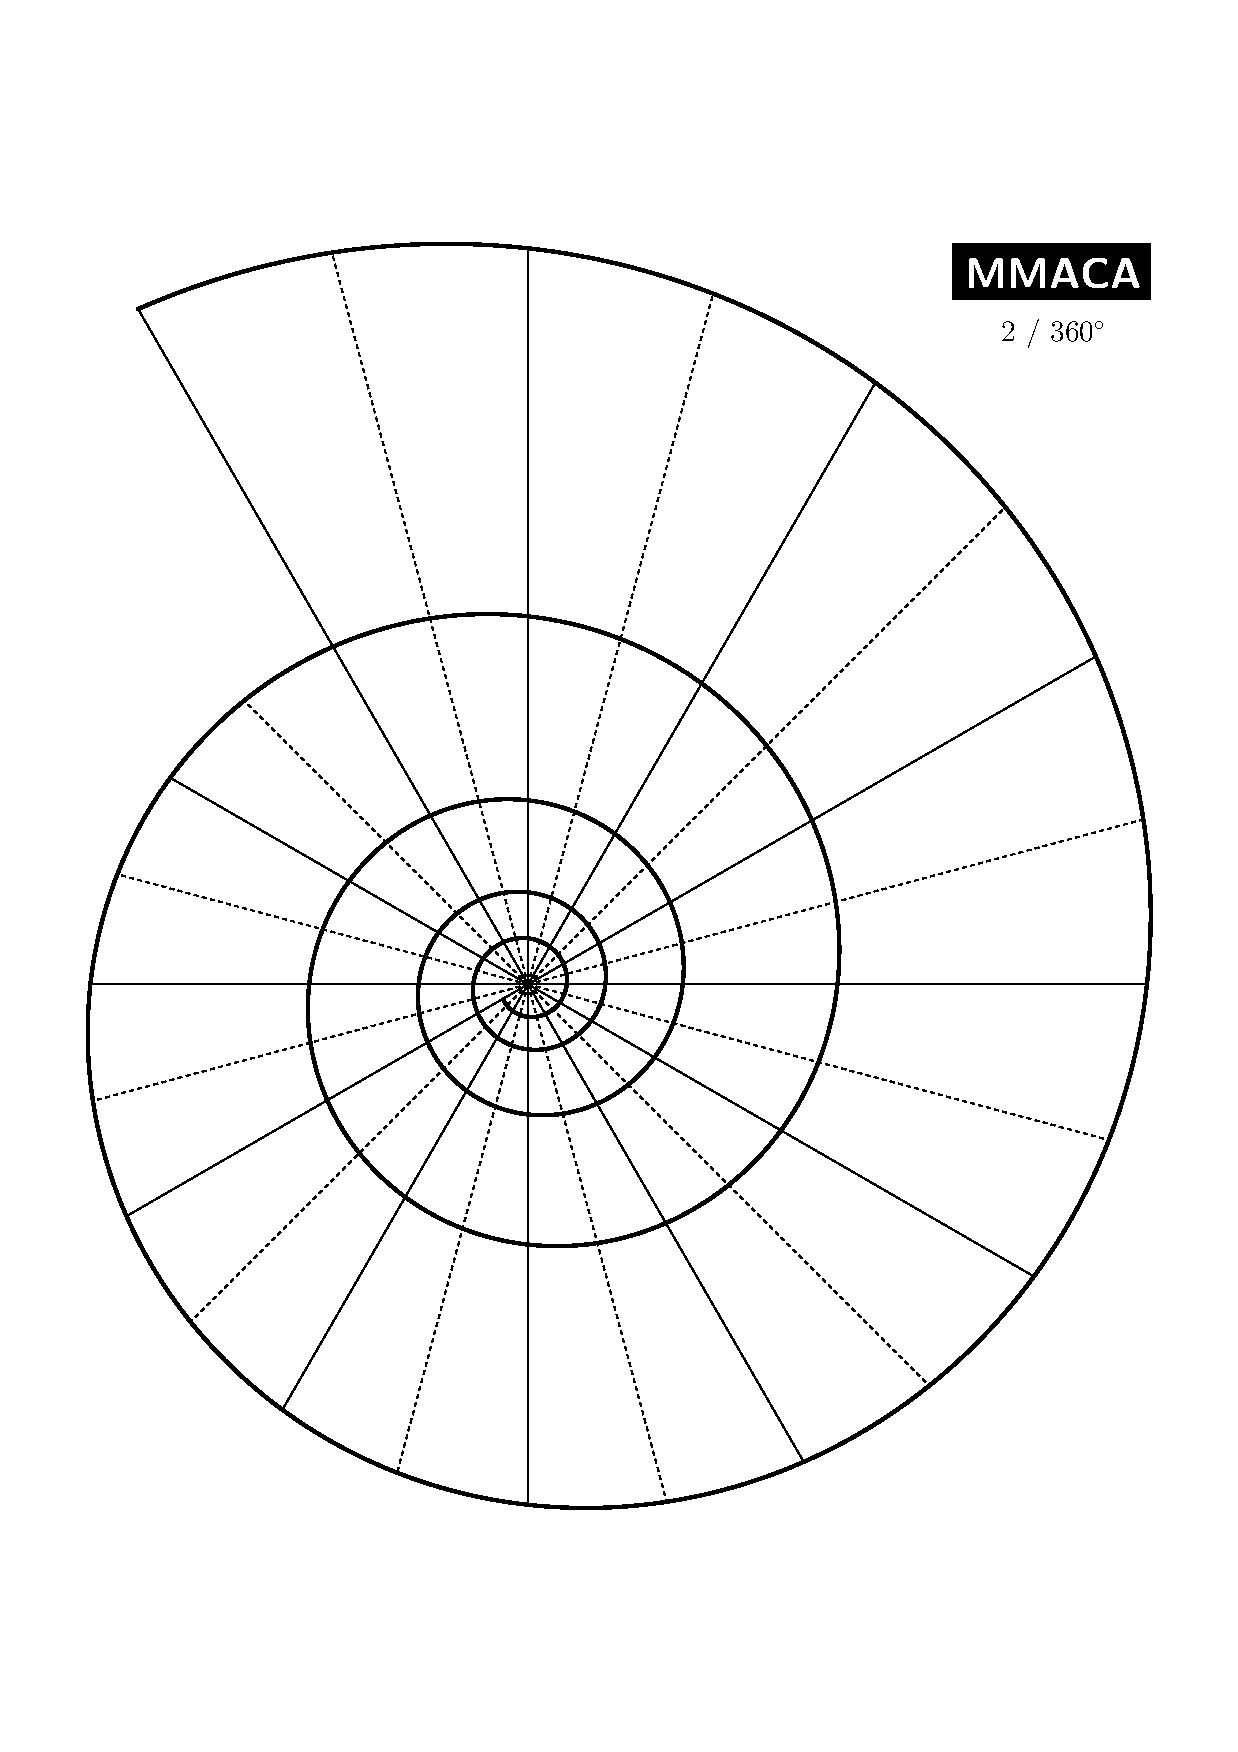
\includepdf{./pictures/Spiral_2_360}
    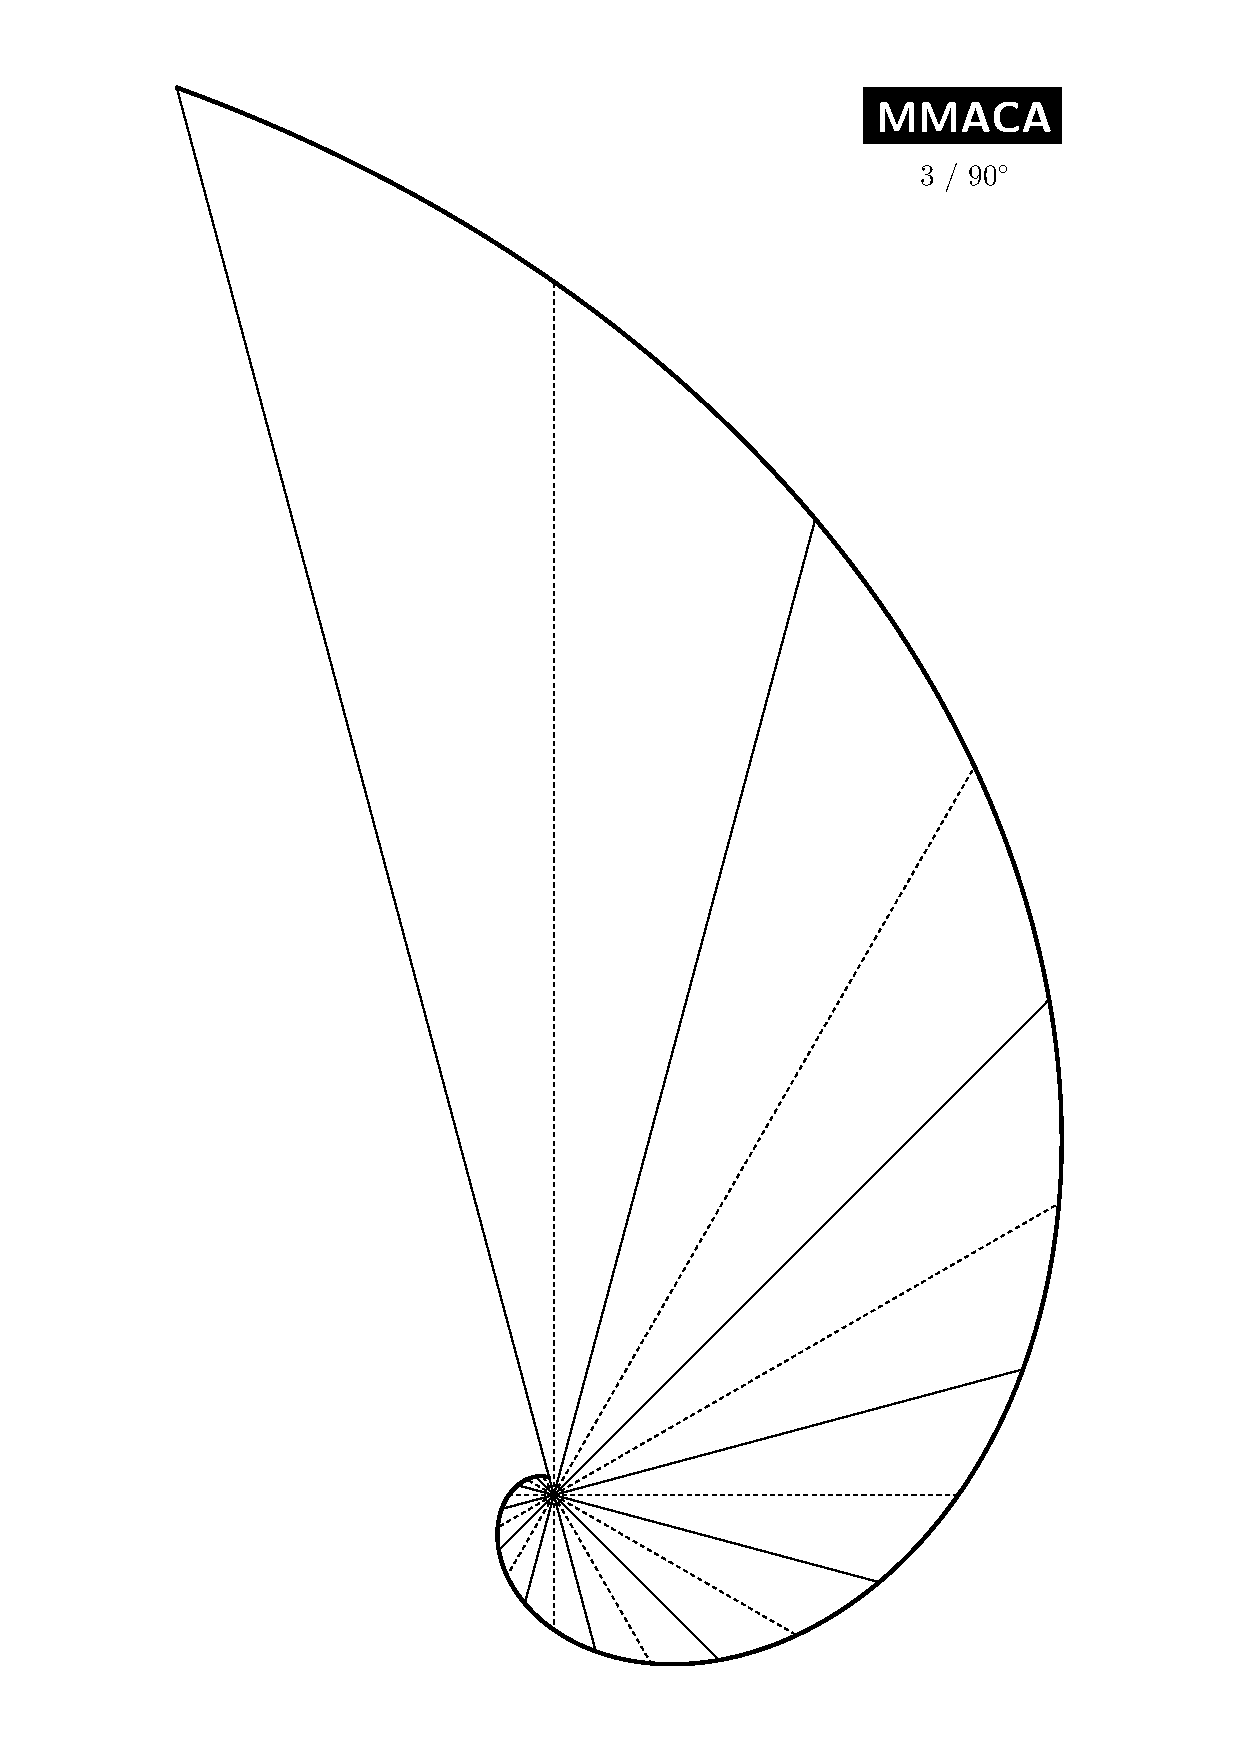
\includepdf{./pictures/Spiral_3_090}
    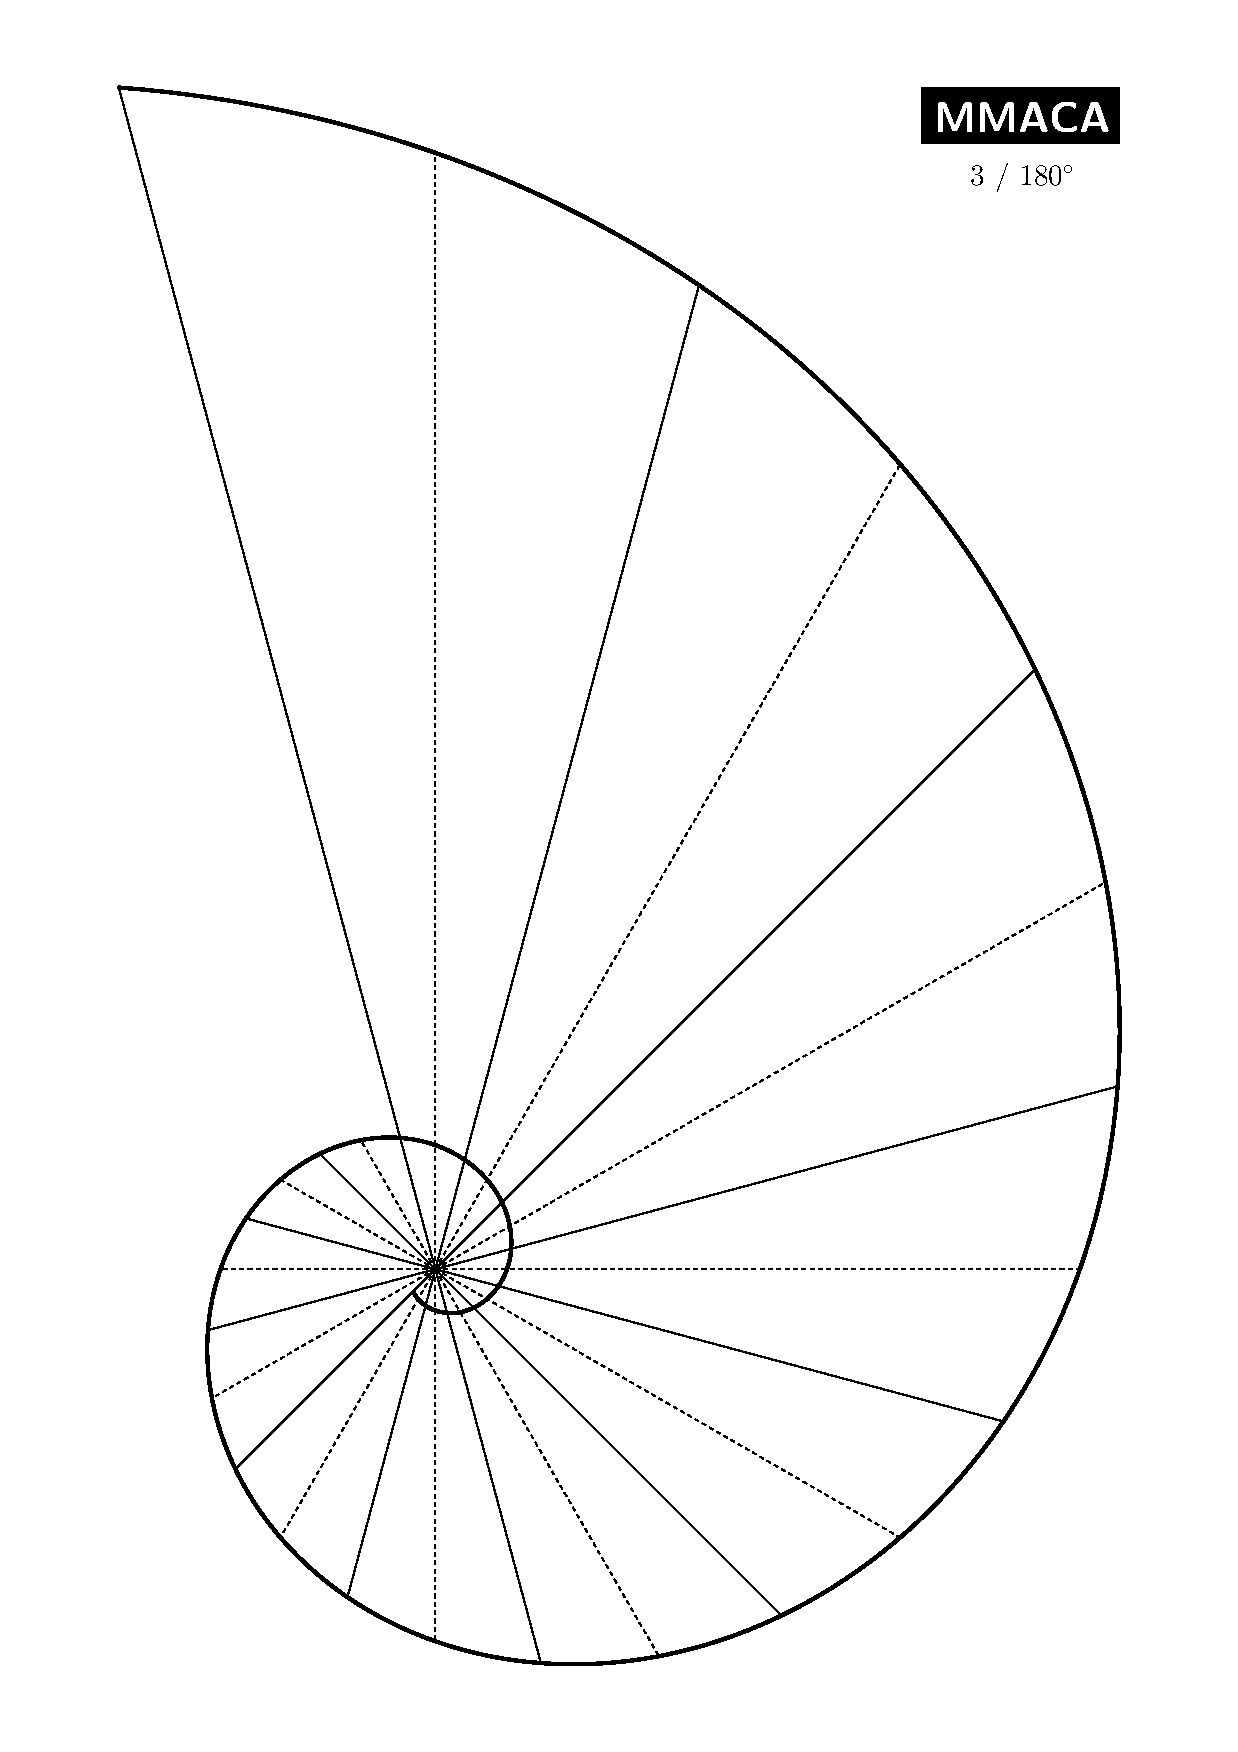
\includepdf{./pictures/Spiral_3_180}
    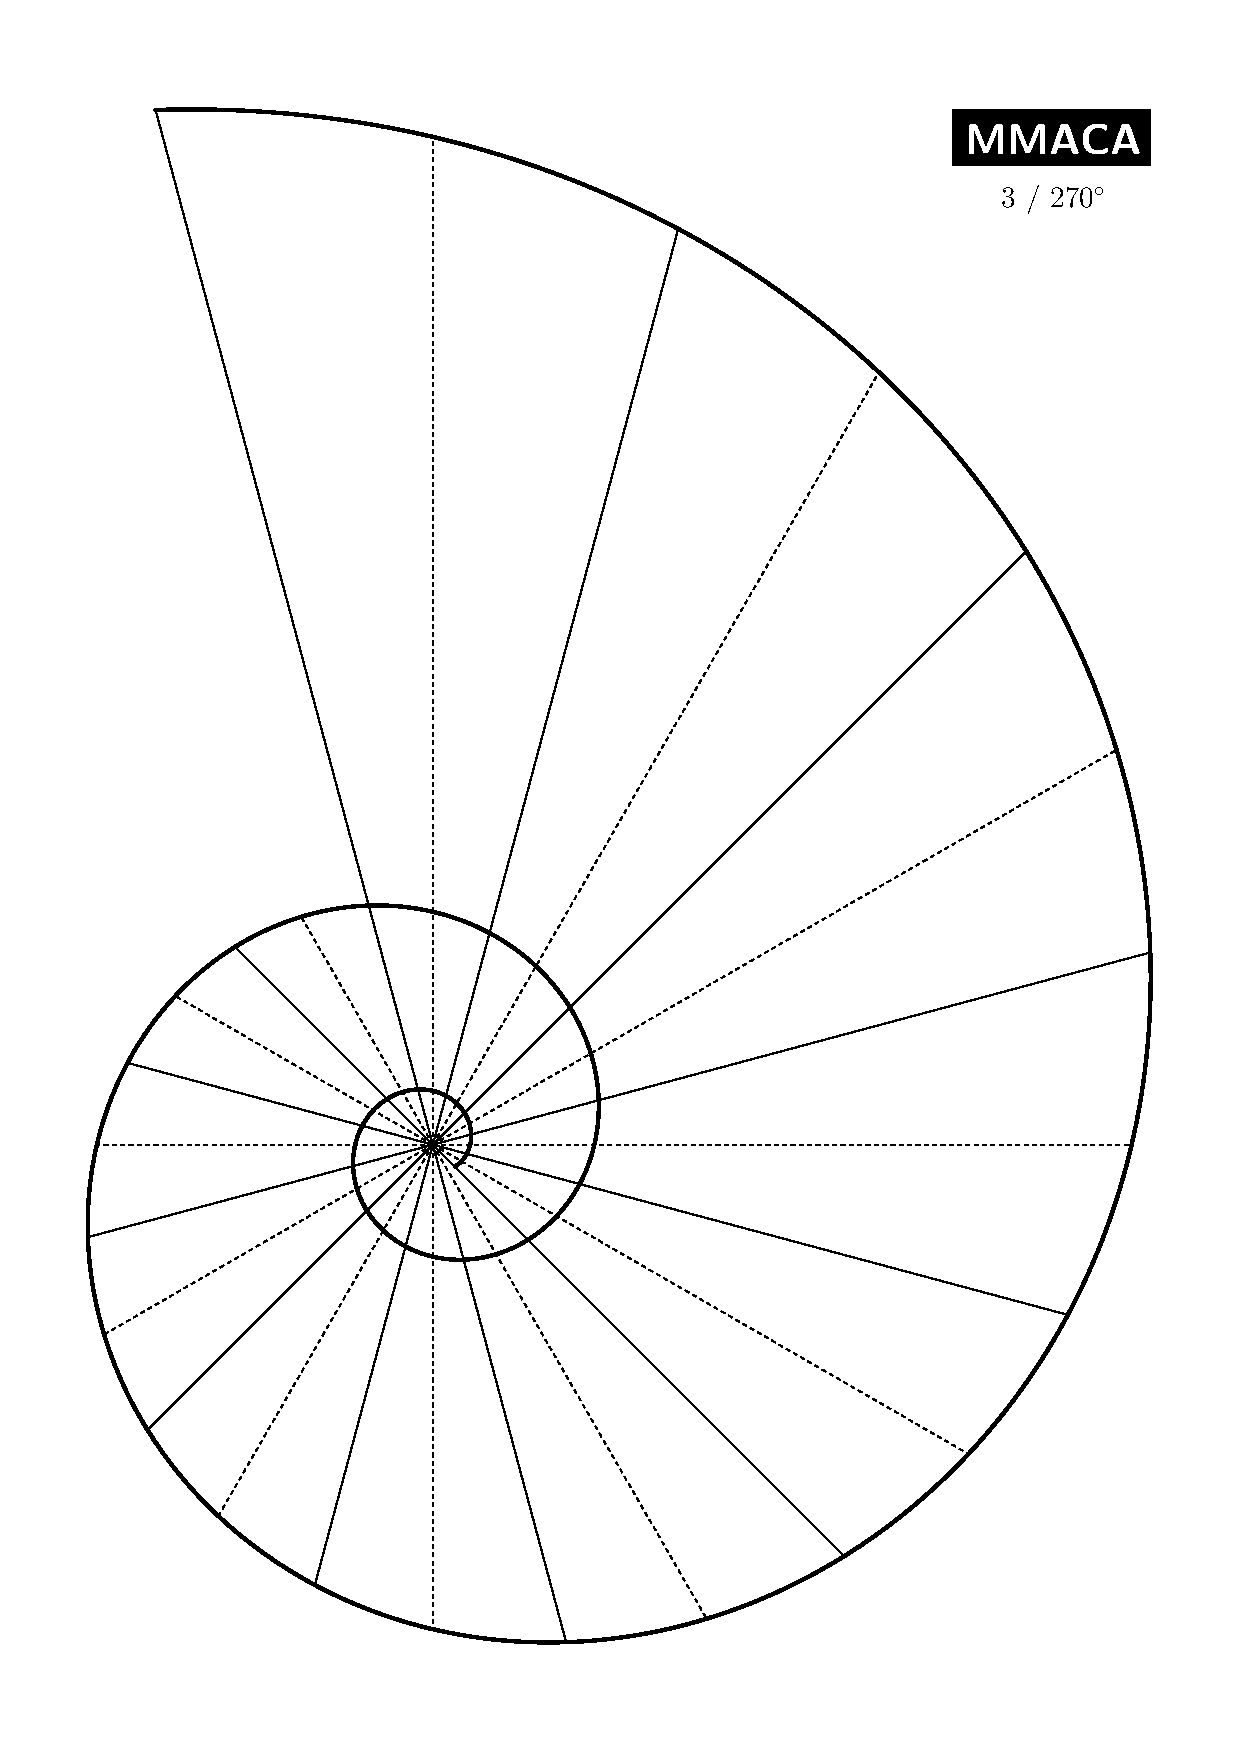
\includepdf{./pictures/Spiral_3_270}
    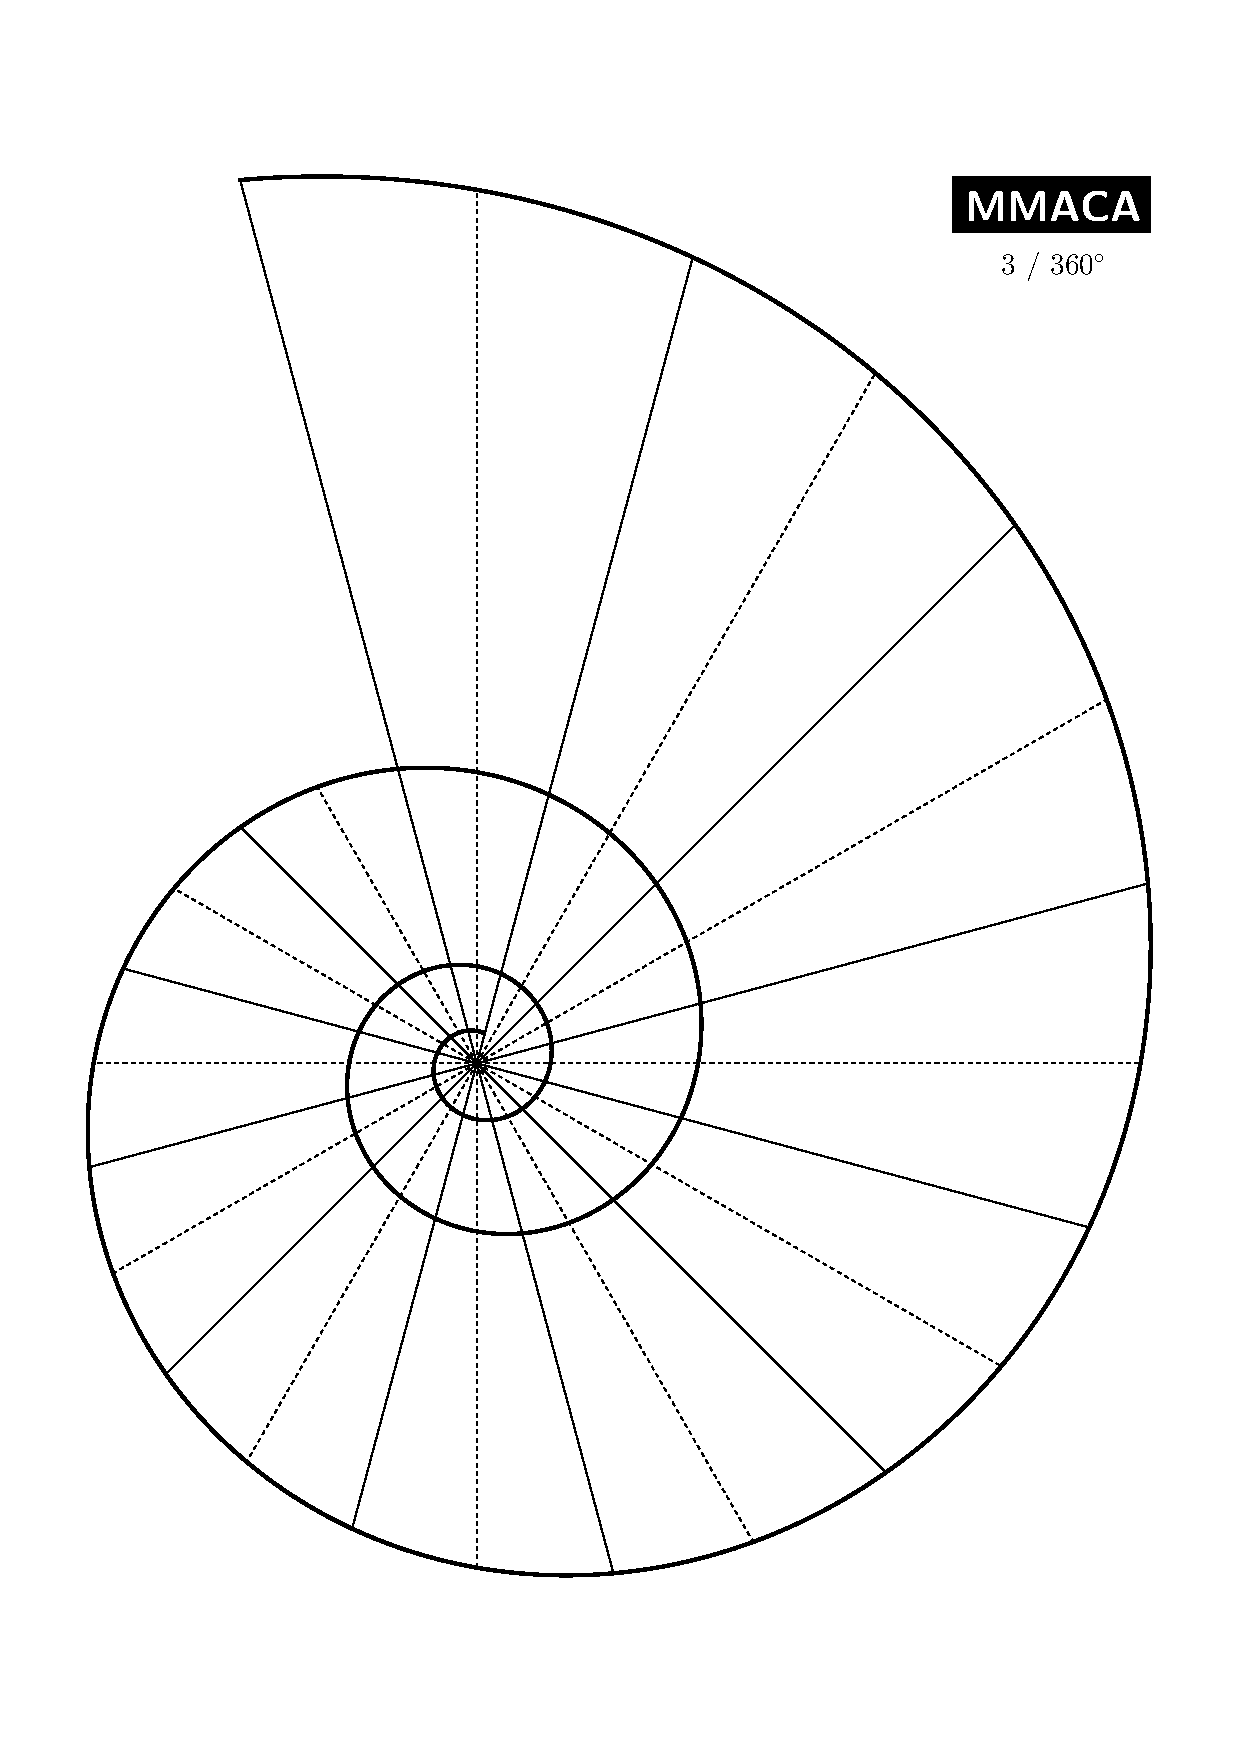
\includepdf{./pictures/Spiral_3_360}
    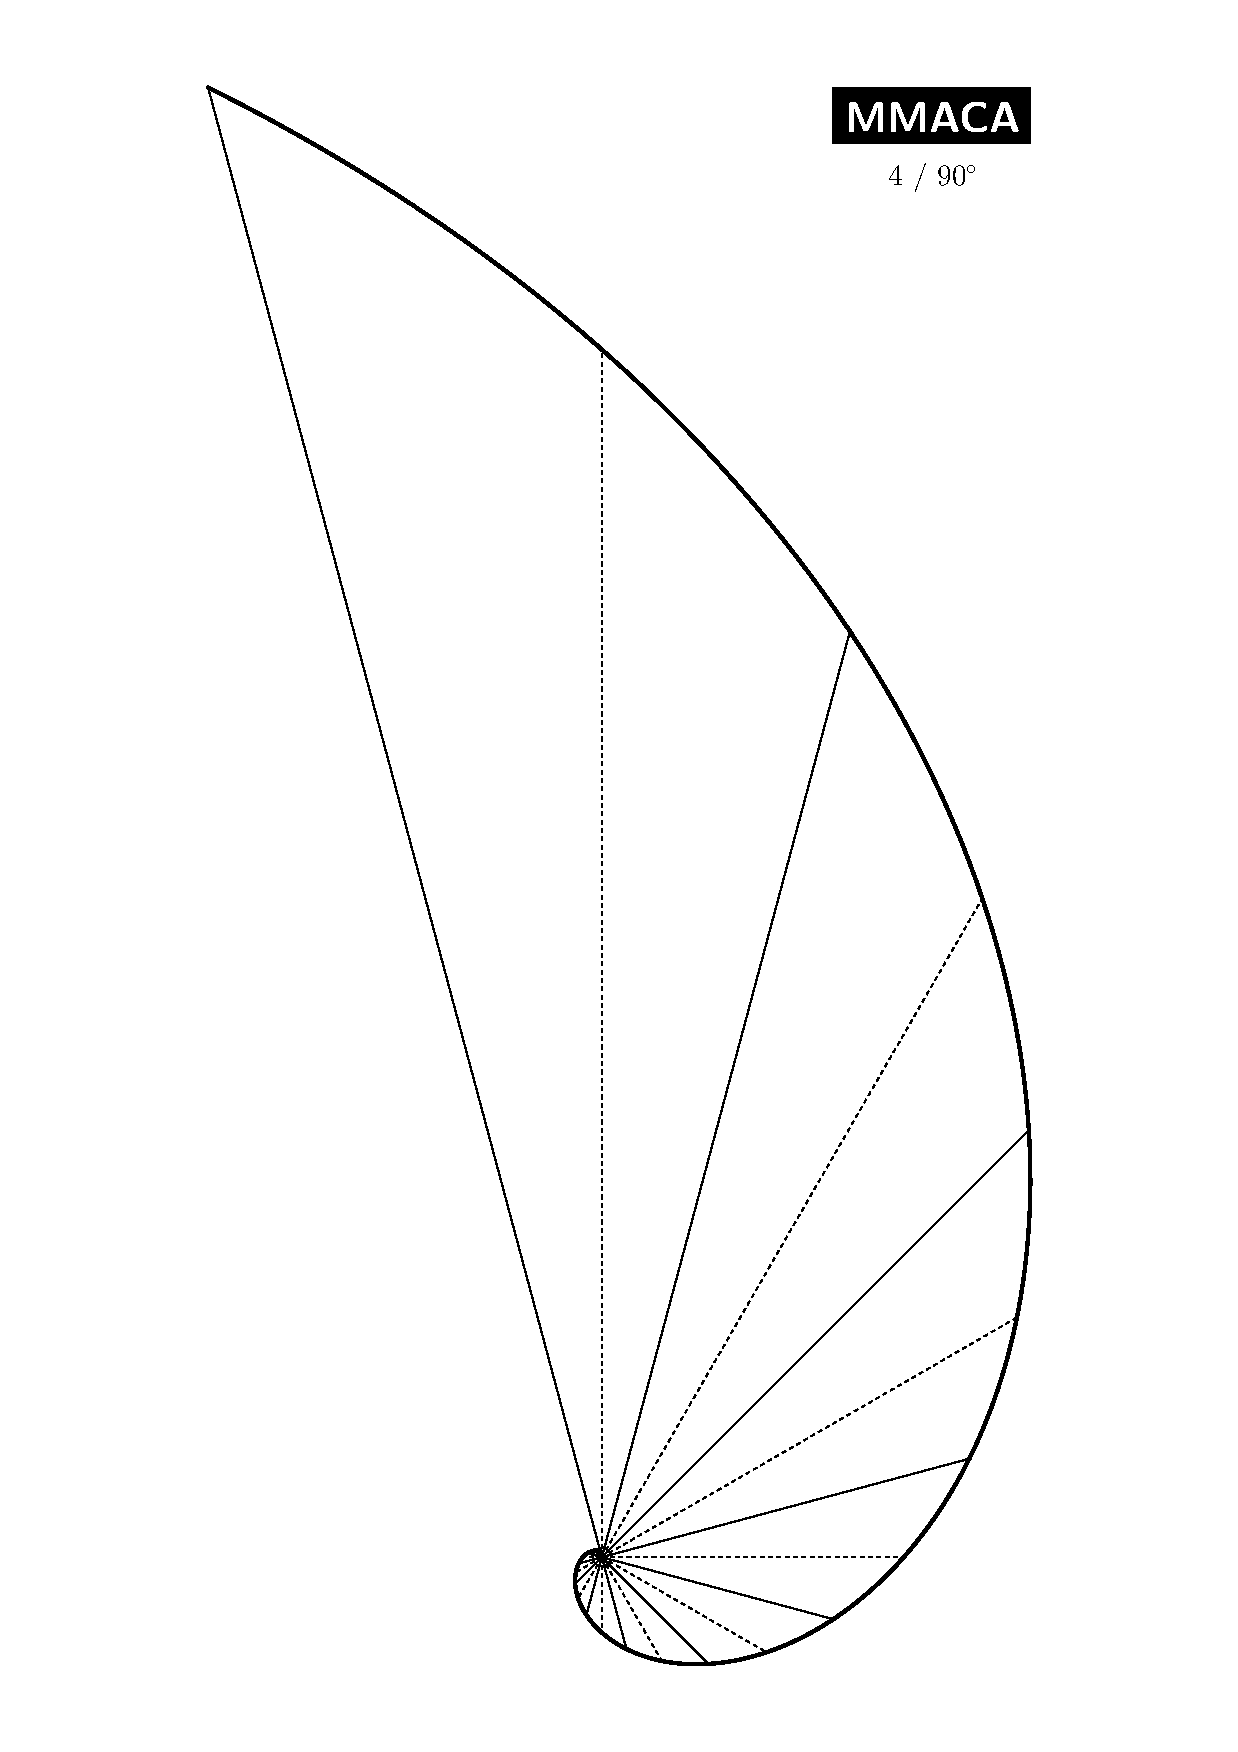
\includepdf{./pictures/Spiral_4_090}
    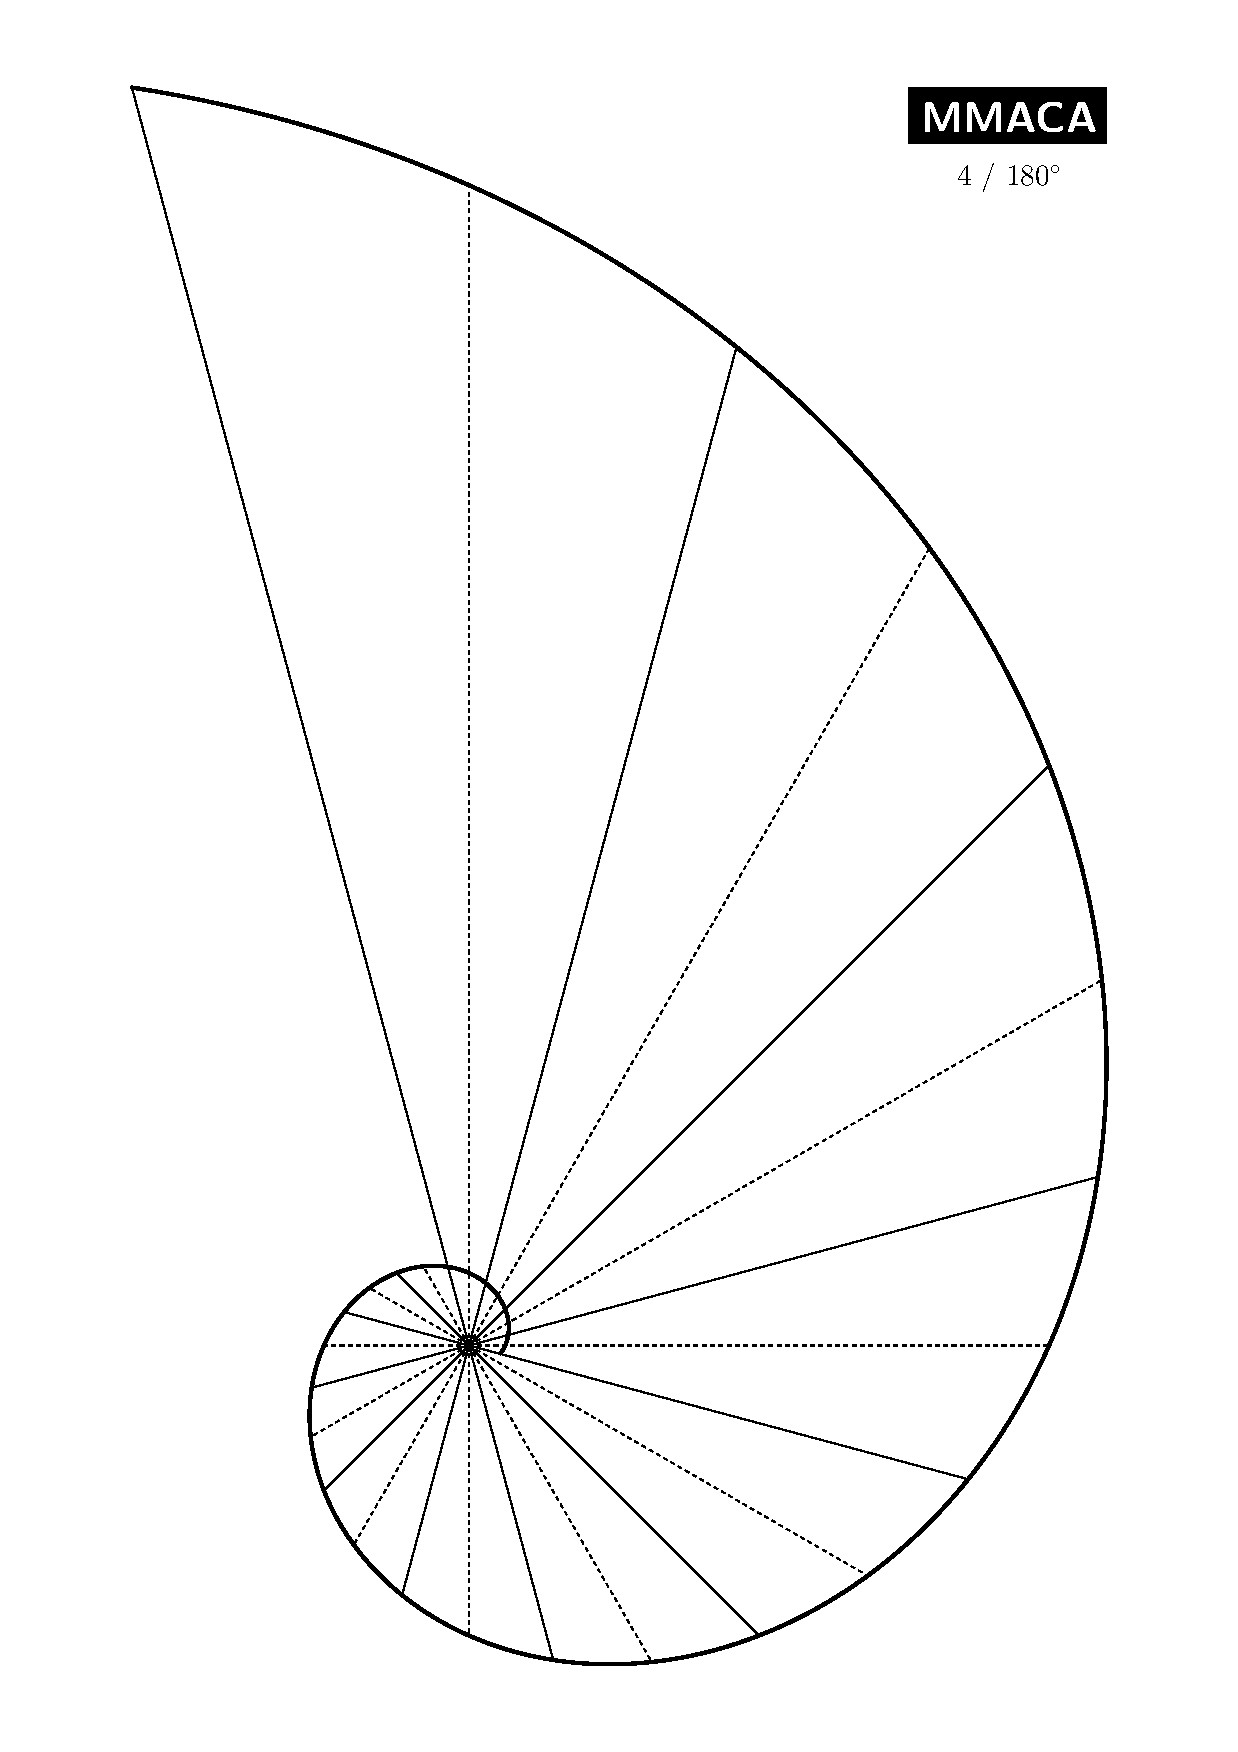
\includepdf{./pictures/Spiral_4_180}
    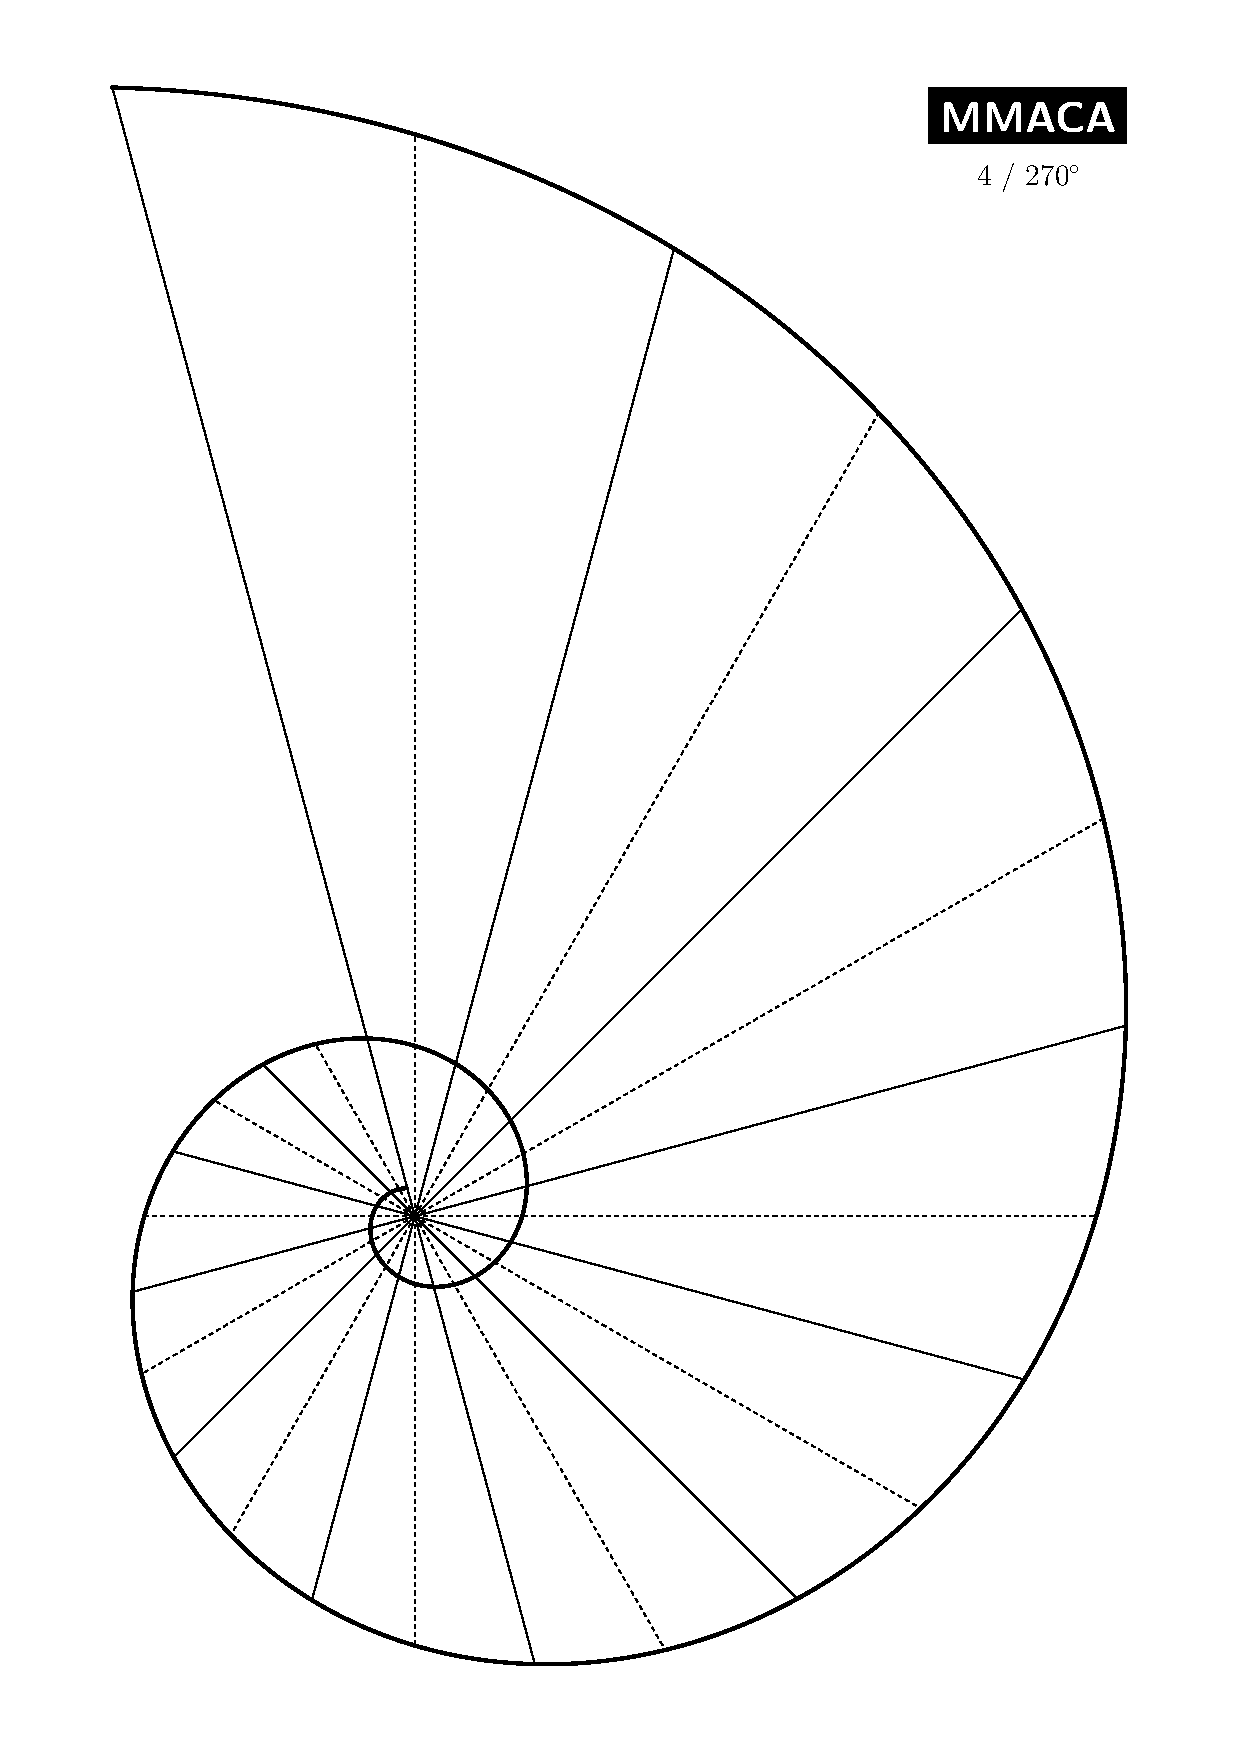
\includepdf{./pictures/Spiral_4_270}
    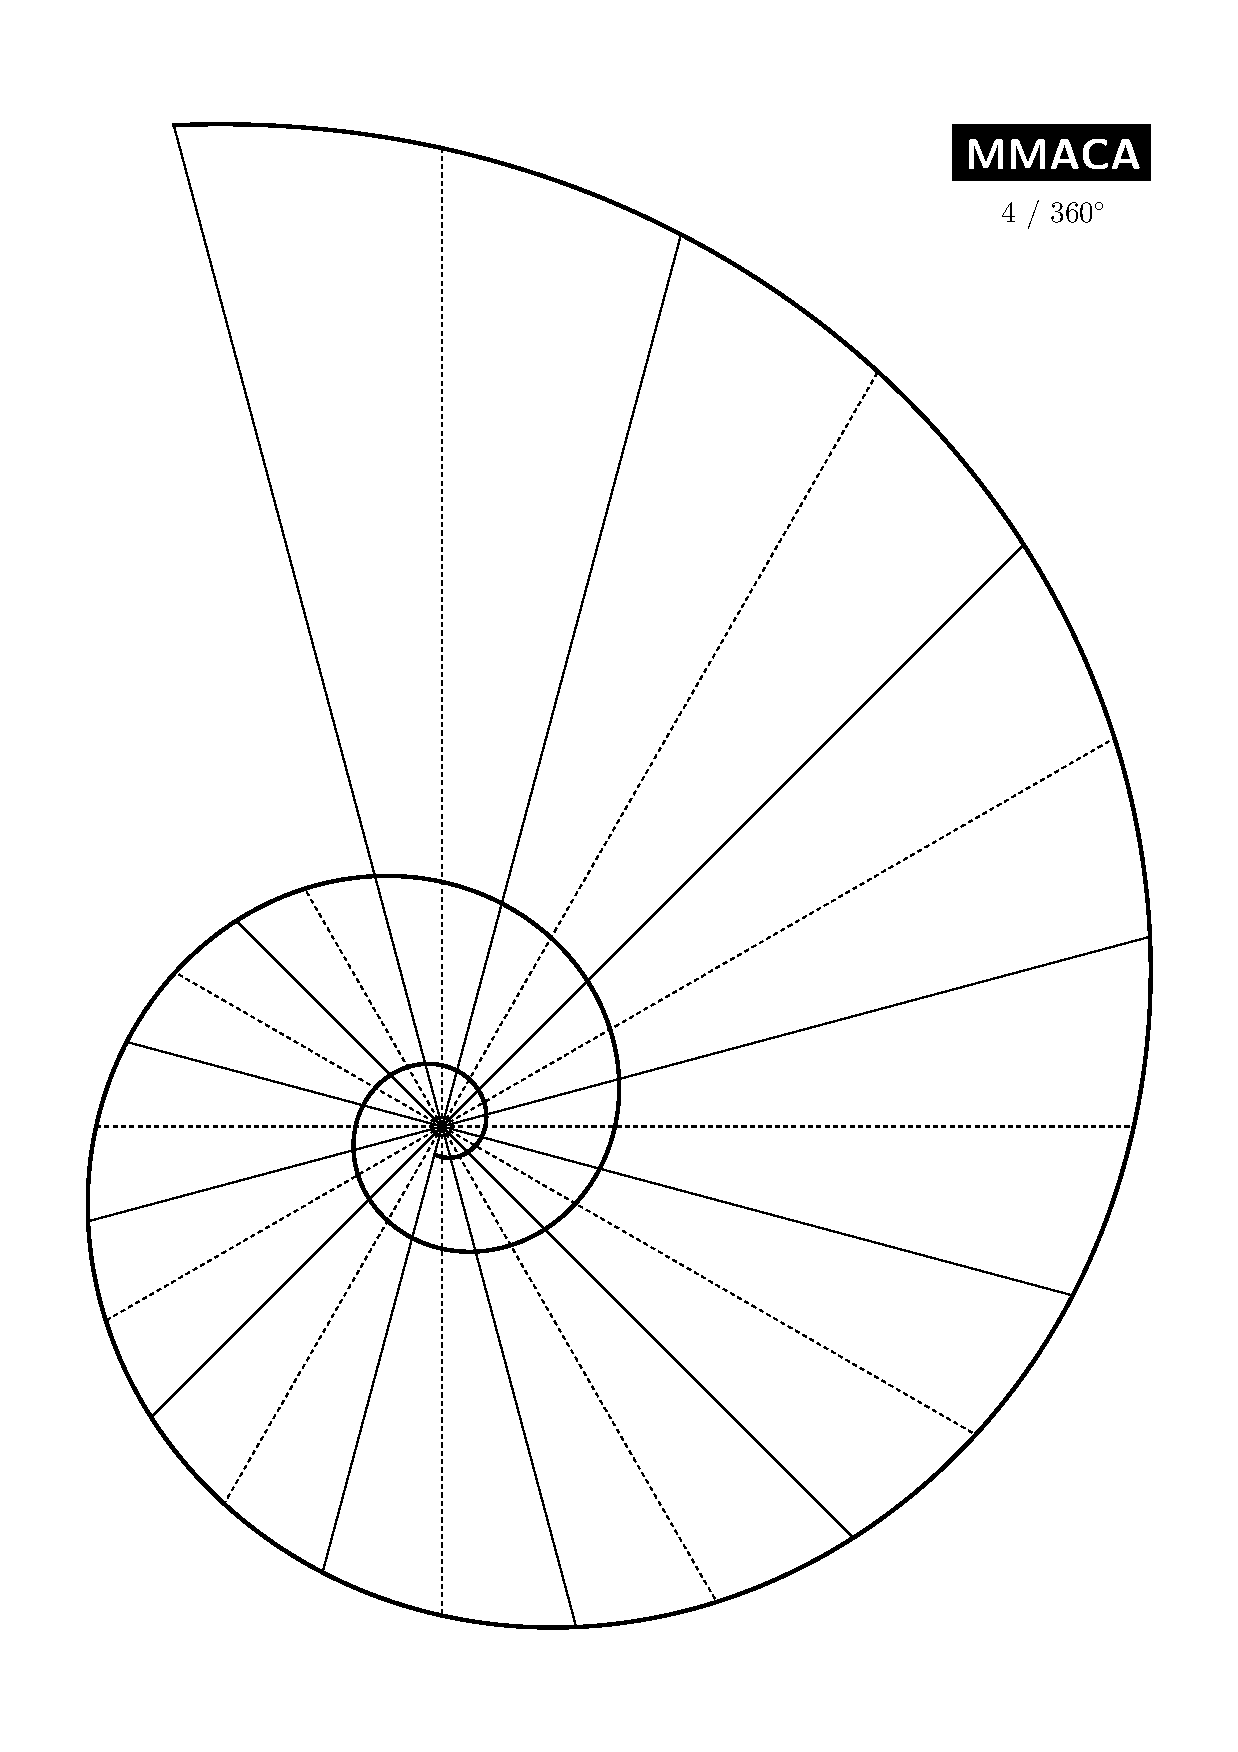
\includepdf{./pictures/Spiral_4_360}
    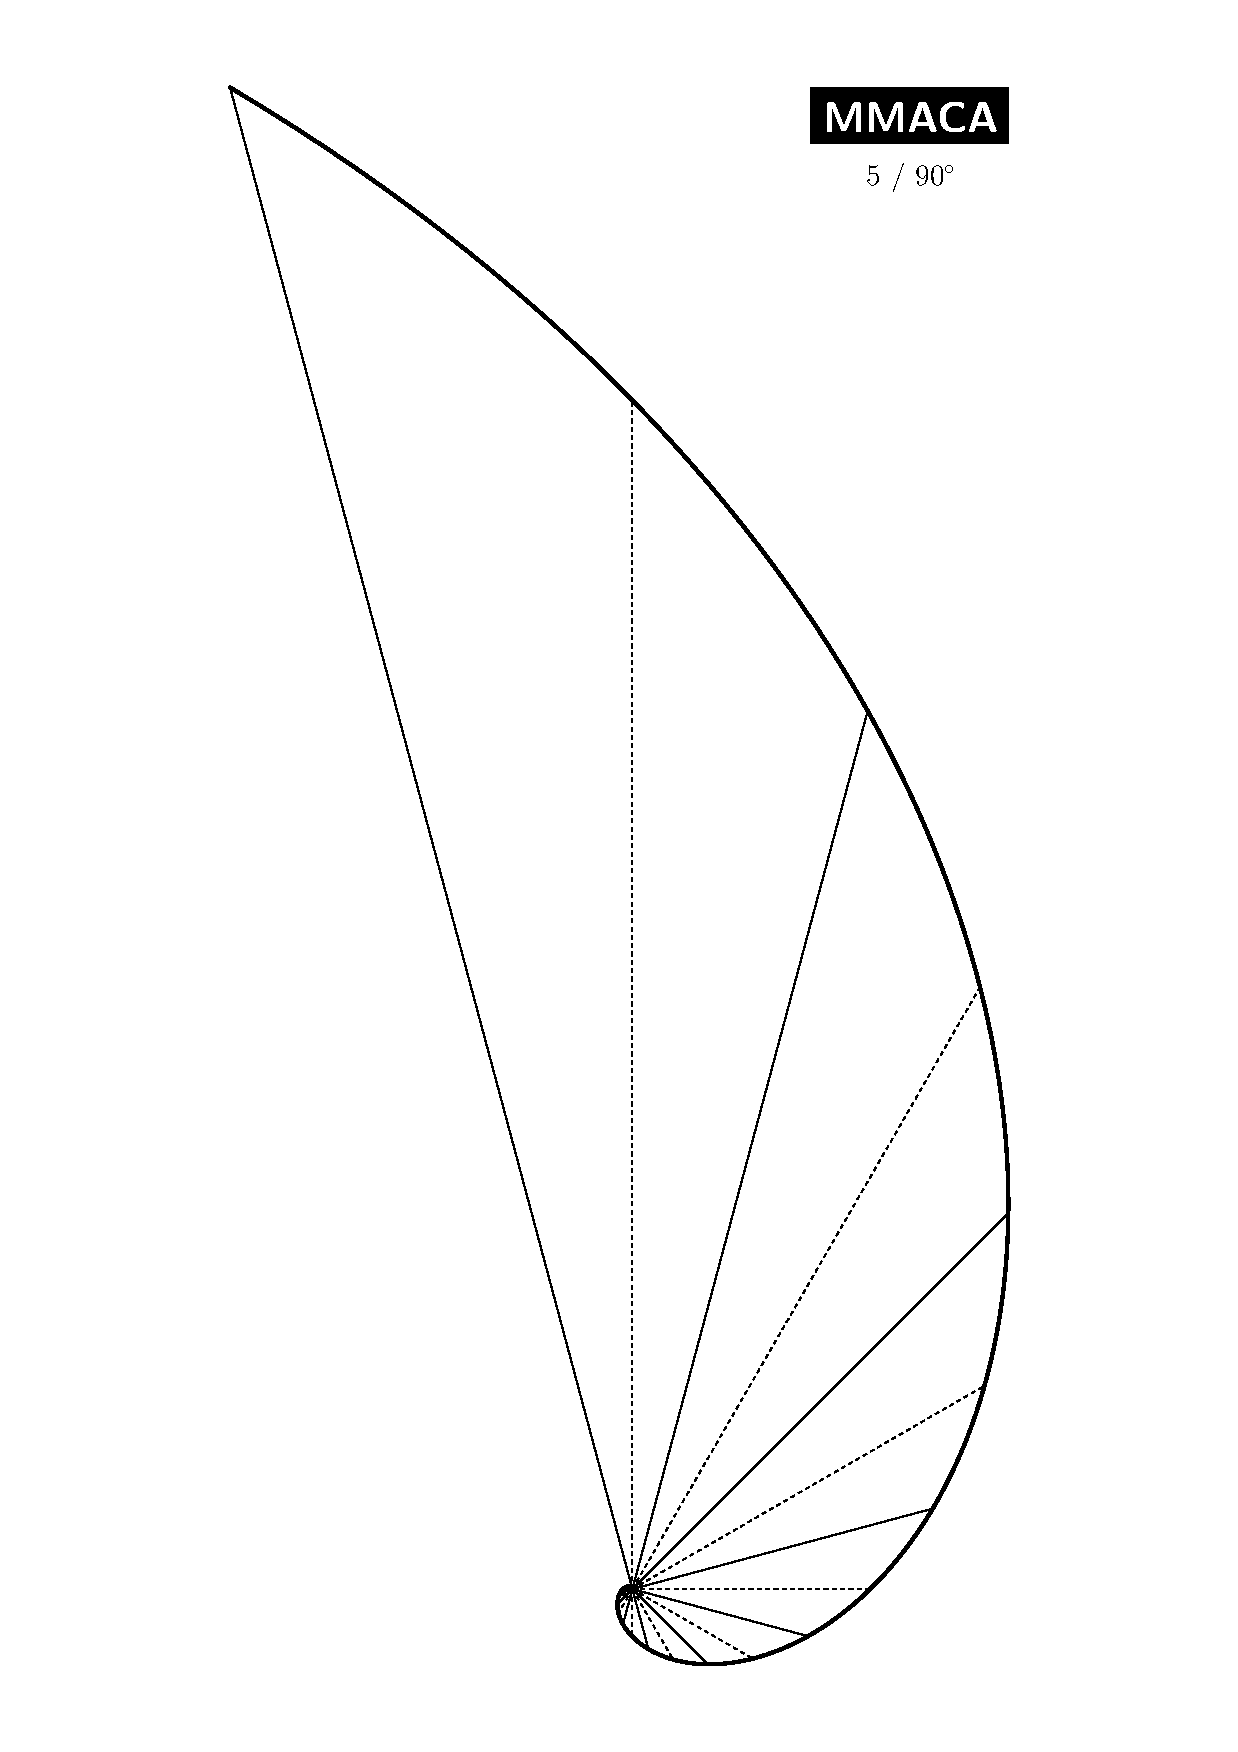
\includepdf{./pictures/Spiral_5_090}
    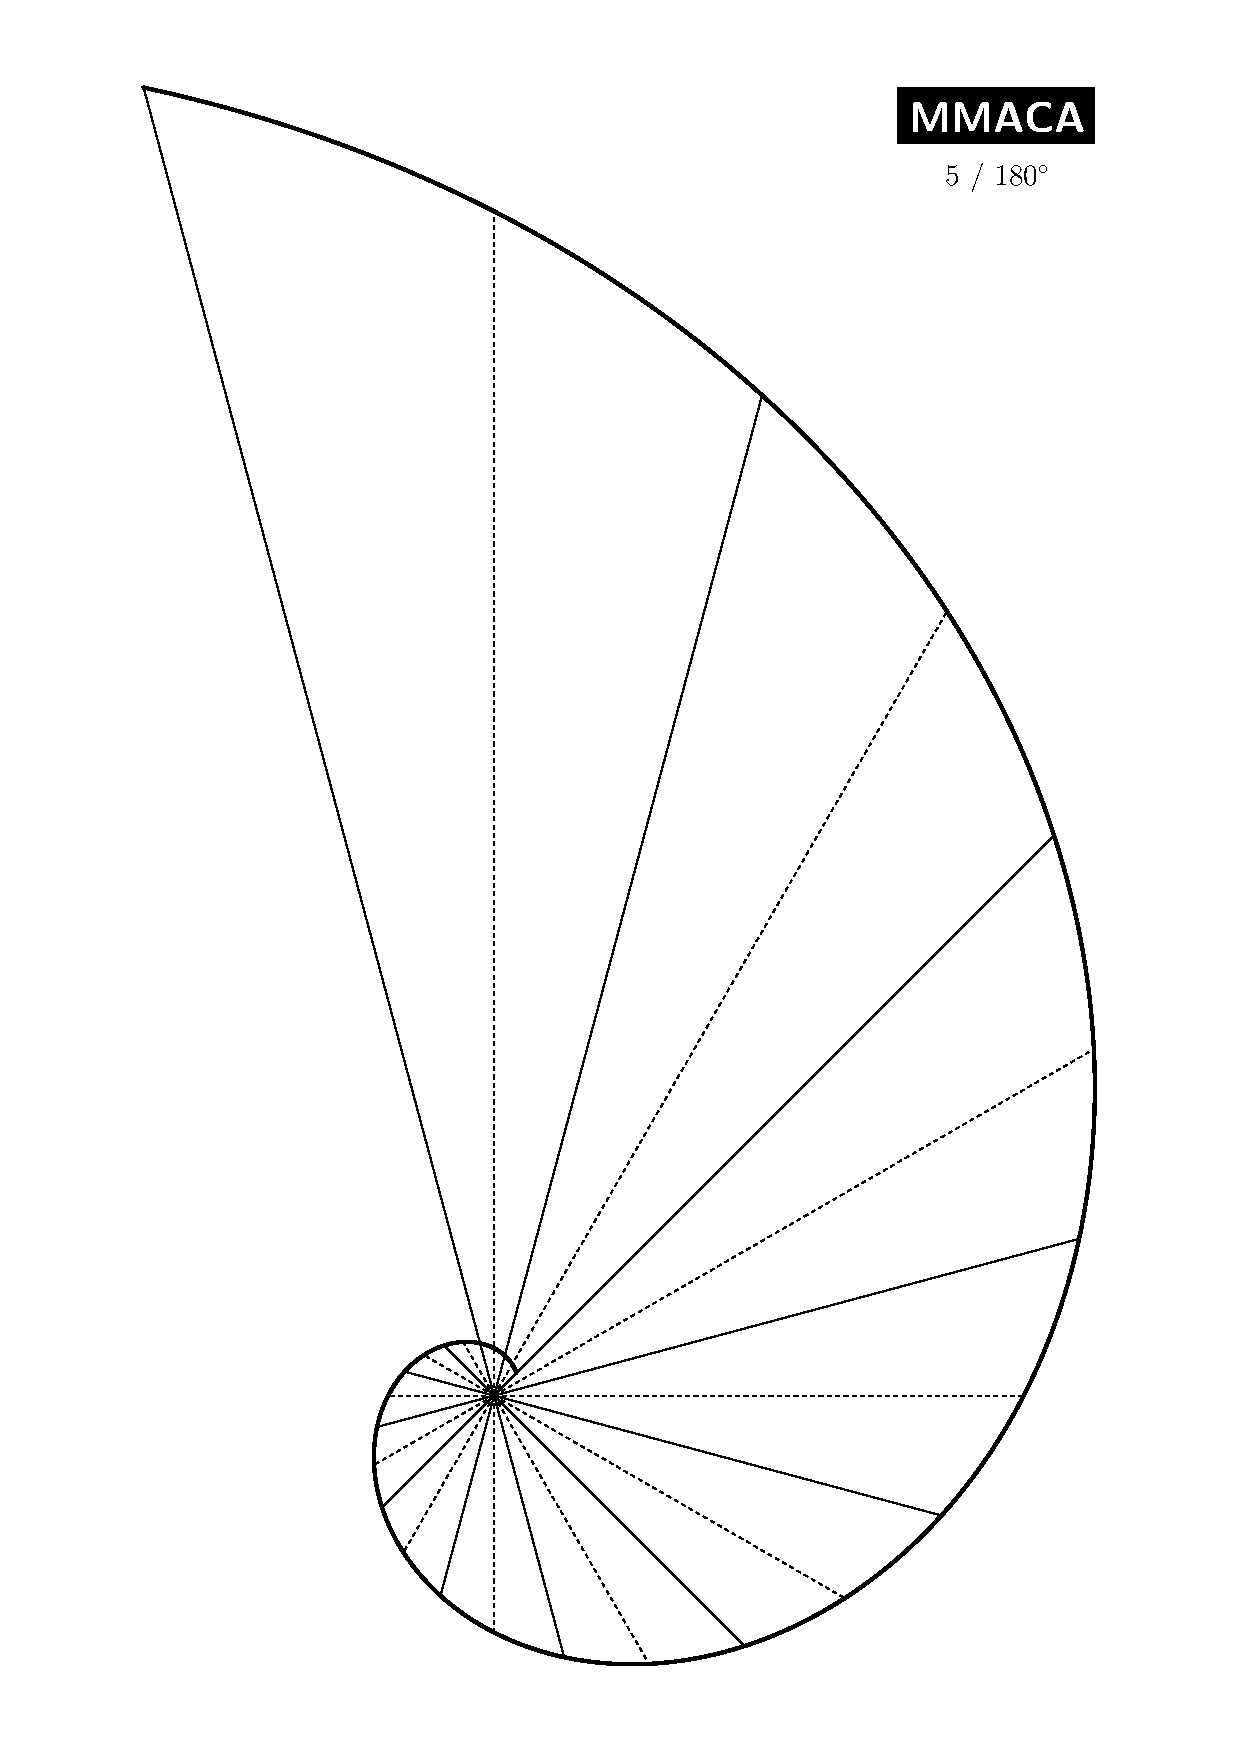
\includepdf{./pictures/Spiral_5_180}
    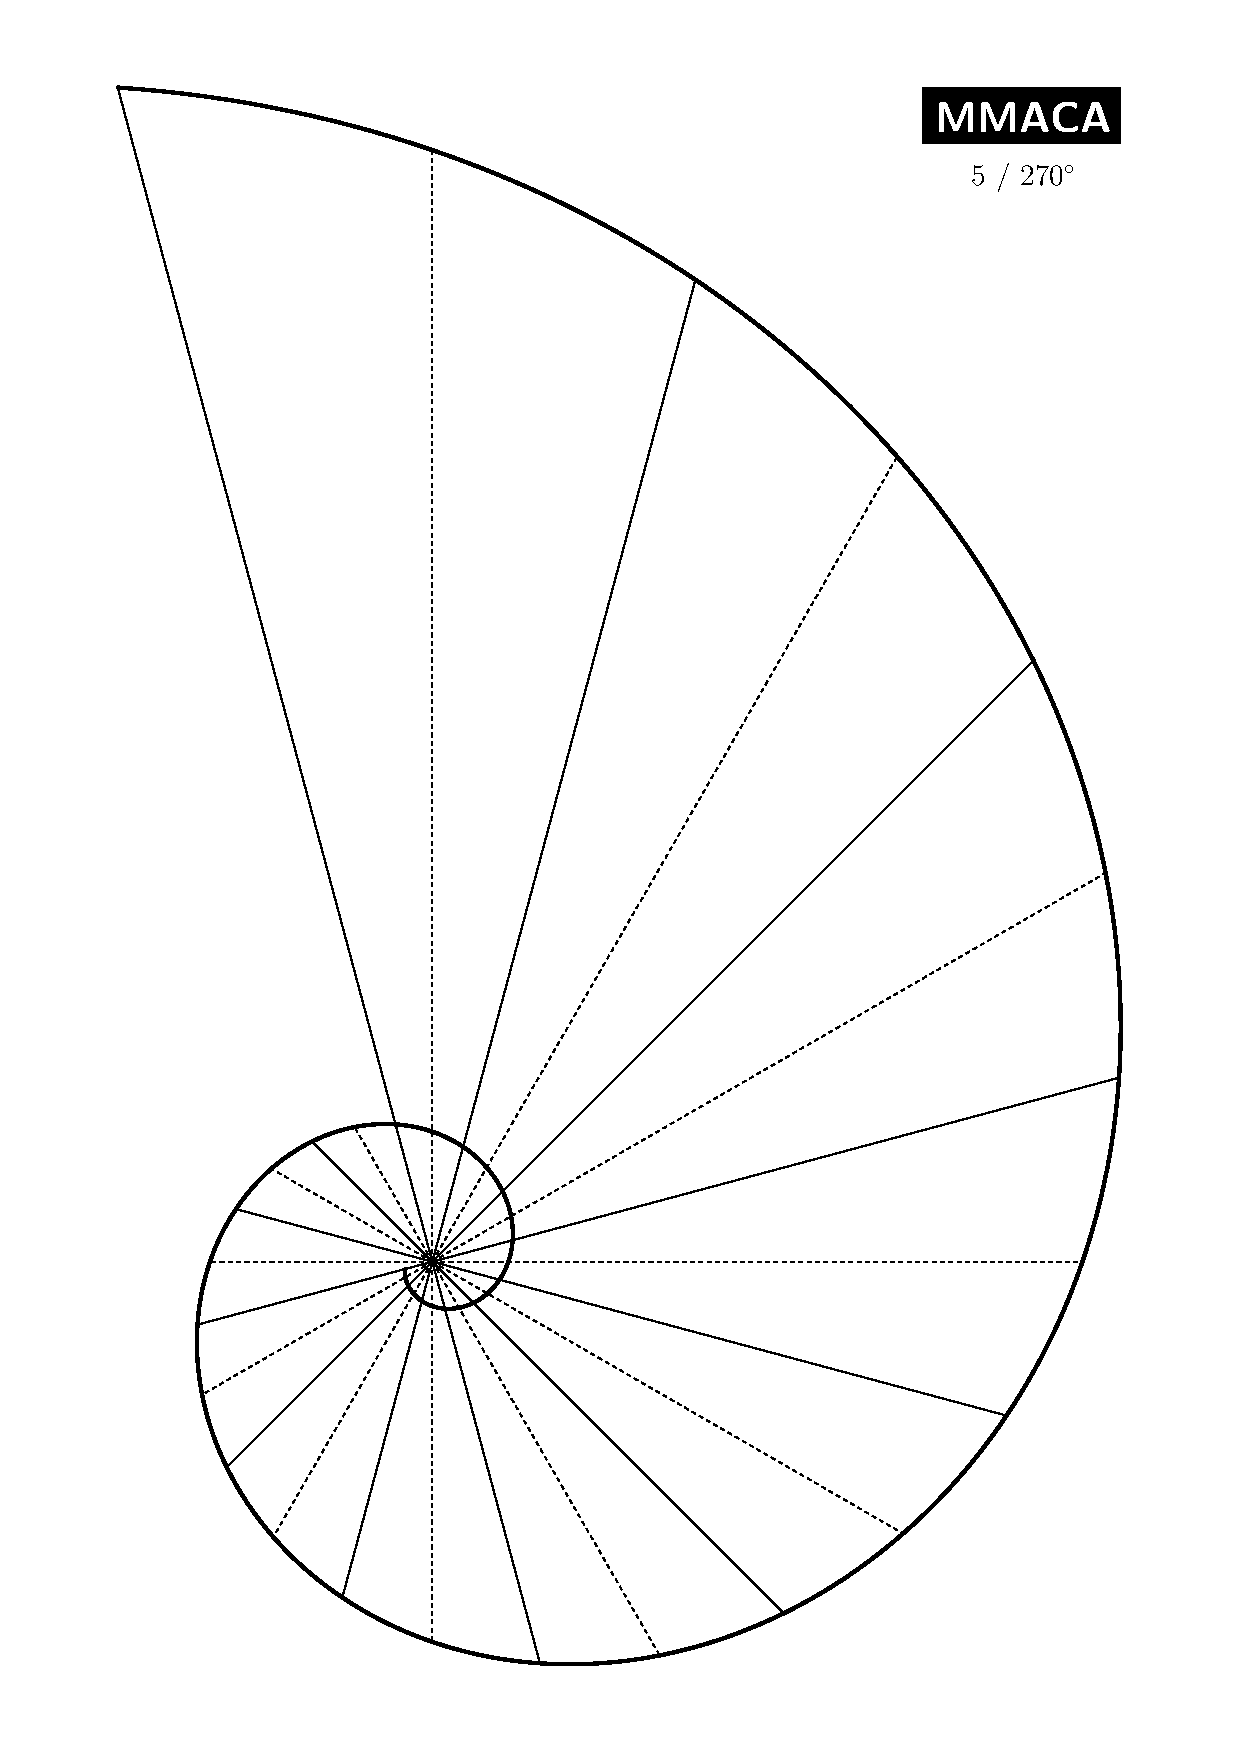
\includepdf{./pictures/Spiral_5_270}
    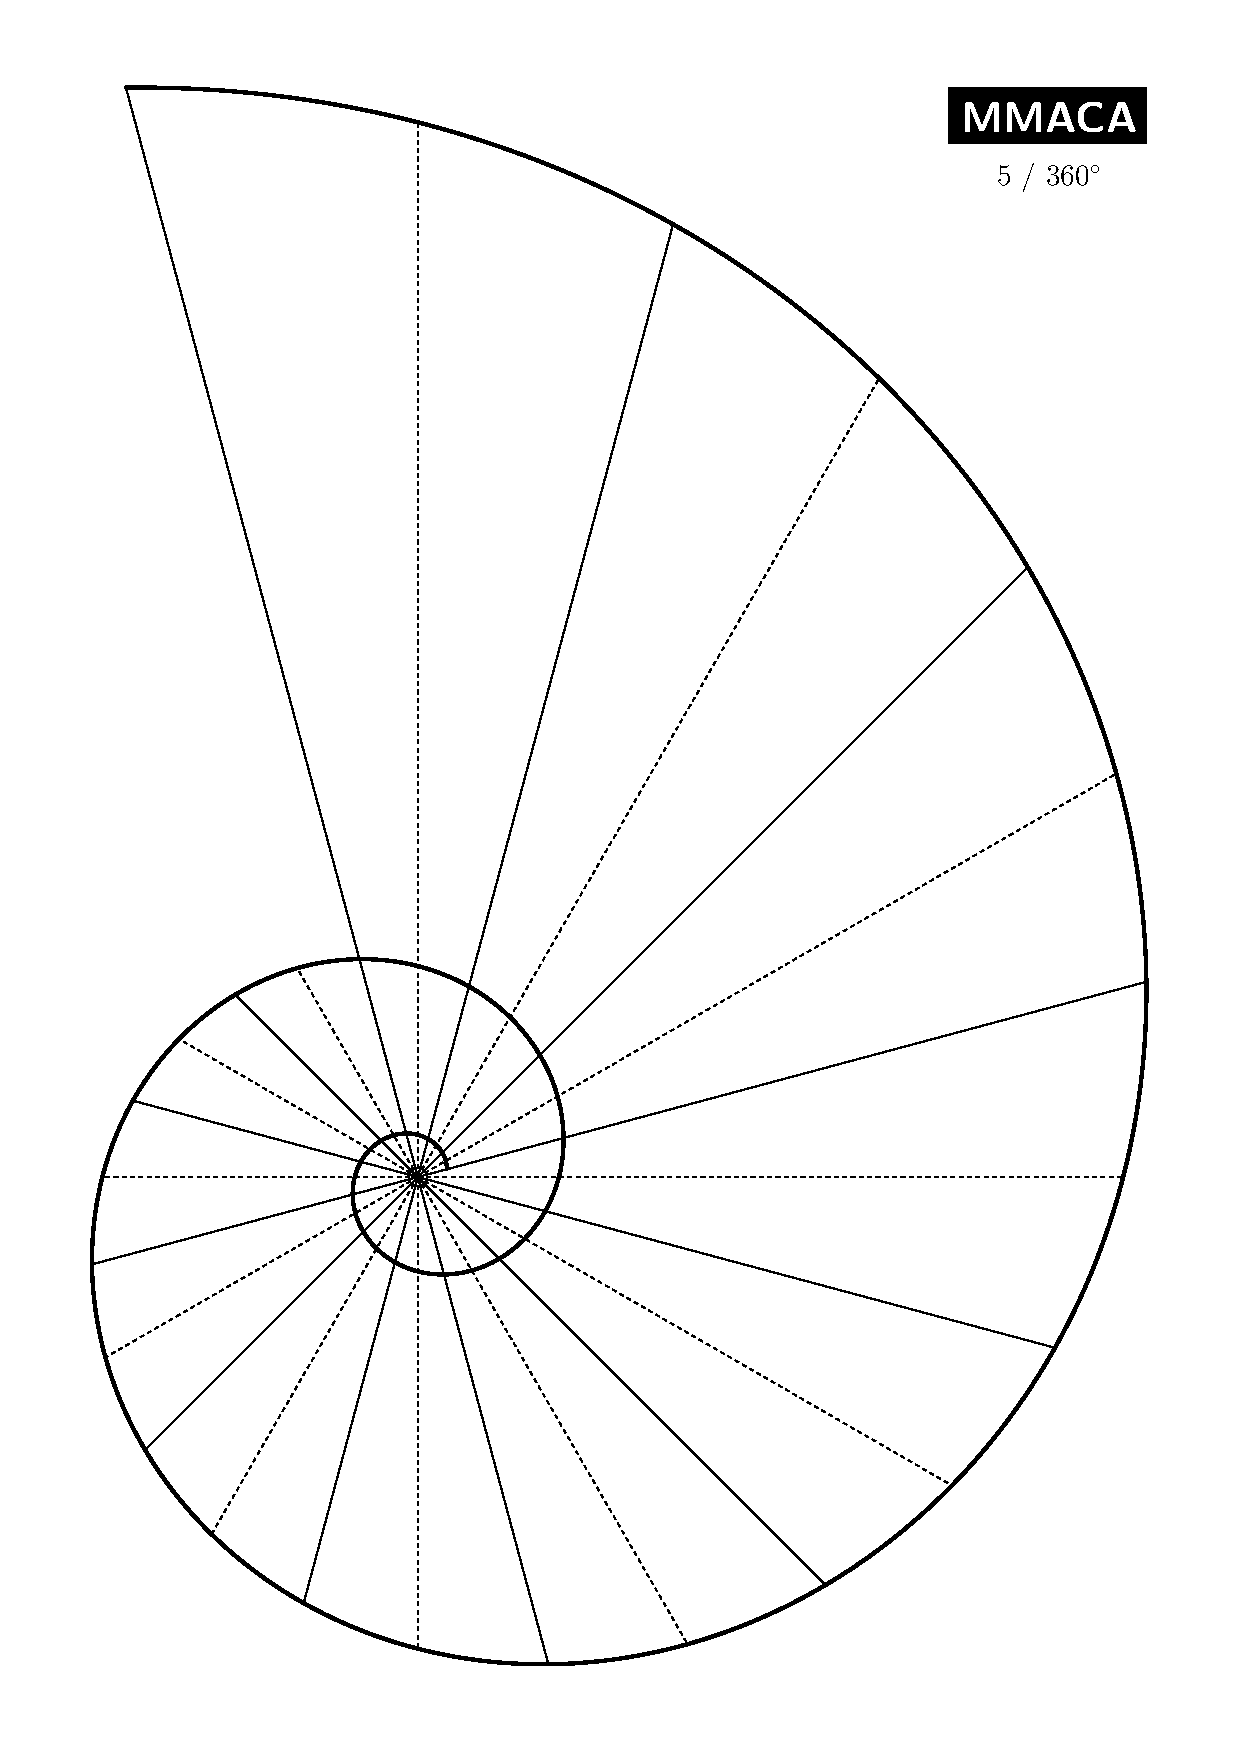
\includepdf{./pictures/Spiral_5_360}
    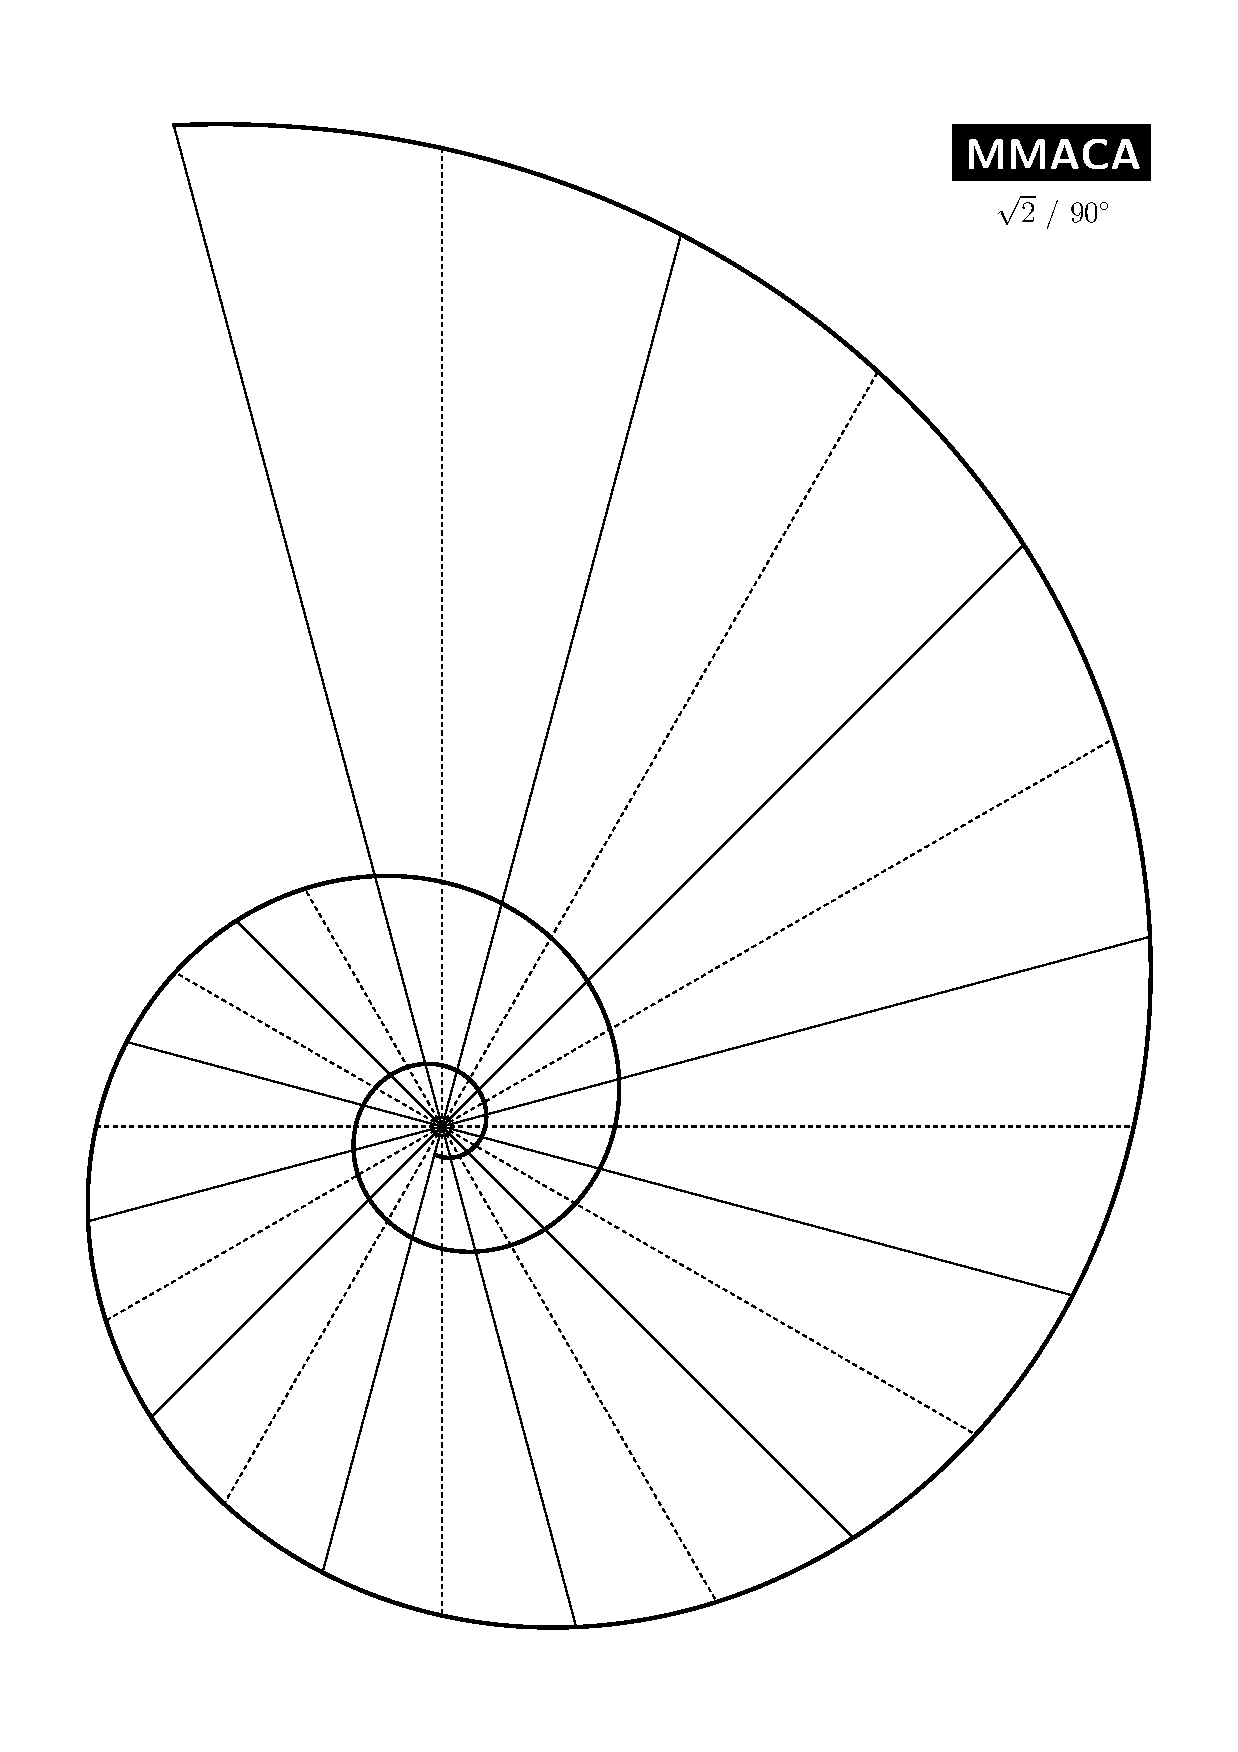
\includepdf{./pictures/Spiral_Root2_090}
    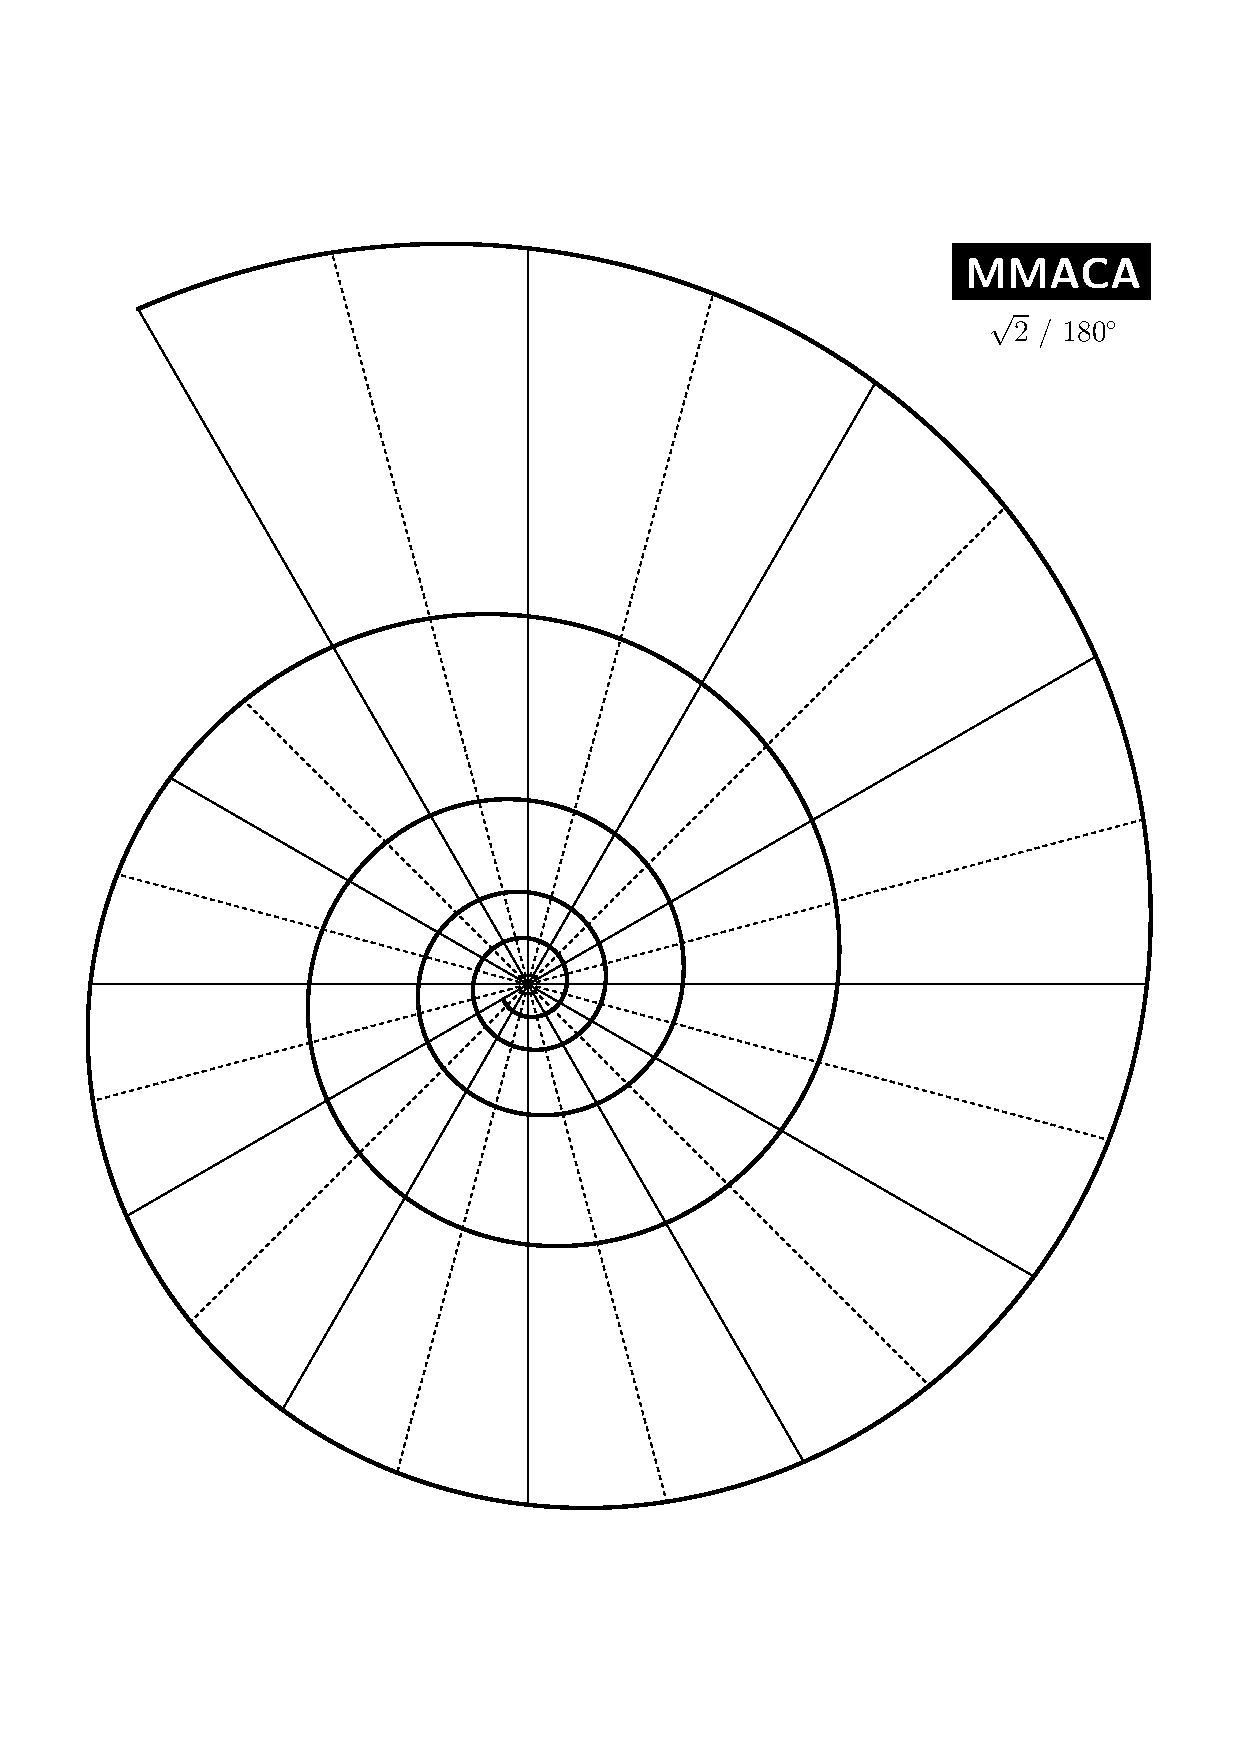
\includepdf{./pictures/Spiral_Root2_180}
    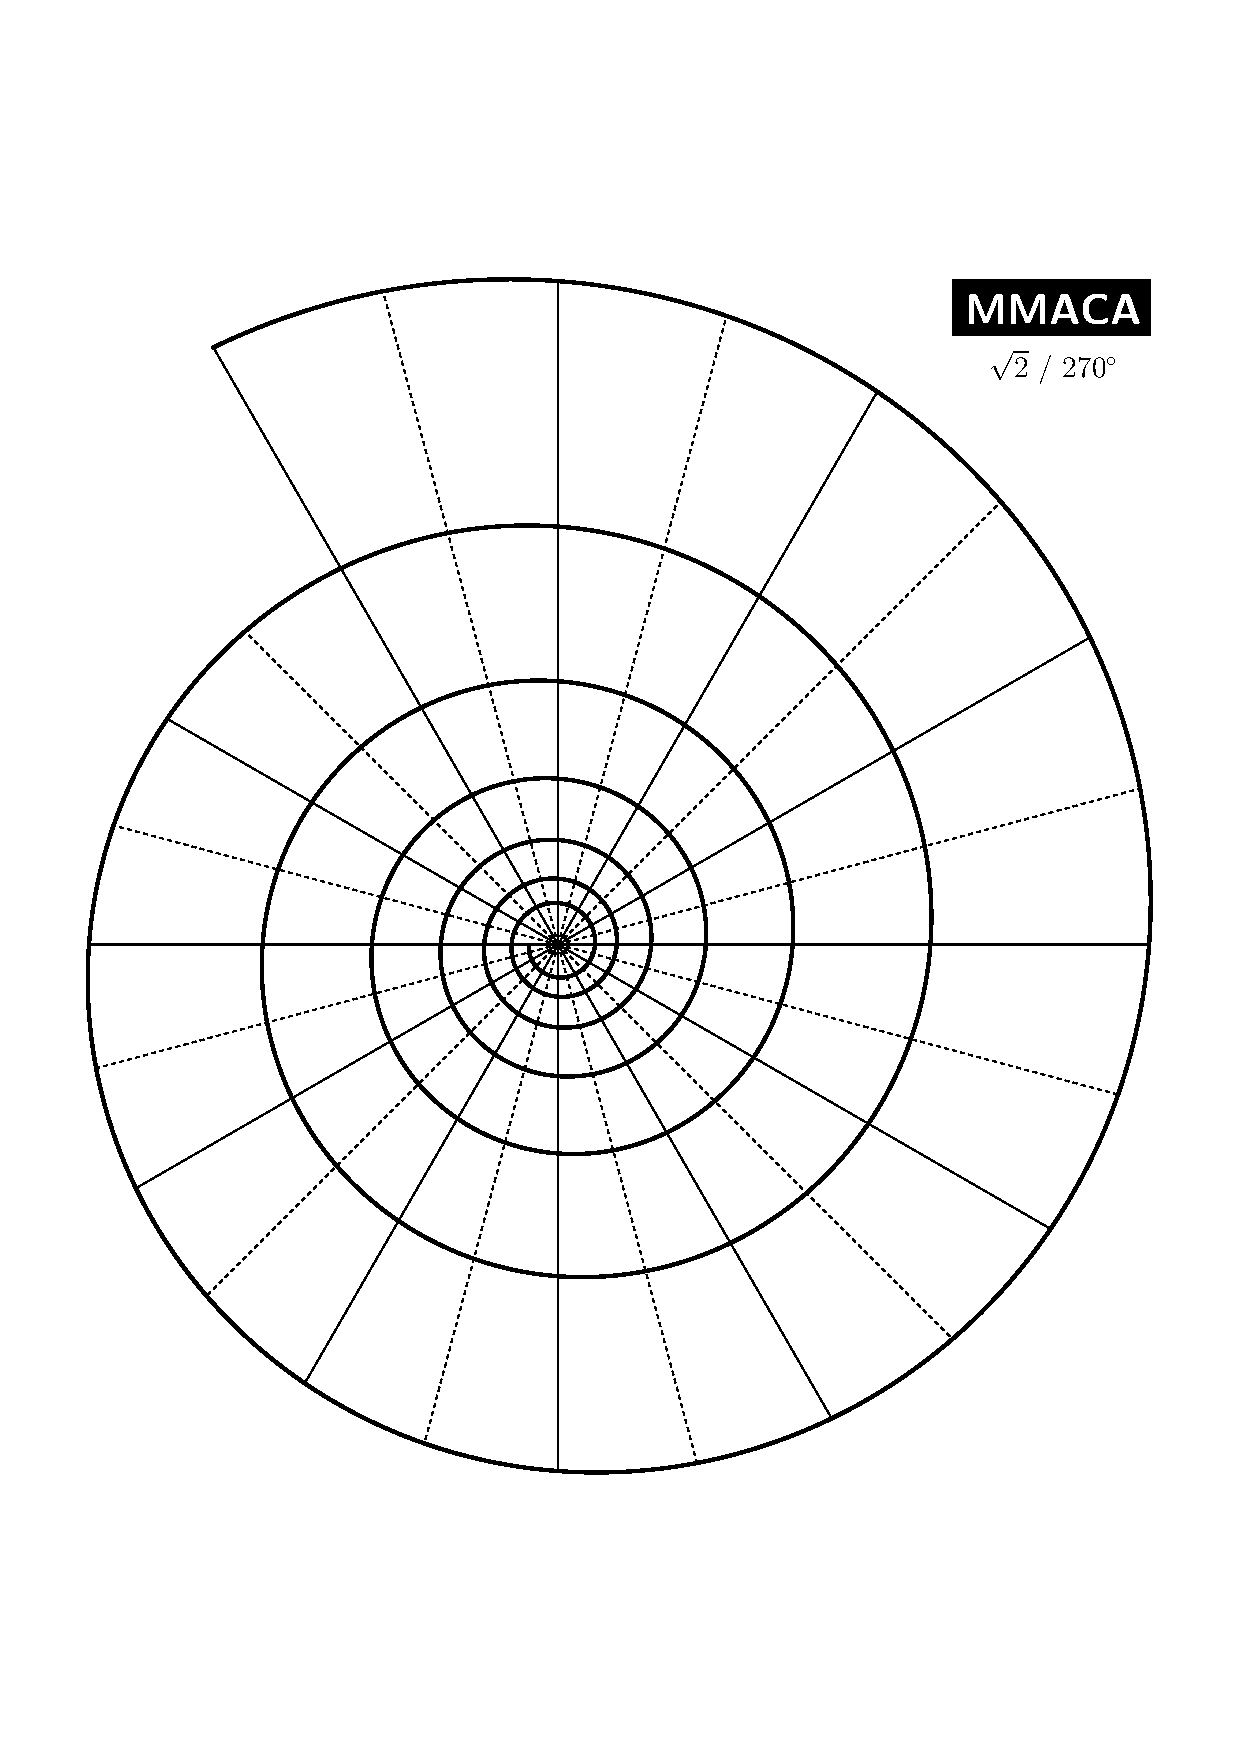
\includepdf{./pictures/Spiral_Root2_270}
    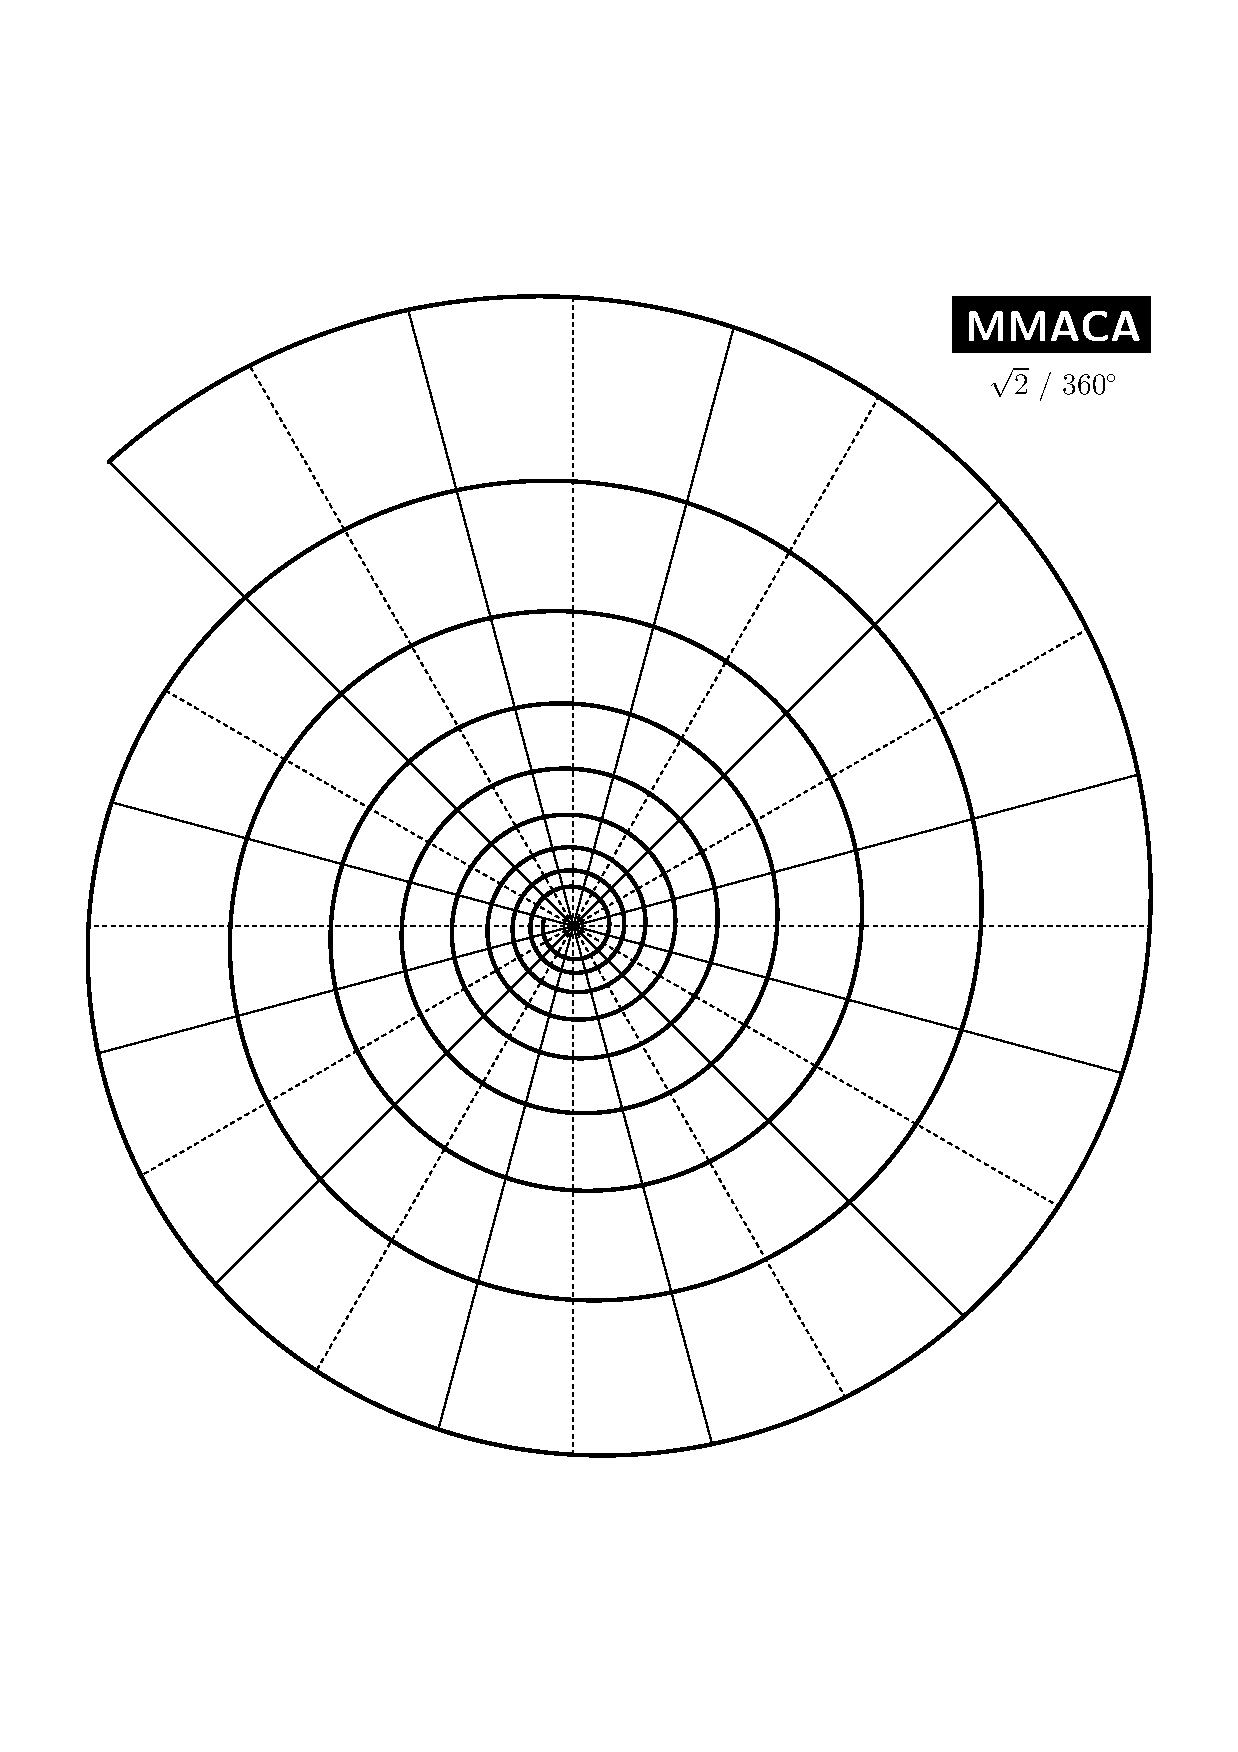
\includepdf{./pictures/Spiral_Root2_360}
    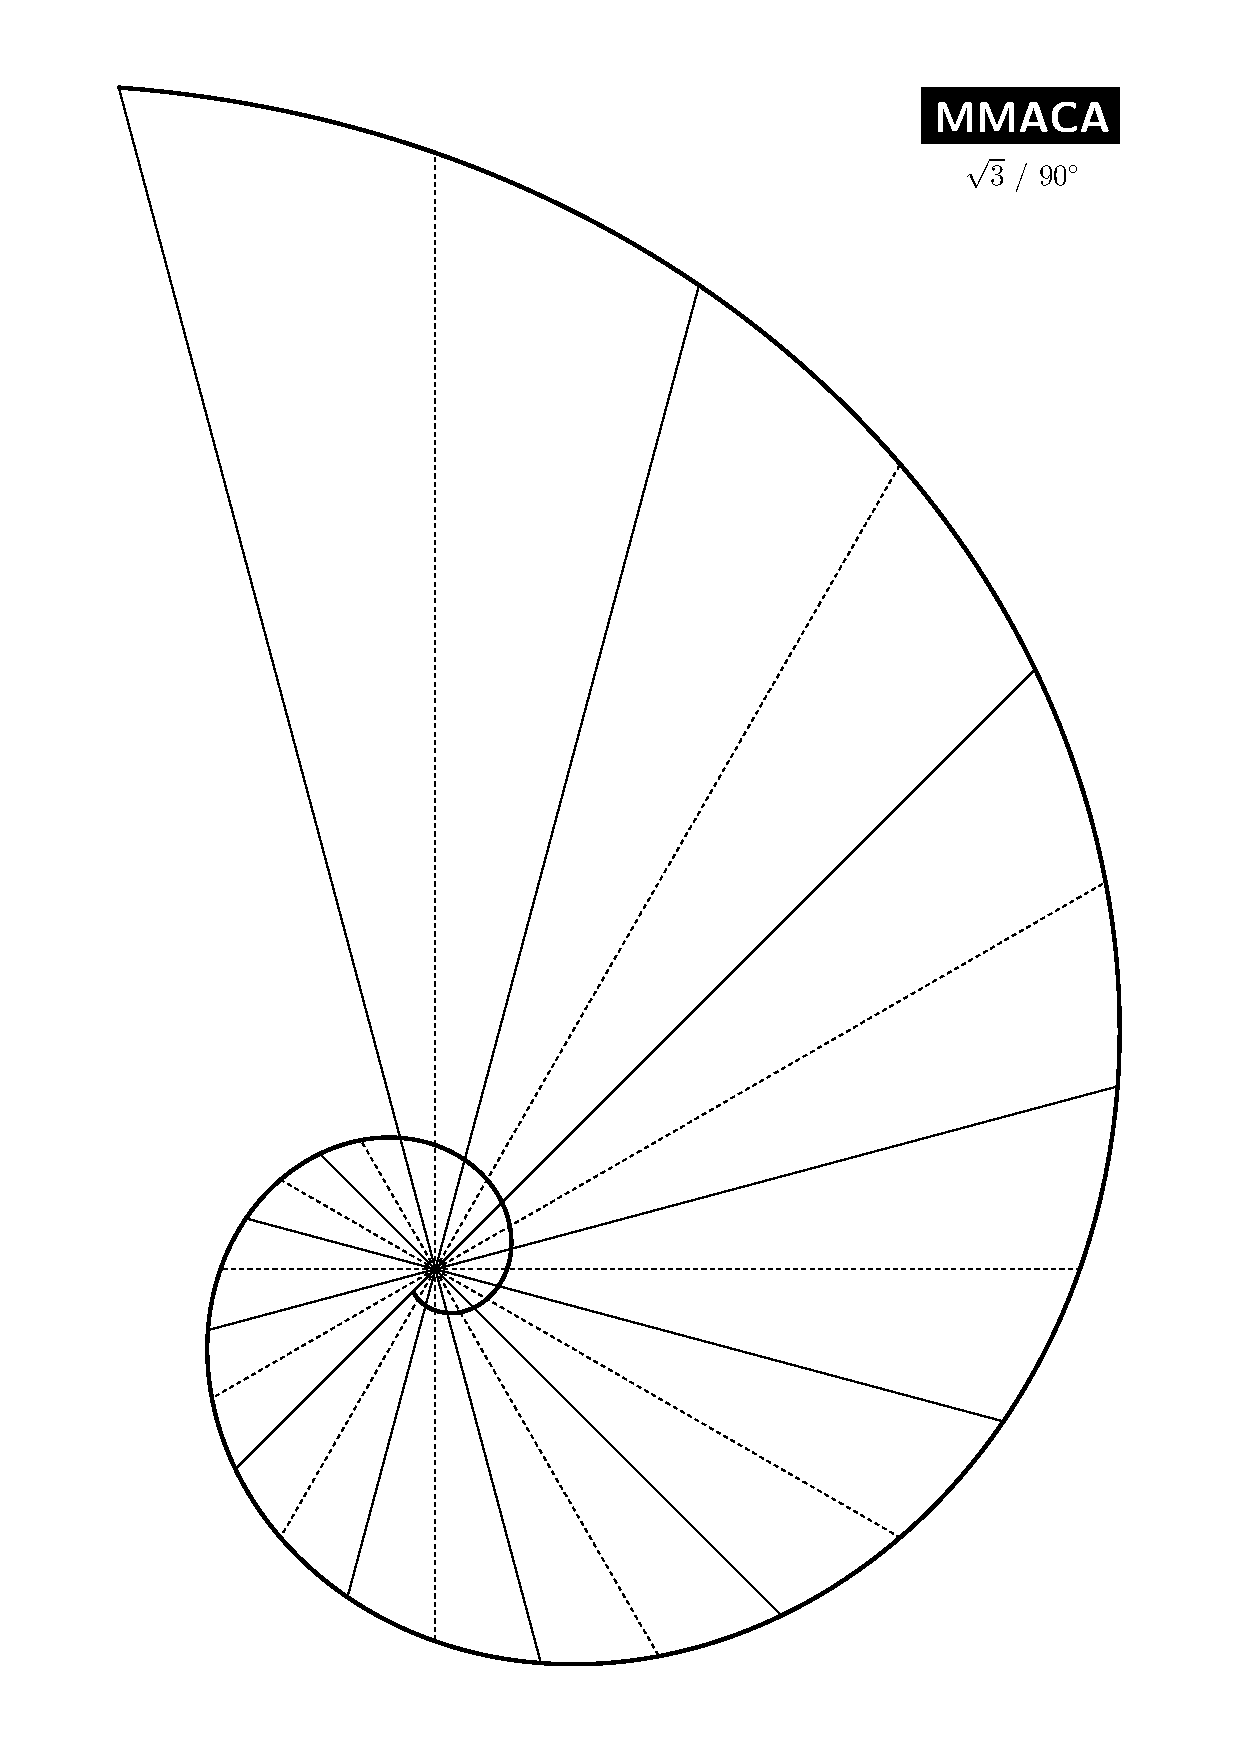
\includepdf{./pictures/Spiral_Root3_090}
    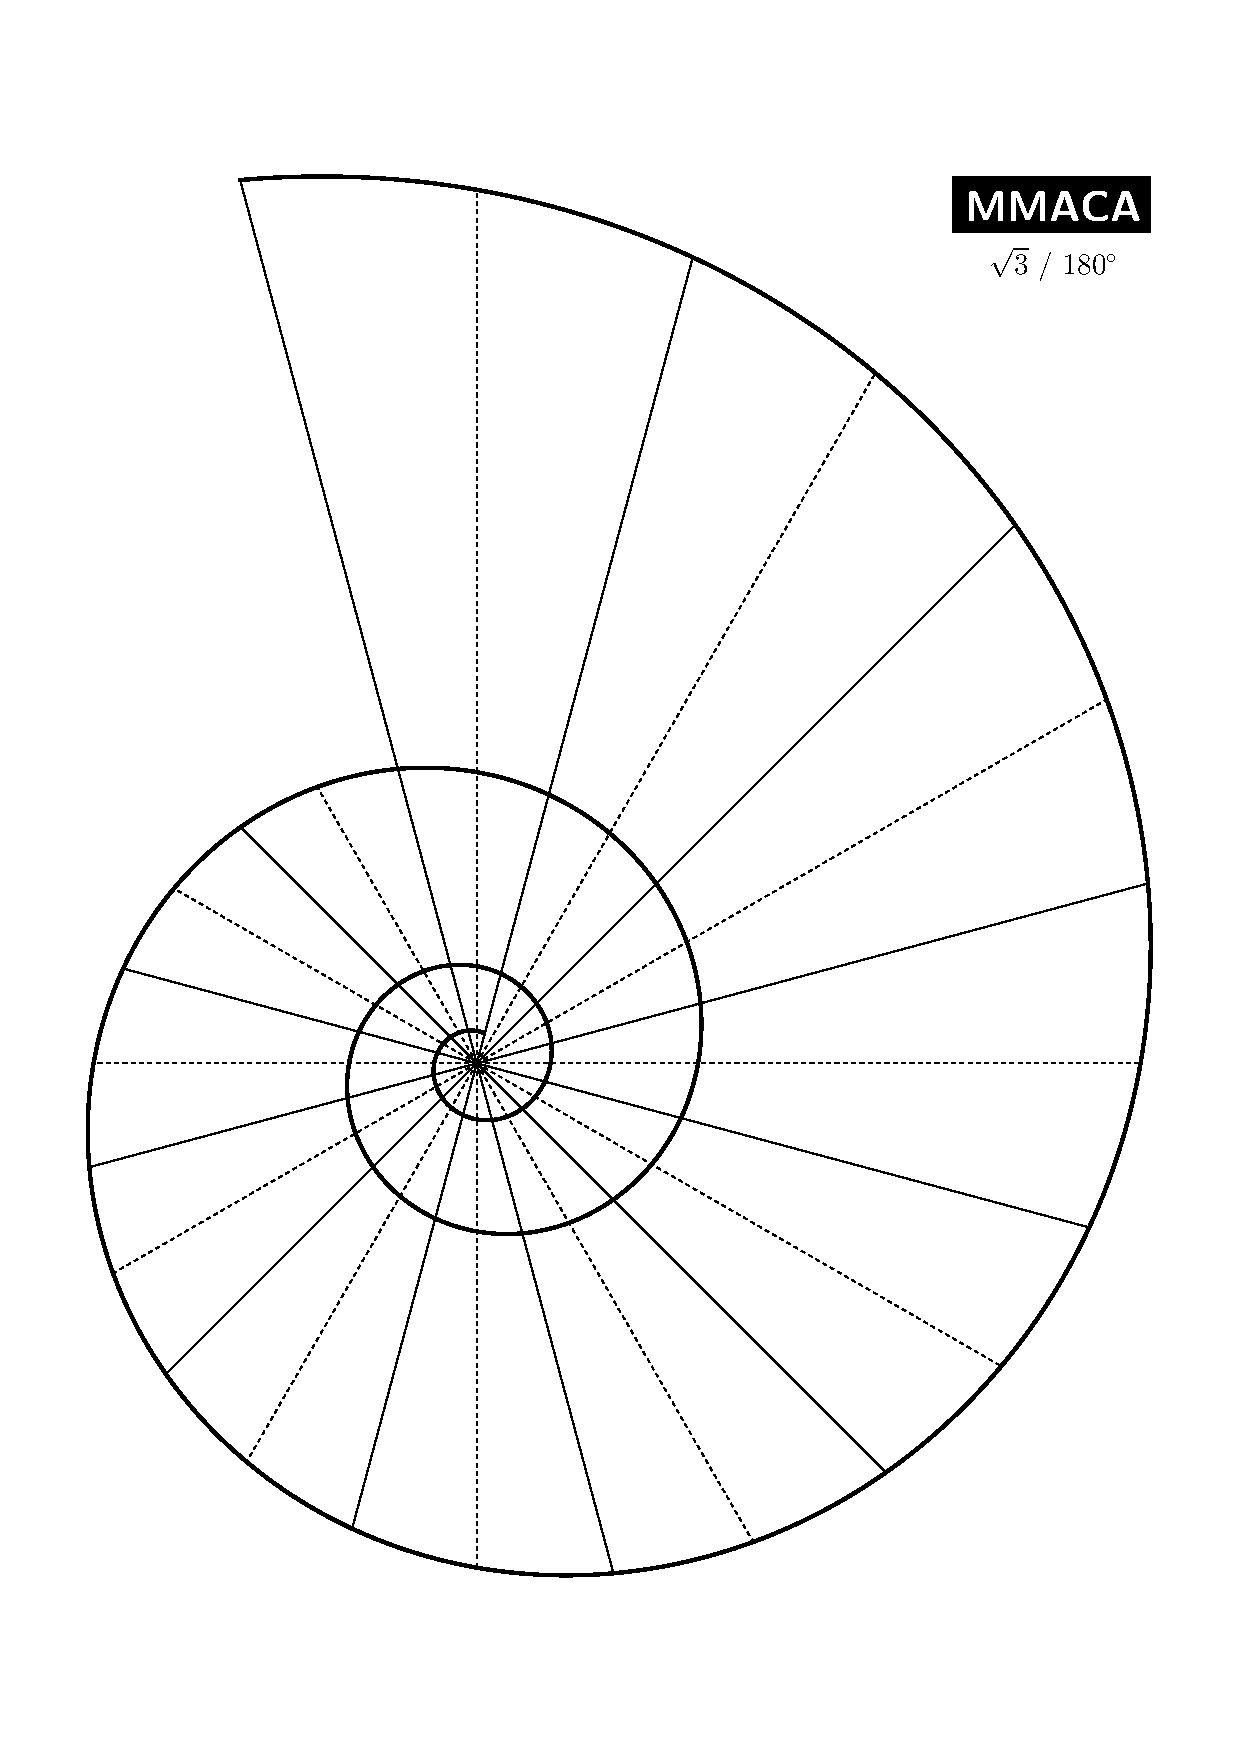
\includepdf{./pictures/Spiral_Root3_180}
    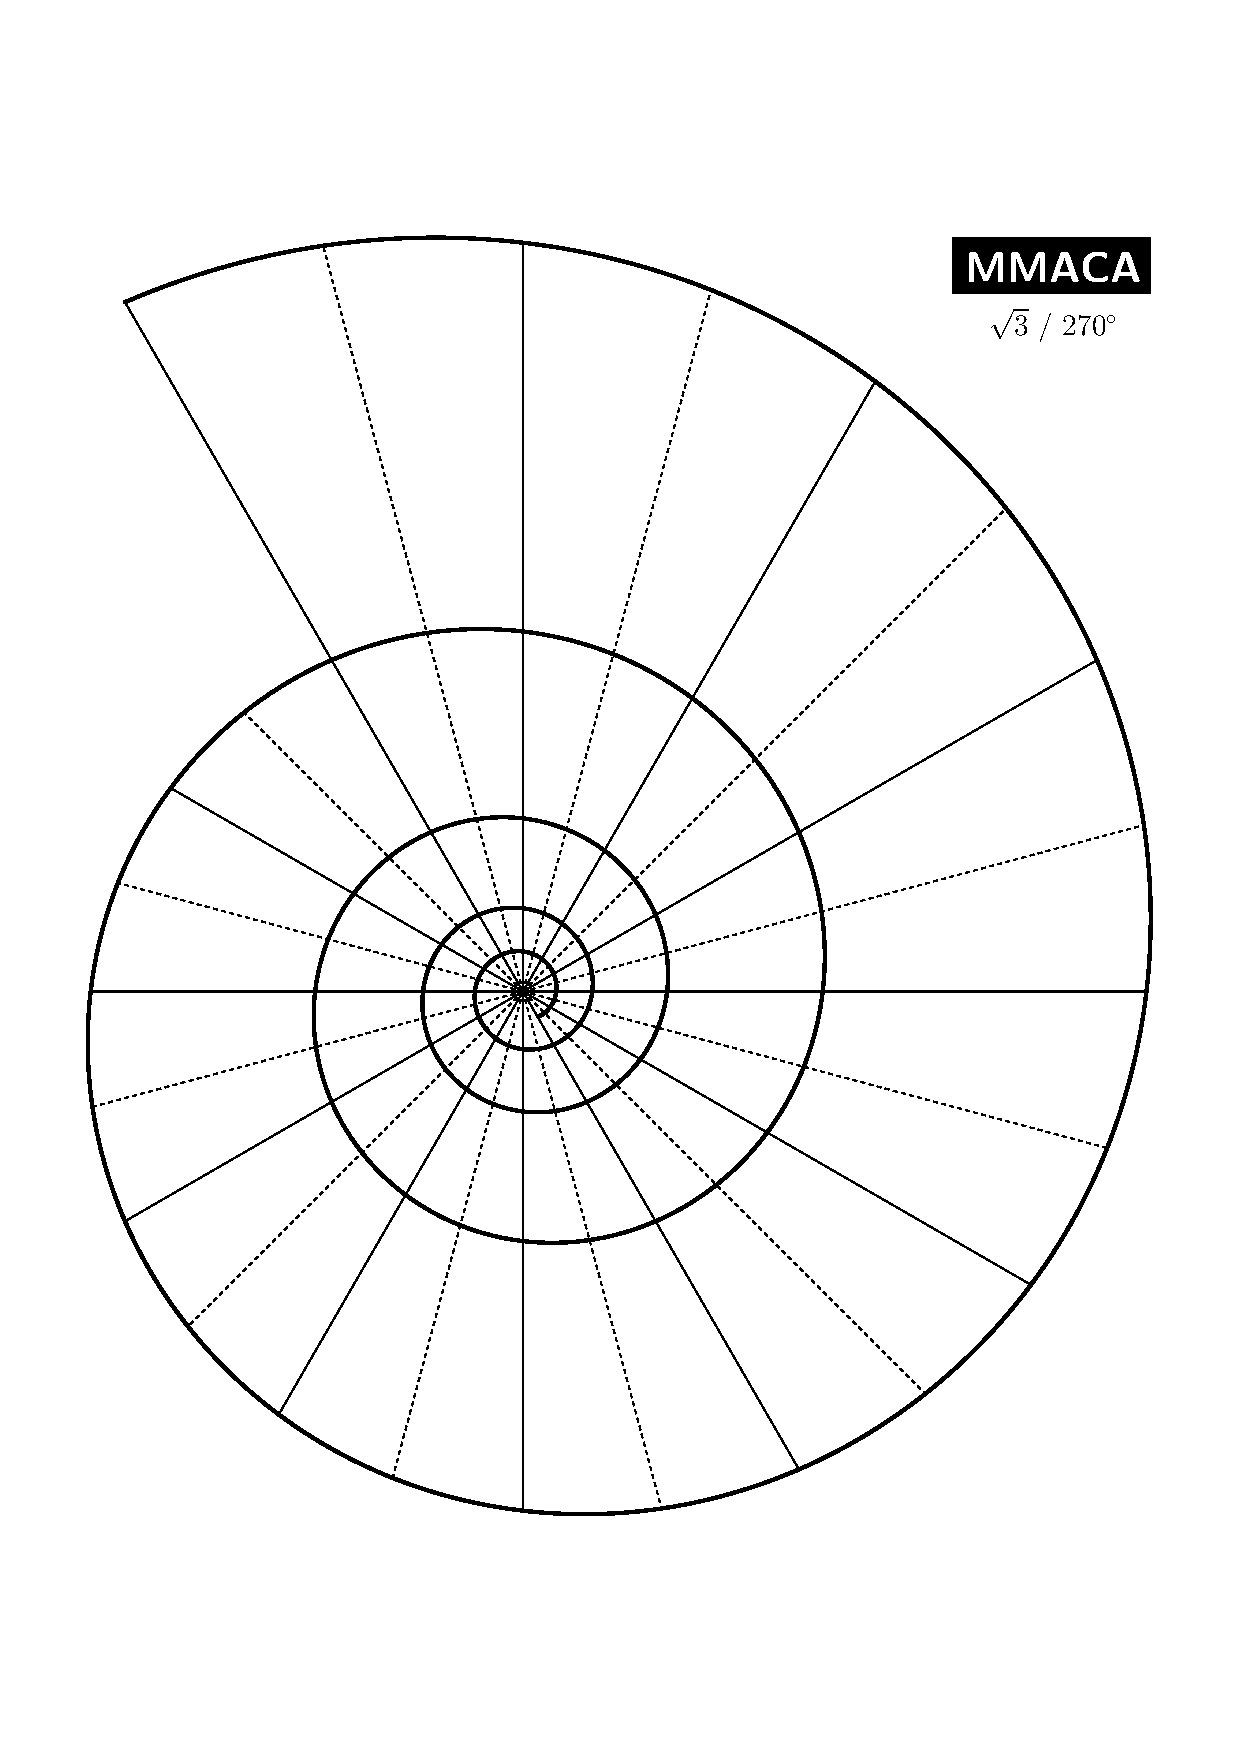
\includepdf{./pictures/Spiral_Root3_270}
    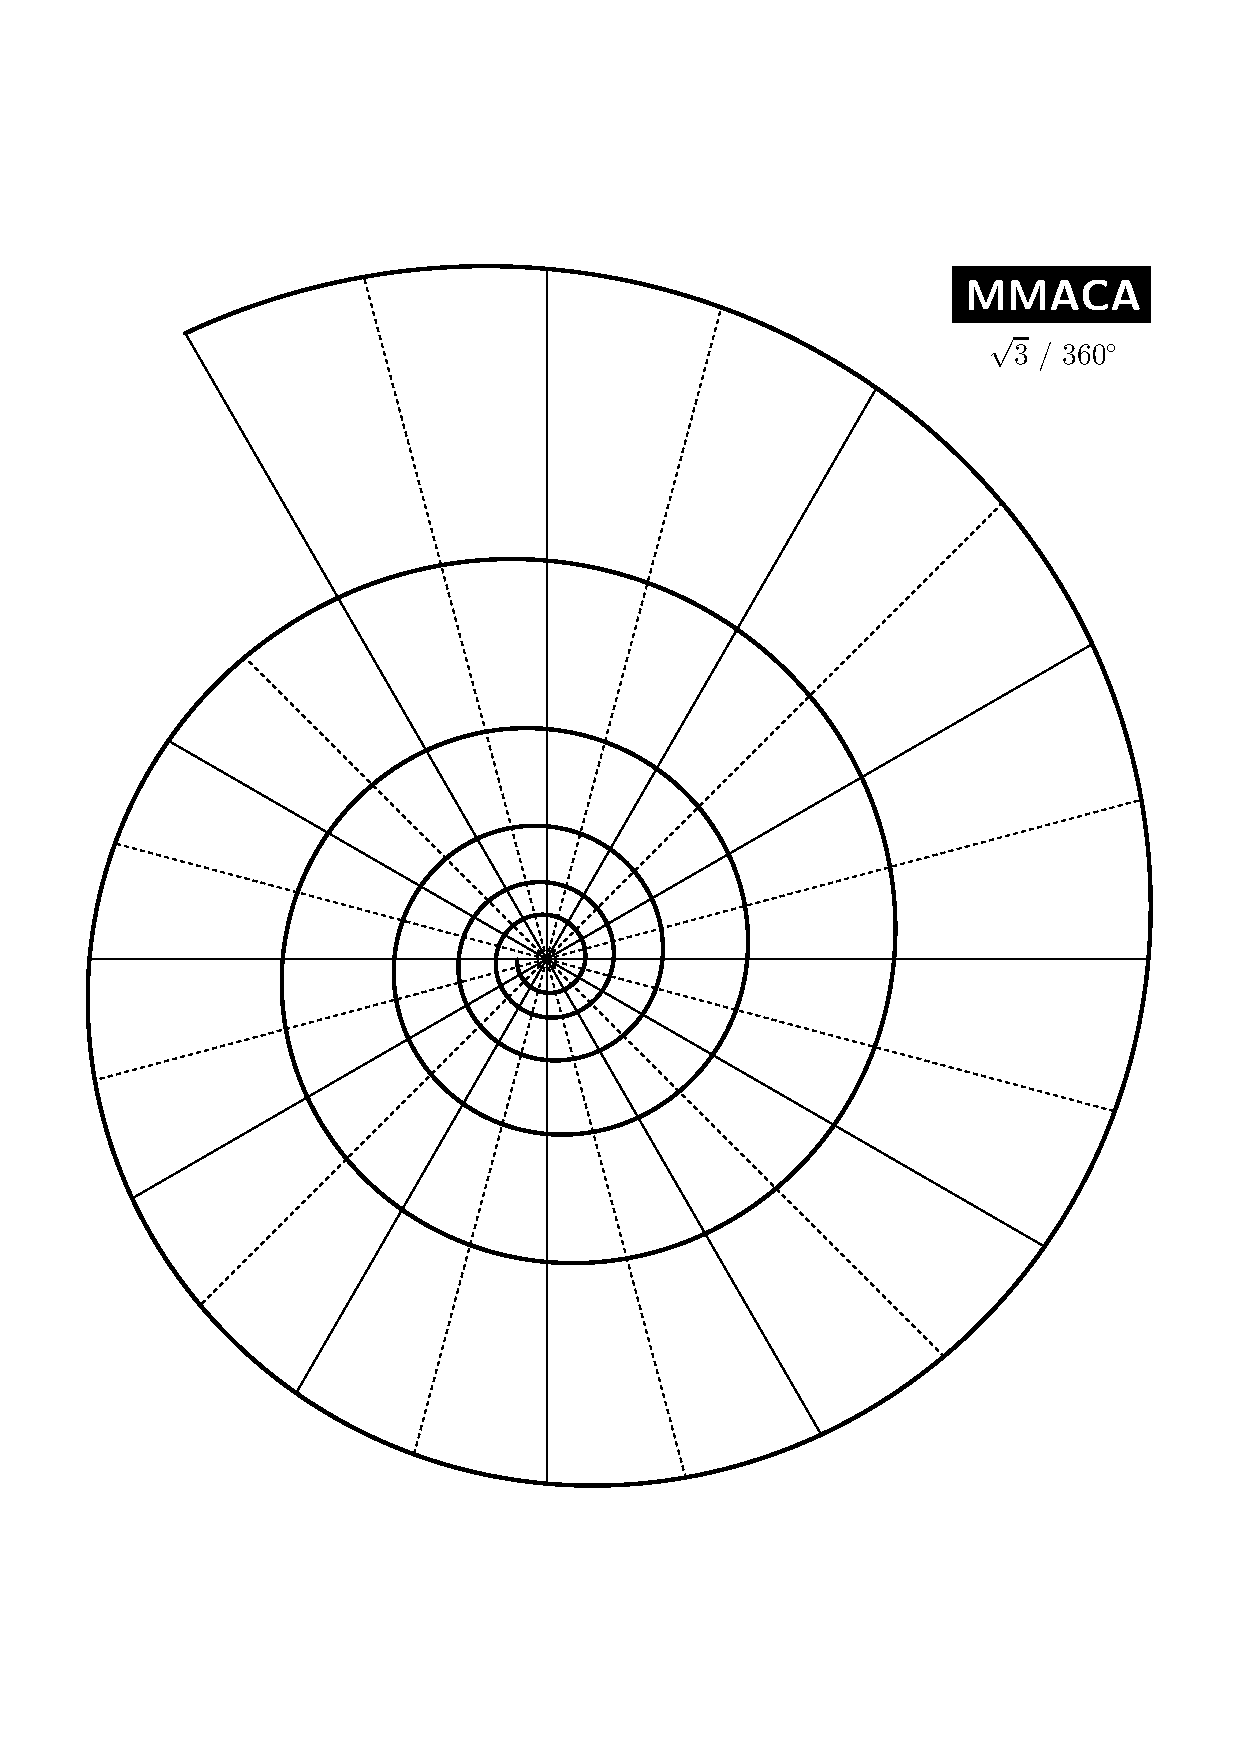
\includepdf{./pictures/Spiral_Root3_360}
    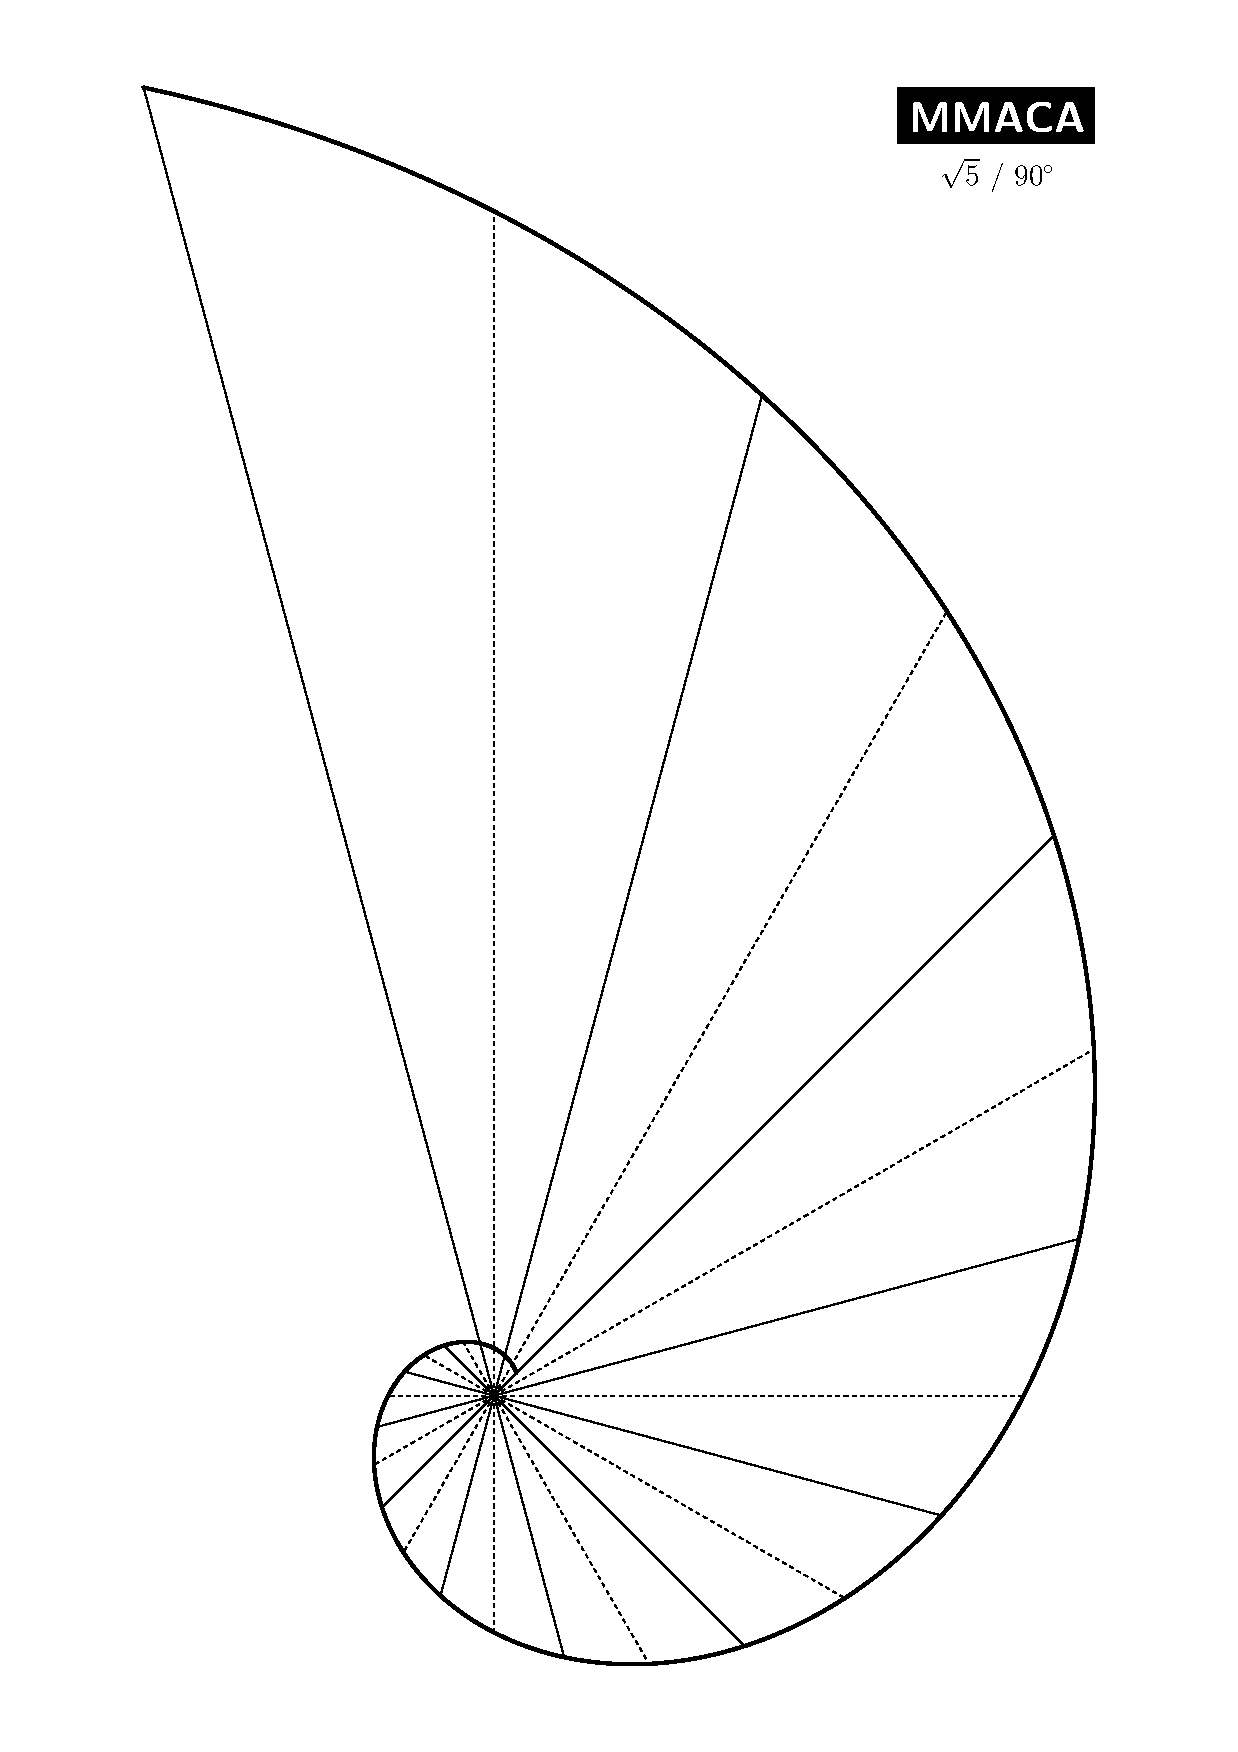
\includepdf{./pictures/Spiral_Root5_090}
    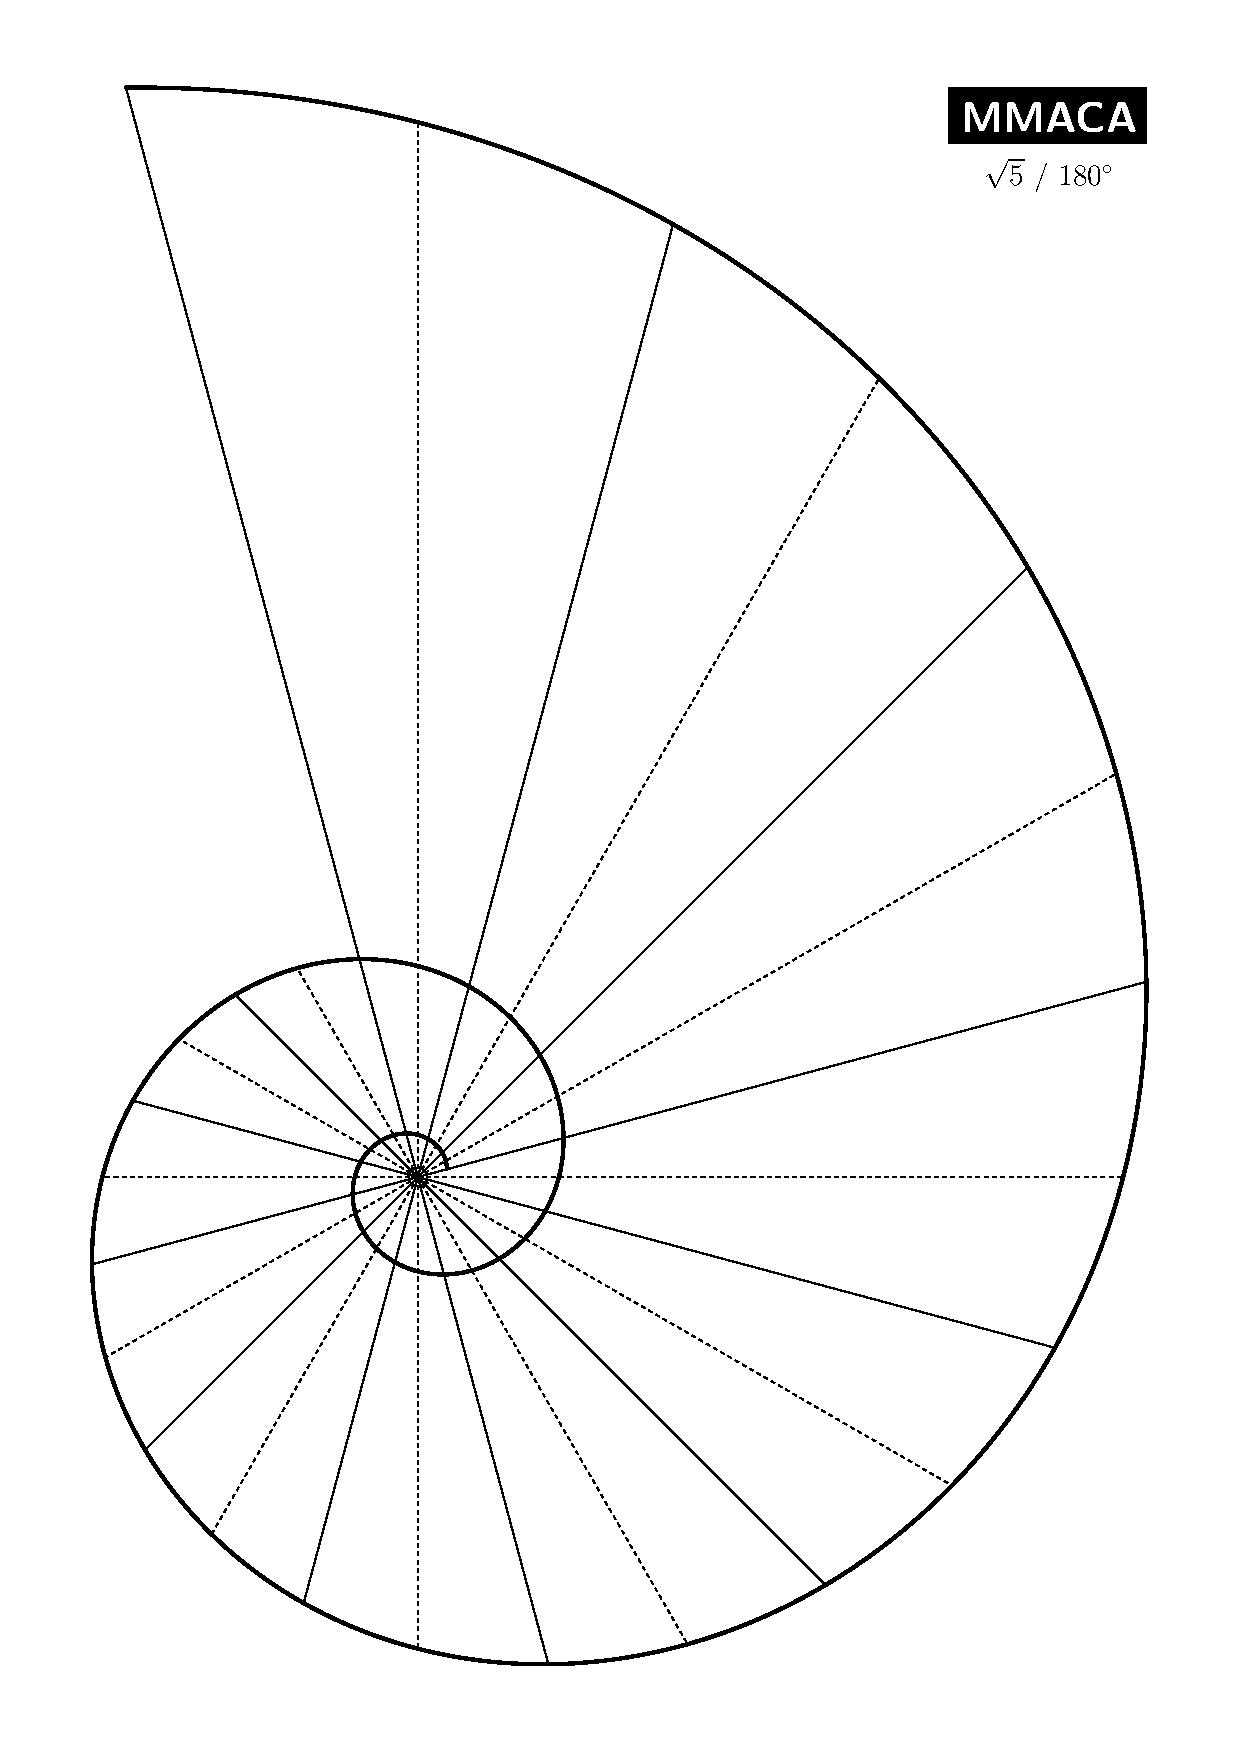
\includepdf{./pictures/Spiral_Root5_180}
    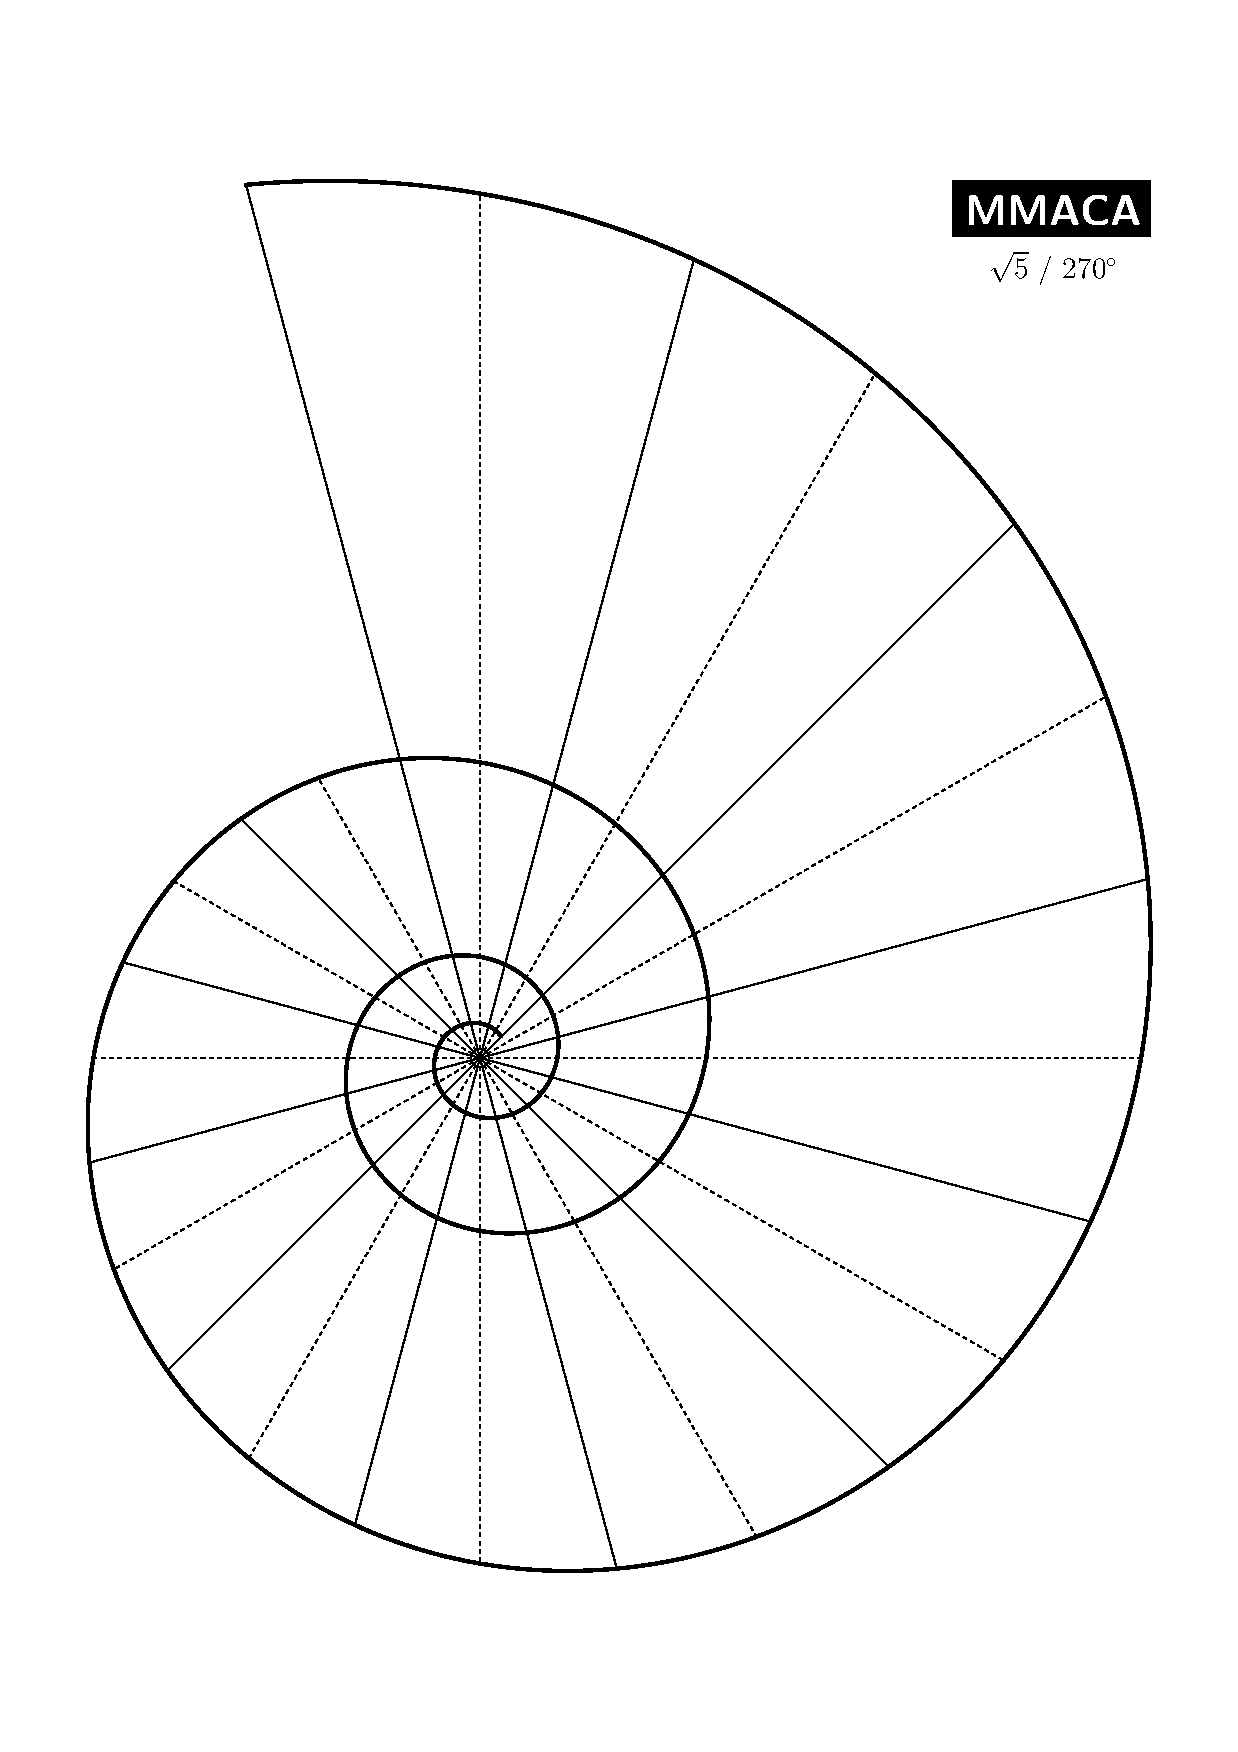
\includepdf{./pictures/Spiral_Root5_270}
    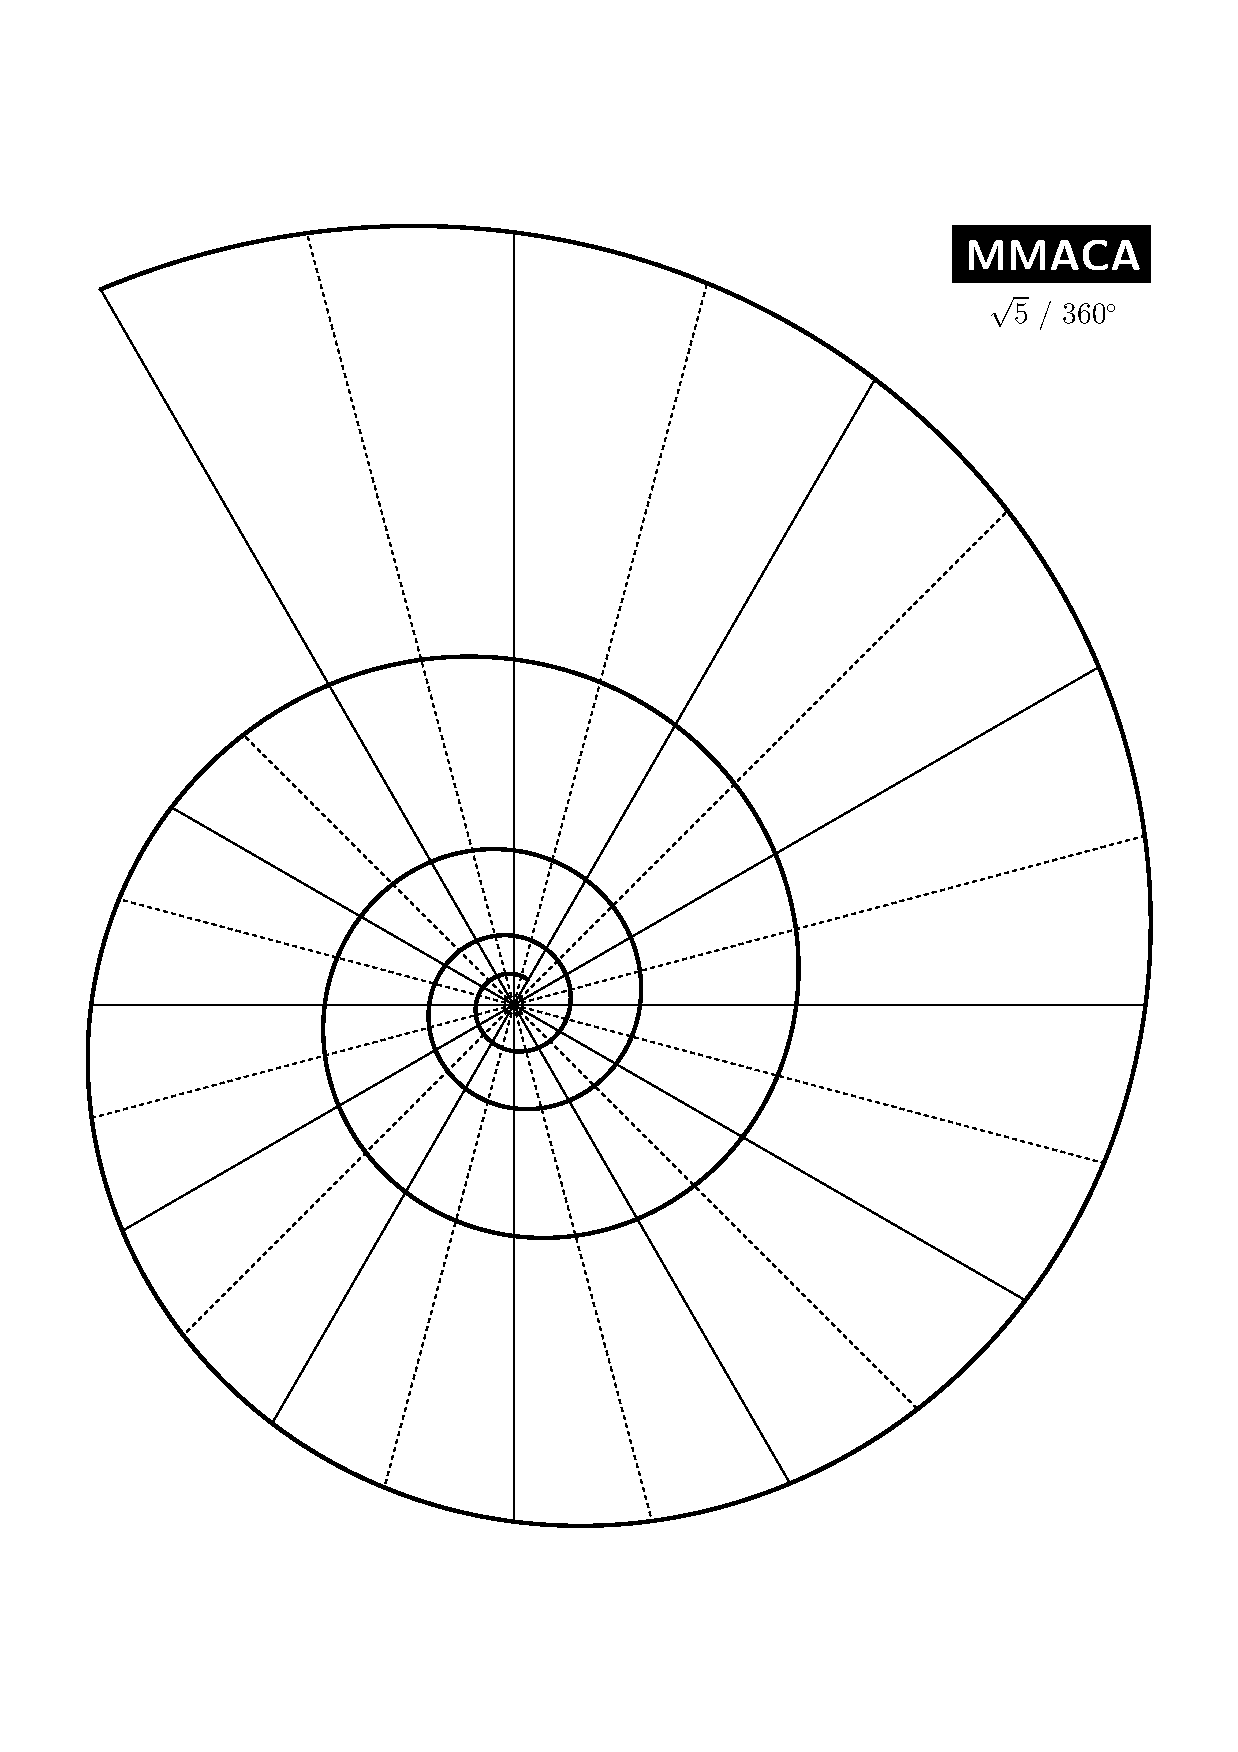
\includepdf{./pictures/Spiral_Root5_360}
    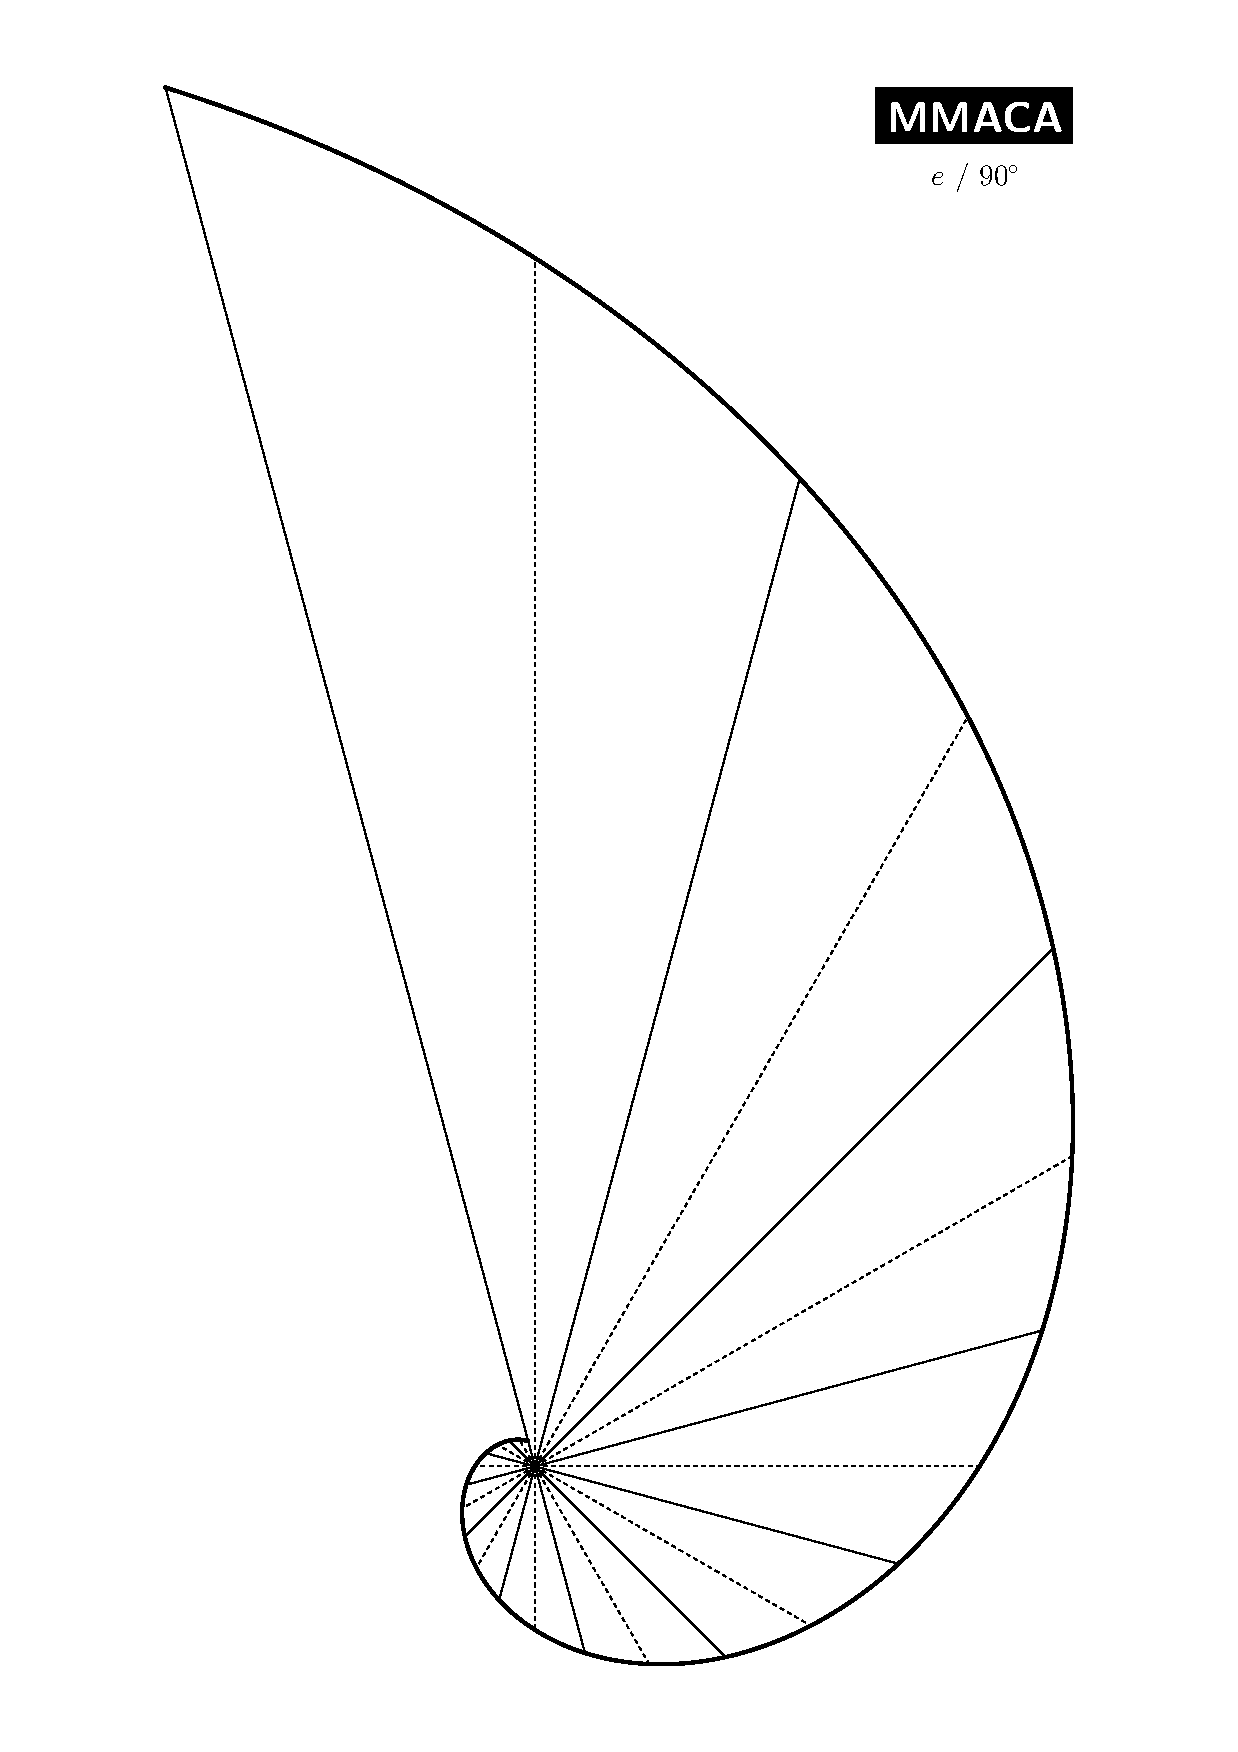
\includepdf{./pictures/Spiral_E_090}
    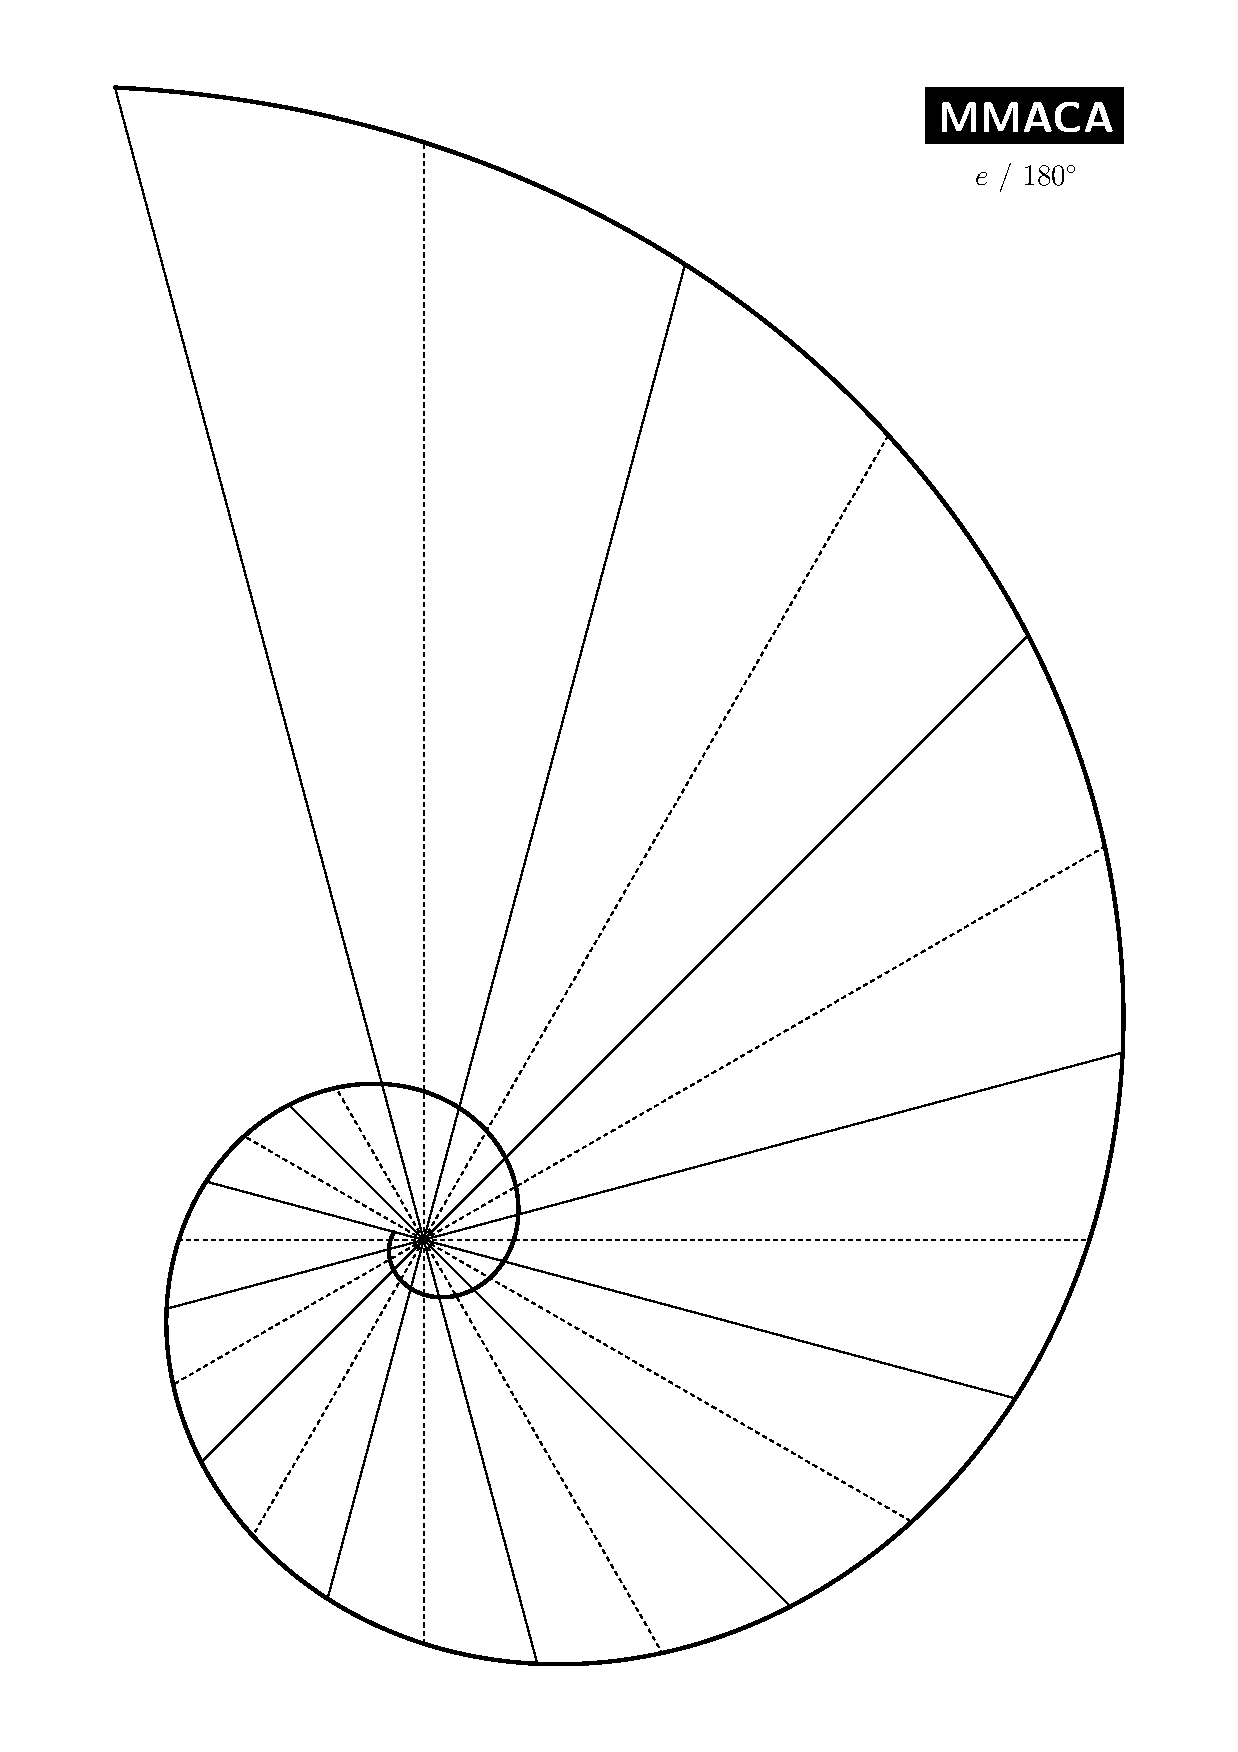
\includepdf{./pictures/Spiral_E_180}
    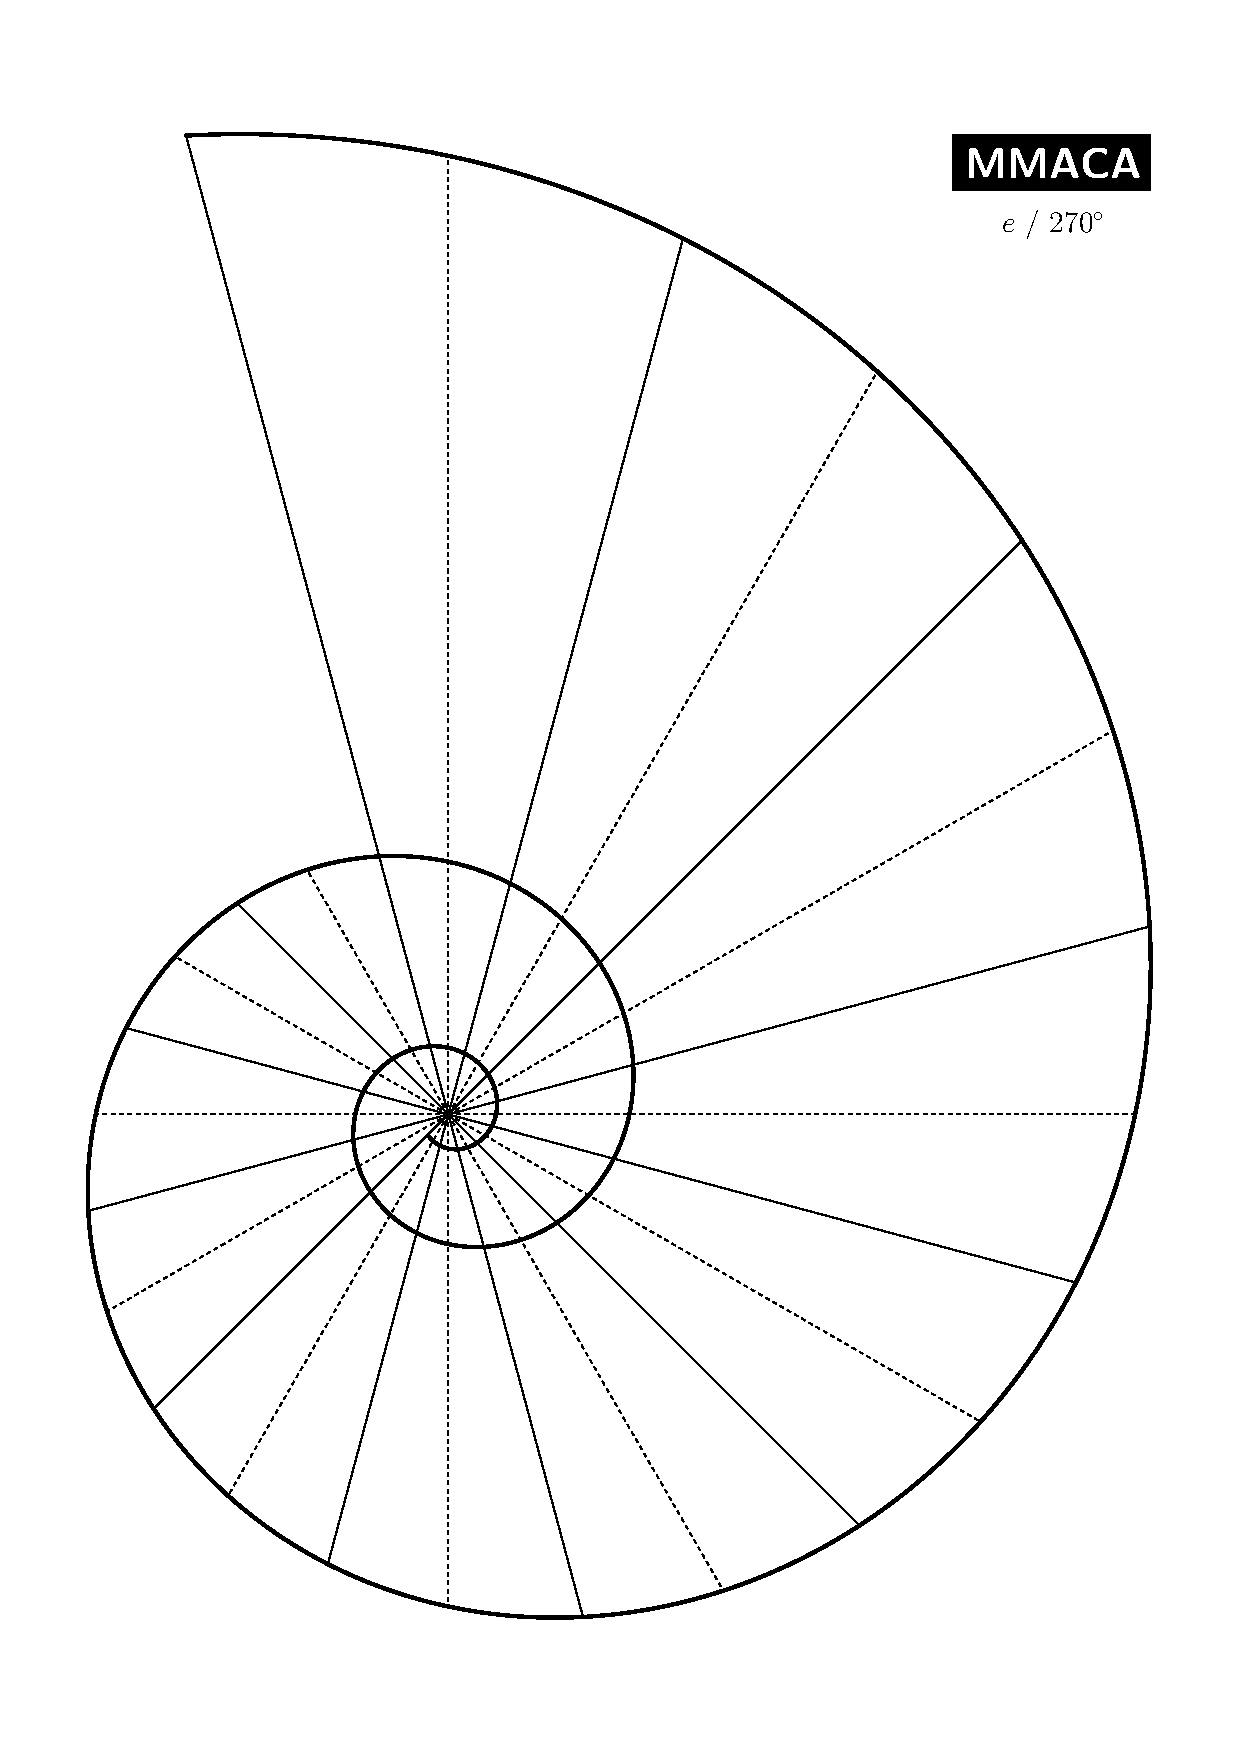
\includepdf{./pictures/Spiral_E_270}
    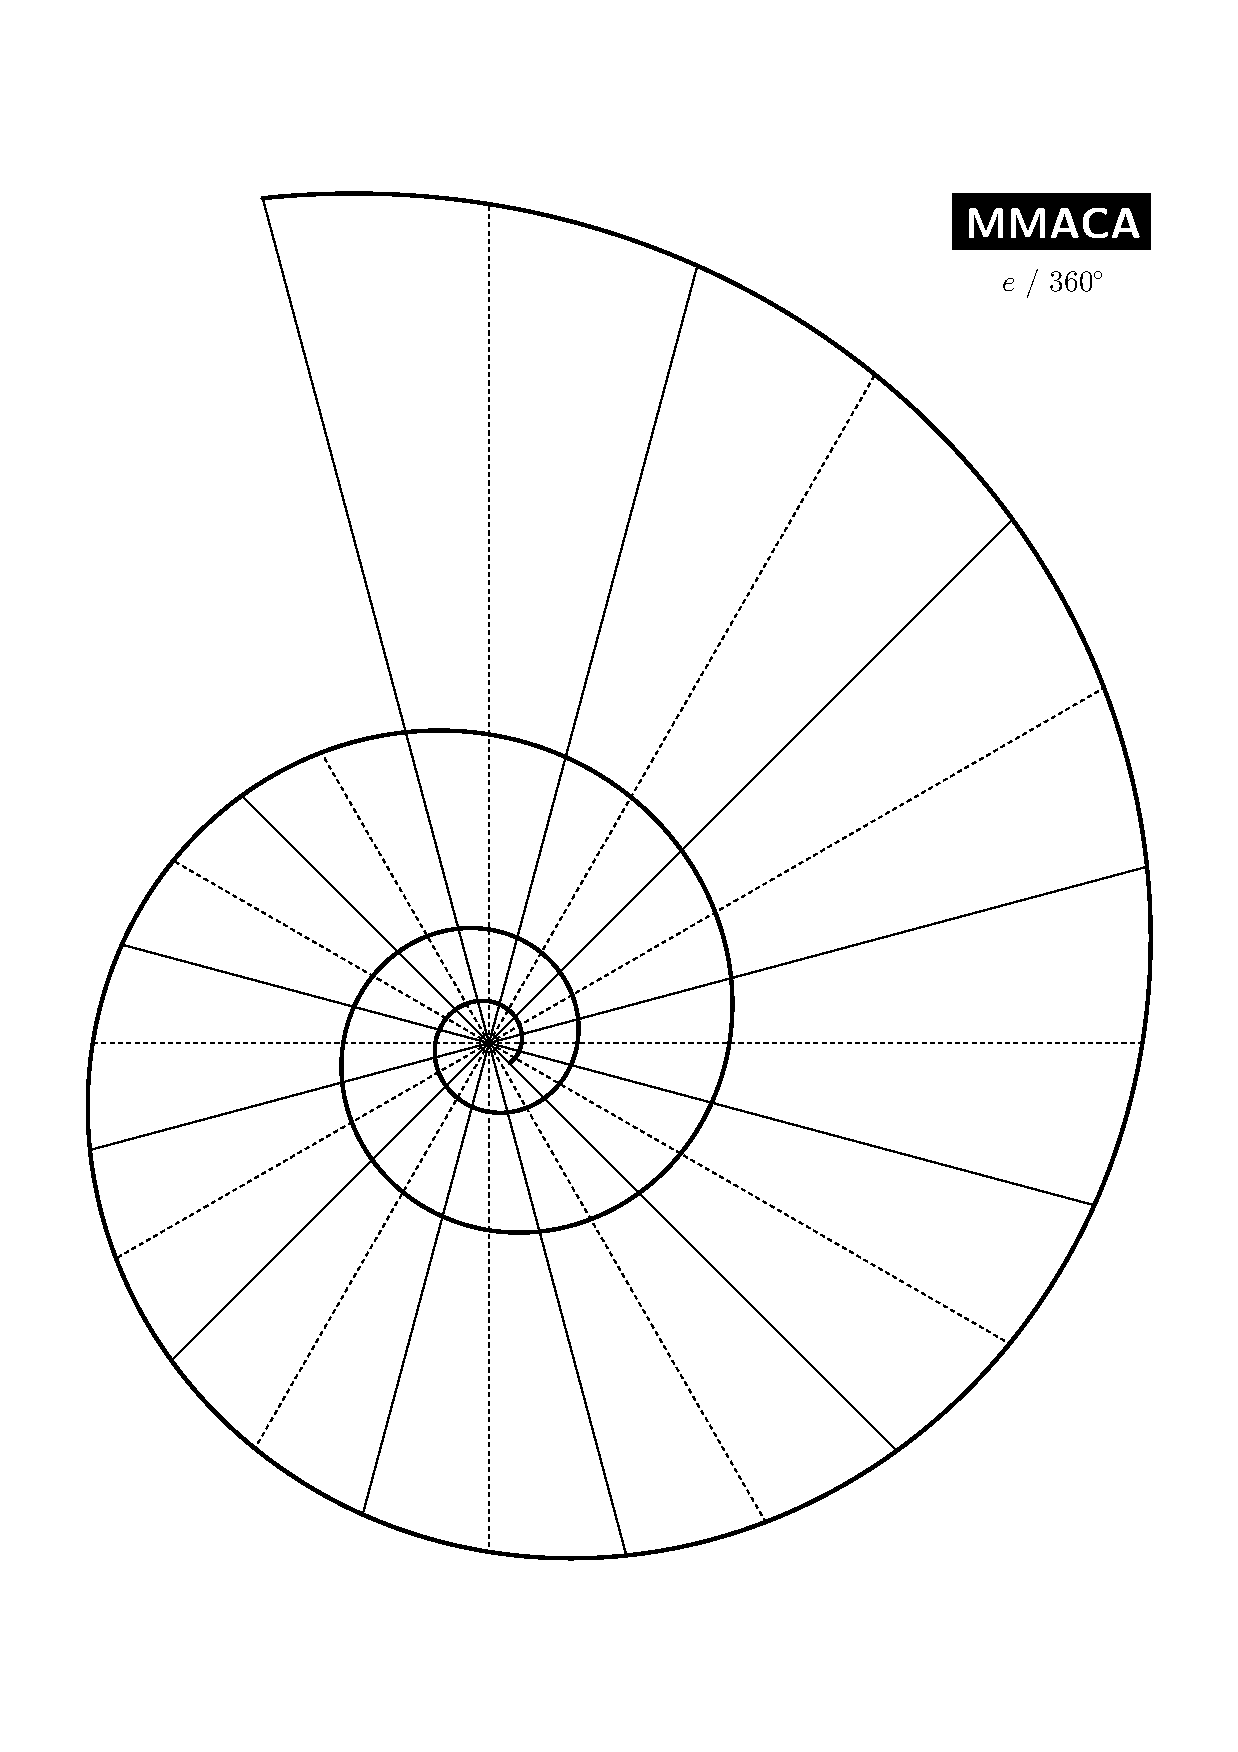
\includepdf{./pictures/Spiral_E_360}
    \includepdf{./pictures/Spiral_Pi_090}
    \includepdf{./pictures/Spiral_Pi_180}
    \includepdf{./pictures/Spiral_Pi_270}
    \includepdf{./pictures/Spiral_Pi_360}
    \includepdf{./pictures/Spiral_Phi_090}
    \includepdf{./pictures/Spiral_Phi_180}
    \includepdf{./pictures/Spiral_Phi_270}
    \includepdf{./pictures/Spiral_Phi_360}
    
    %%%%%%%%%%%%%%%%%%%%%%%%%%%%%%%%%%%%%%%%%%%%%%%%%%%%%%%%%%%%%%%%%%%%%%%%%%%%
    
\end{document}
